\section{Object definition and selection}
We have seen in~\ref{sec:reconstruction-and-identification} how objects are being reconstructed and identified in our detector. We have also studied the signal signature in~\ref{sec:signal-signature}. In this section we devise an object selection in order to obtain as pure as possible sample of objects in regards to our target leptons, while retaining as much signal as possible. As we have seen in ~\ref{sec:search-strategy}, we are targeting the opposite-charged same-flavor leptons \ellell that result from the \neutt that decays into a \neuto via a \PZstar, \ie, \neuttdecay. In the following section, we choose to present two choices of \gls{dmo}, namely, $\dmo=1.92\GeV$ and $\dmo=5.63\GeV$, \ie, a relatively high \gls{dmo}, and a low one, but not too low as to still be able to have enough electrons surviving the initial reconstruction \pt threshold of $5\GeV$. We also fix the higgsino parameter on $\mu=100\GeV$.

As was the case in~\ref{sec:signal-signature}, the base selection for the following section is requiring at least one jet in the event with $\pt \geq 30\GeV$ and $\abs{\eta}<2.4$. No other selections otherwise. However, unlike~\ref{sec:signal-signature}, we do not weight our objects to any luminosity, as we are interested in the proportion between object types. We differentiate between two types of leptons, ones that originate from our targeted decay \neuttdecay, which will be shown in blue, and those that do not, which we refer to as \emph{other}, and are shown in yellow. Leptons that are marked as resulting from the \neuttdecay decay, which we will refer to as \emph{signal leptons}, are done so by matching a reconstructed lepton to a generator level lepton, which has been checked to have the \neutt as its parent. Lepton marked as \emph{other}, either has been misreconstructed, misidentified or is a result of hadronisation process in a jet (such as the \gls{isr} jet). Our goal here is to select as many blue leptons as possible, while rejecting as many yellow ones as possible. In the following sections, we will refer to \emph{efficiency} as the proportion between the signal leptons passing a selection, divided by the initial number of signal leptons, and to \emph{purity} as the proportion between signal leptons (blue) and the sum of the signal leptons and \emph{other} leptons (yellow). So to rephrase our goal, we are interested in a selection that results in high-efficiency and high-purity. These two quantities can sometimes compete with each other and we have to make compromises.

\subsection{Electrons}

\subsubsection{Signal electron selection}

The electrons have an initial reconstruction \pt threshold of $5\GeV$. The initial working point choice for reconstructed electron is loose (see~\ref{sec:reconstruction-and-identification}). The first distribution we look at in regards to the electrons is their spatial separation from the leading jet in the event, $\DR(\jmath_1,\Pe)$.

\begin{figure}[h]
\centering
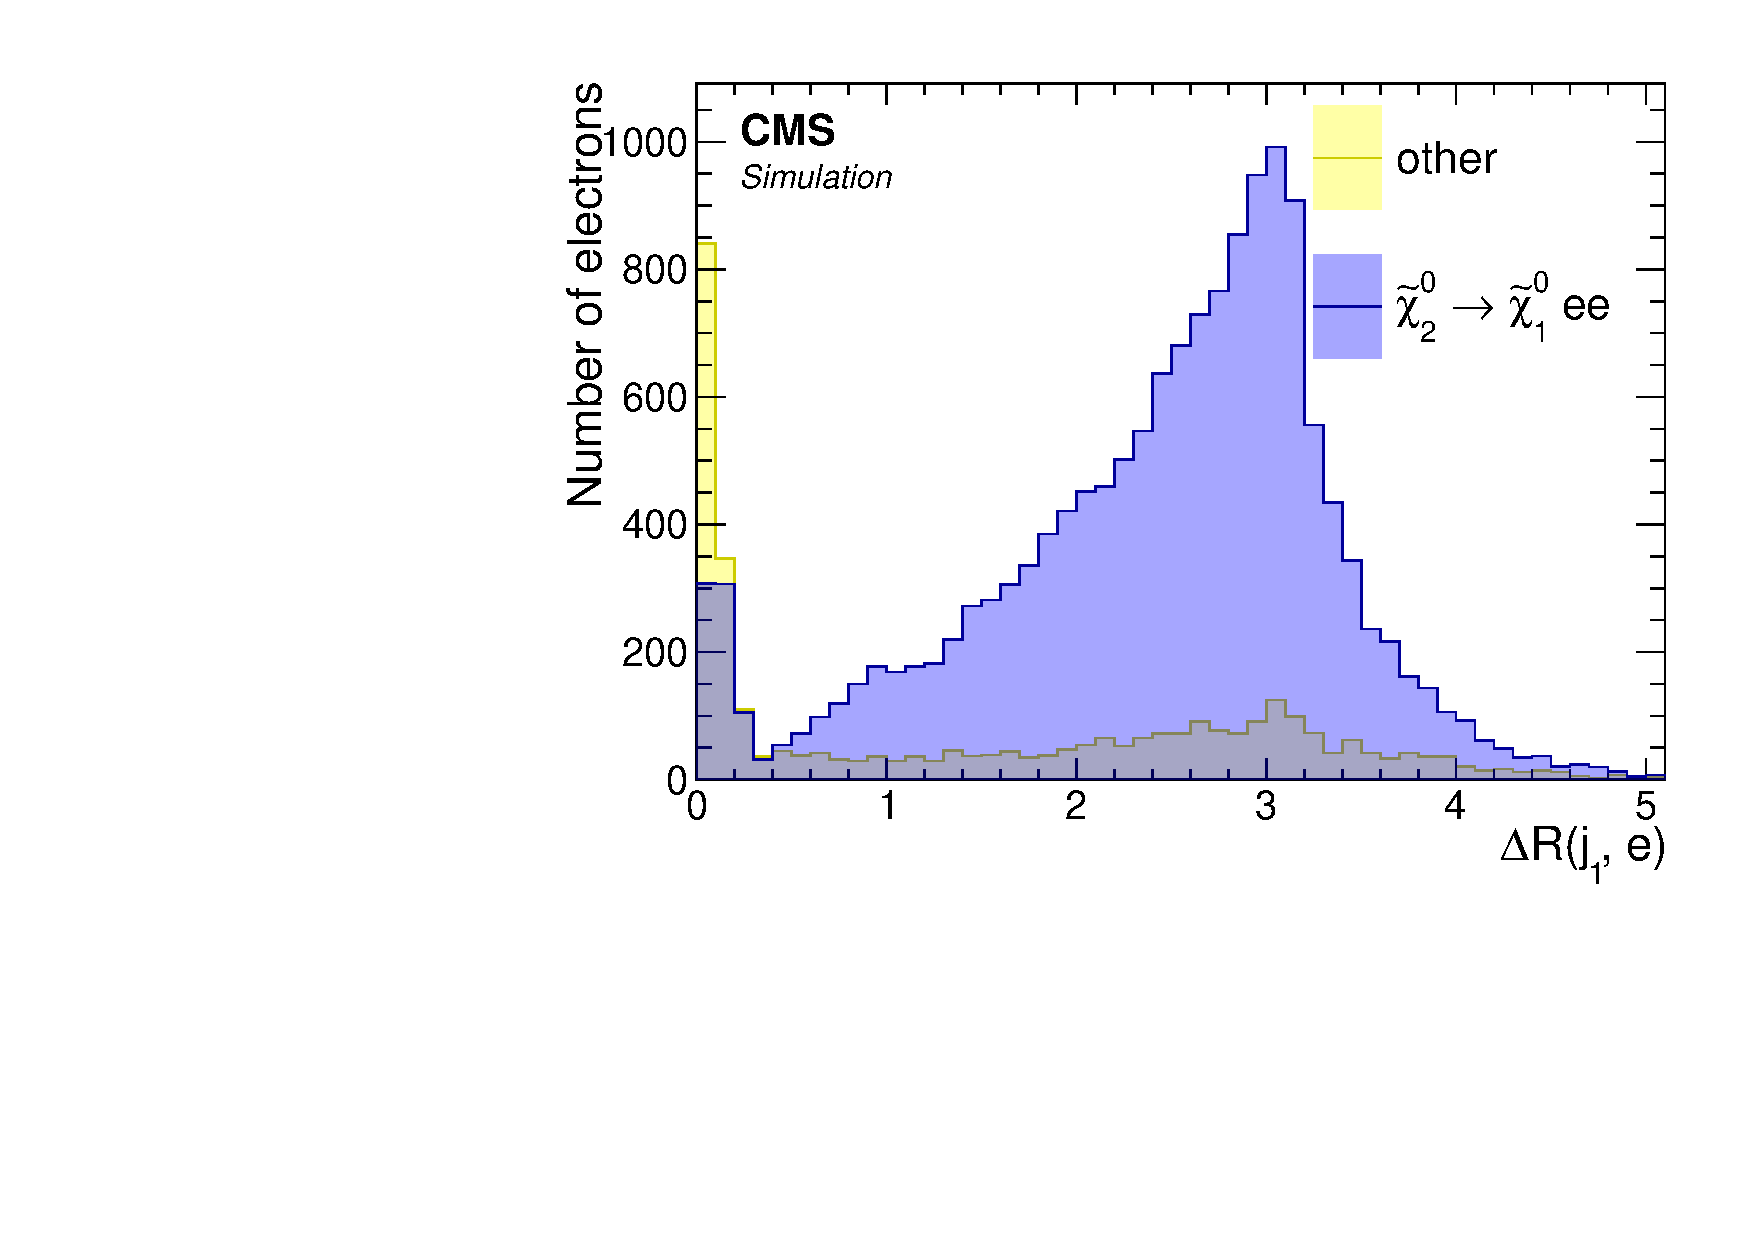
\includegraphics[width=0.48\linewidth]{plots/lepton_selection/lepton_selection_dm5p63/none_Electrons_rlj.pdf} \,
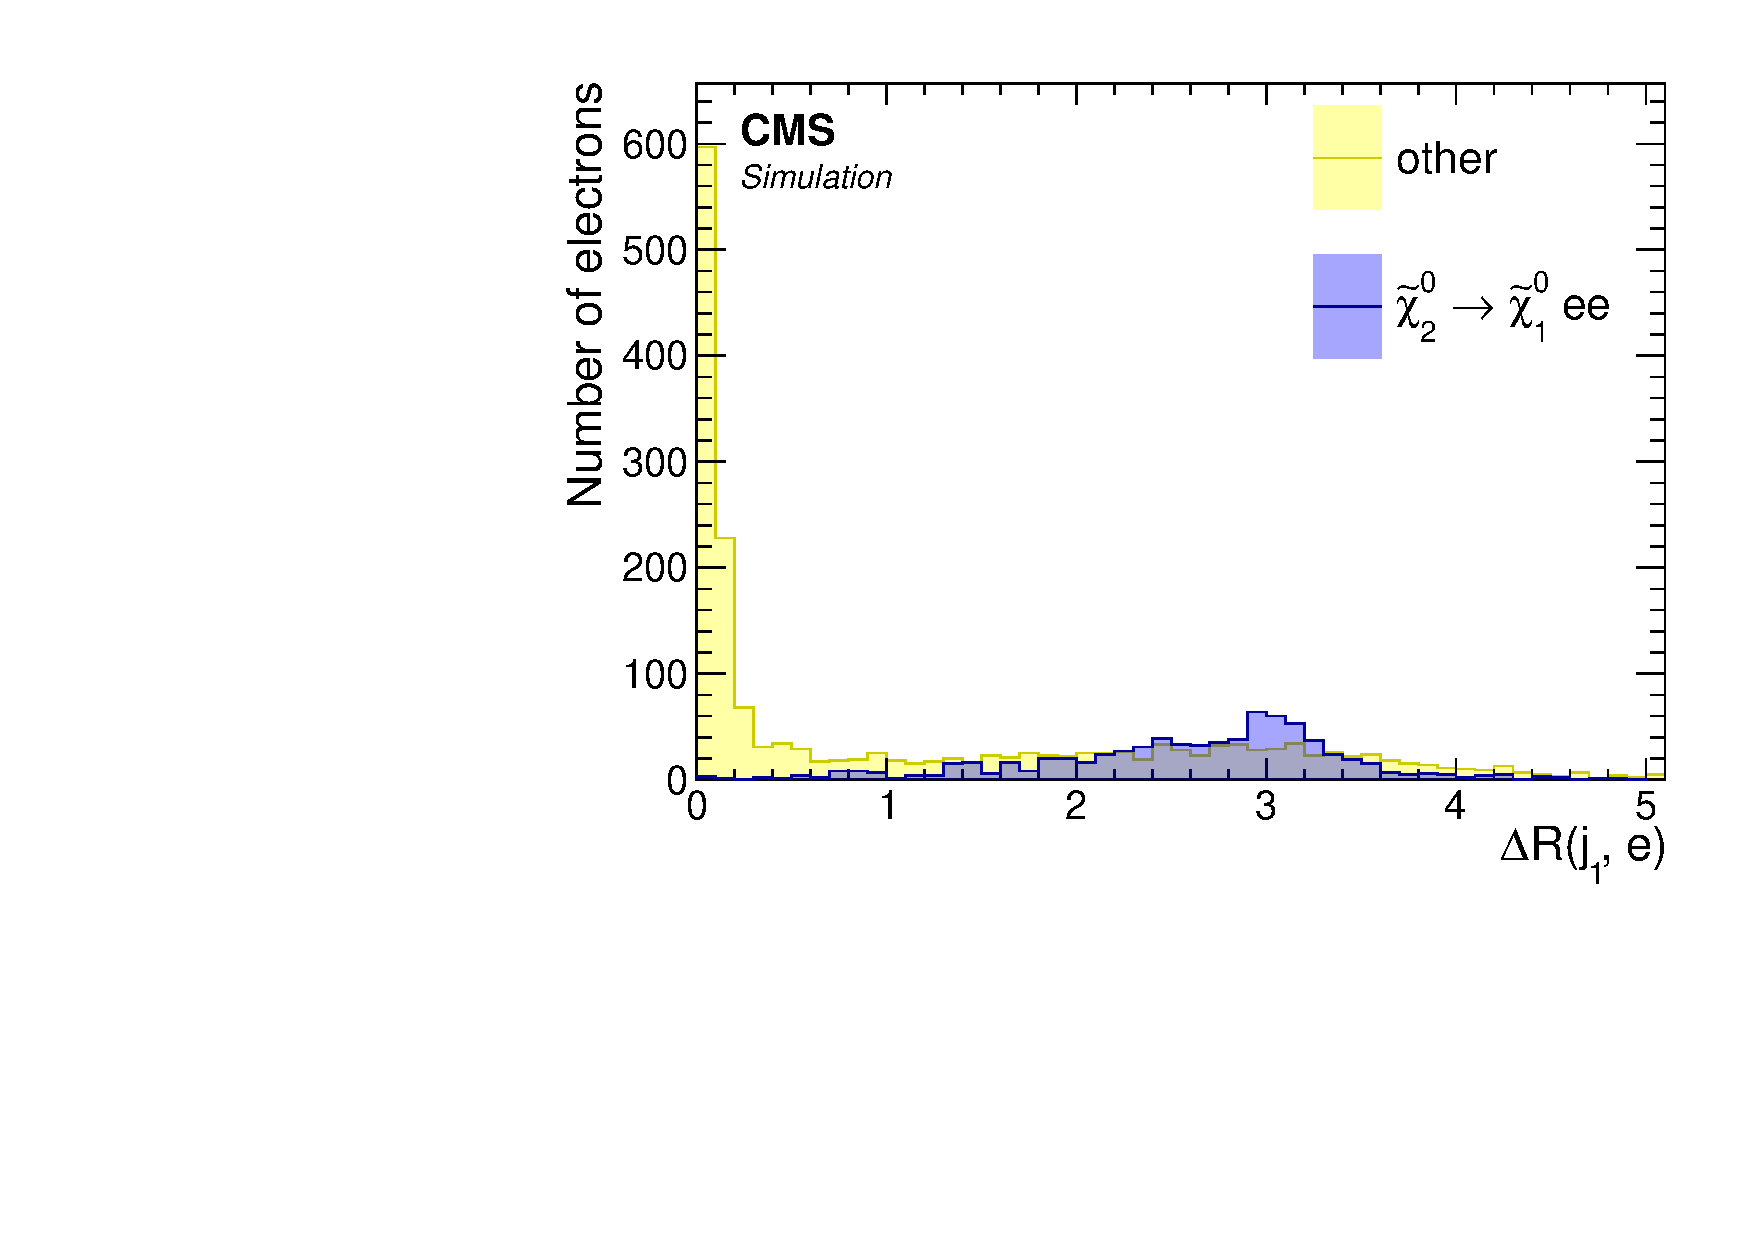
\includegraphics[width=0.48\linewidth]{plots/lepton_selection/lepton_selection_dm1p92/none_Electrons_rlj.pdf}  \\
\caption[Spatial seperation between reconstructed electrons and the leading jet $\DR(\jmath_1,\Pe)$]{Spatial seperation between reconstructed electrons with loose ID and the leading jet $\DR(\jmath_1,\Pe)$ for $\dm=5.63\GeV$ (left) and $\dm=1.92\GeV$ (right).}
\label{fig:electrons-dr-lj}
\end{figure}

There are two obvious features we can take from these plots. The first we have explored already in~\ref{sec:signal-signature}, namely, that probing lower \gls{dm} requires access to low \gls{pt} leptons, and since we are limited by a lower threshold of $\pt\geq 5\GeV$ on the electrons, that results in lower signal acceptance as can be seen by the difference between the high \gls{dm} and the low one. The second interesting feature that we can see, is that our signal electrons are located mainly outside of the leading jet. That is because the leading jet is usually an \gls{isr} jet which boosts the \tchiz system to away from it (back-to-back). We therefore make a cut $\DR(\jmath_1,\Pe)>0.4$.

Next we turn into the \gls{pt} distributions. We apply the previous cut of $\DR(\jmath_1,\Pe)>0.4$. As we've already seen in~\ref{sec:muon-eta-pt}, the \gls{pt} distribution depends strongly on \gls{dm}. Even though the distributions in~\ref{sec:muon-eta-pt} were plotted using generator level muons, the electrons distributions follow the same trend. We therefore need to make a choice about which \gls{dm} to favor, \ie, which \gls{dm} we want to be more sensitive to, and we choose the lower \gls{dm} case. Nonetheless we compare the two choices.

\begin{figure}[h]
\centering
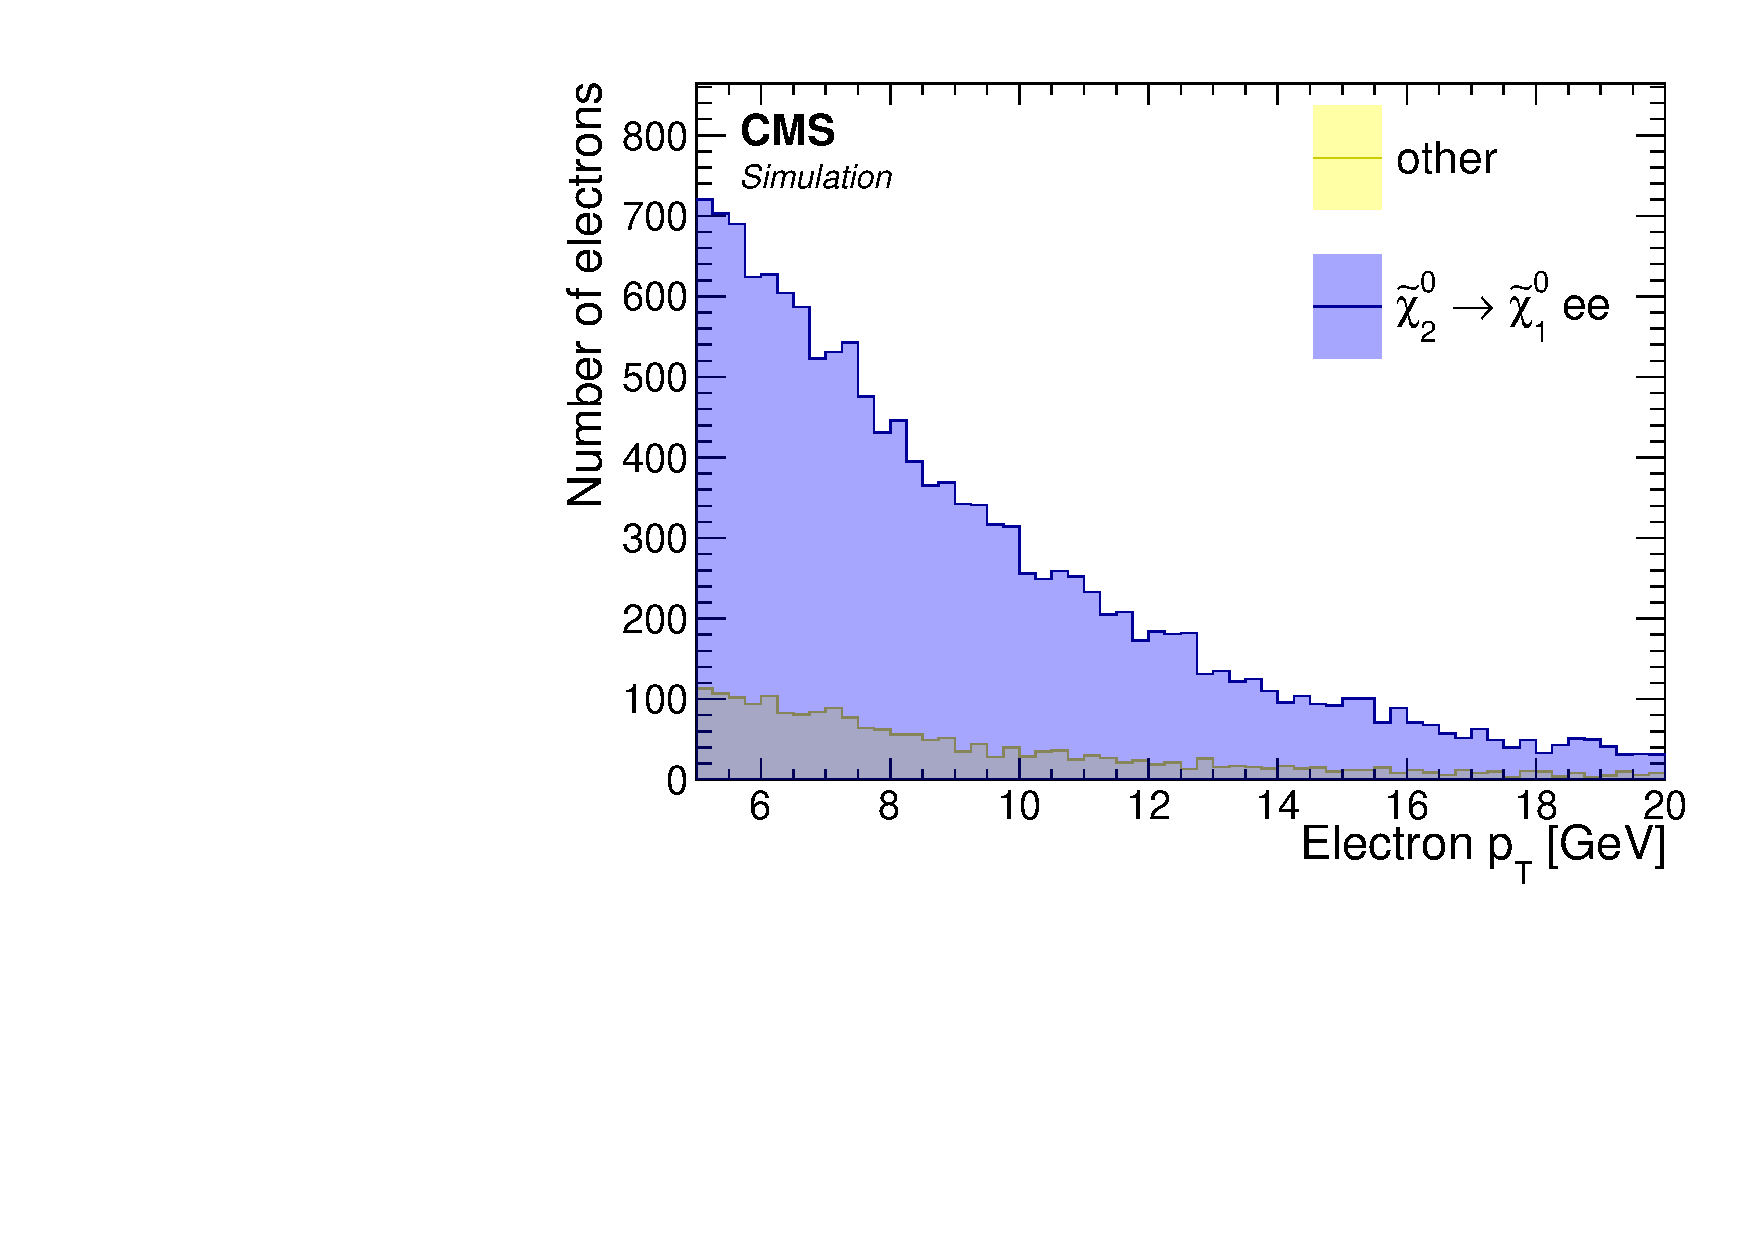
\includegraphics[width=0.48\linewidth]{plots/lepton_selection/lepton_selection_dm5p63/none_Electrons_pt.pdf} \,
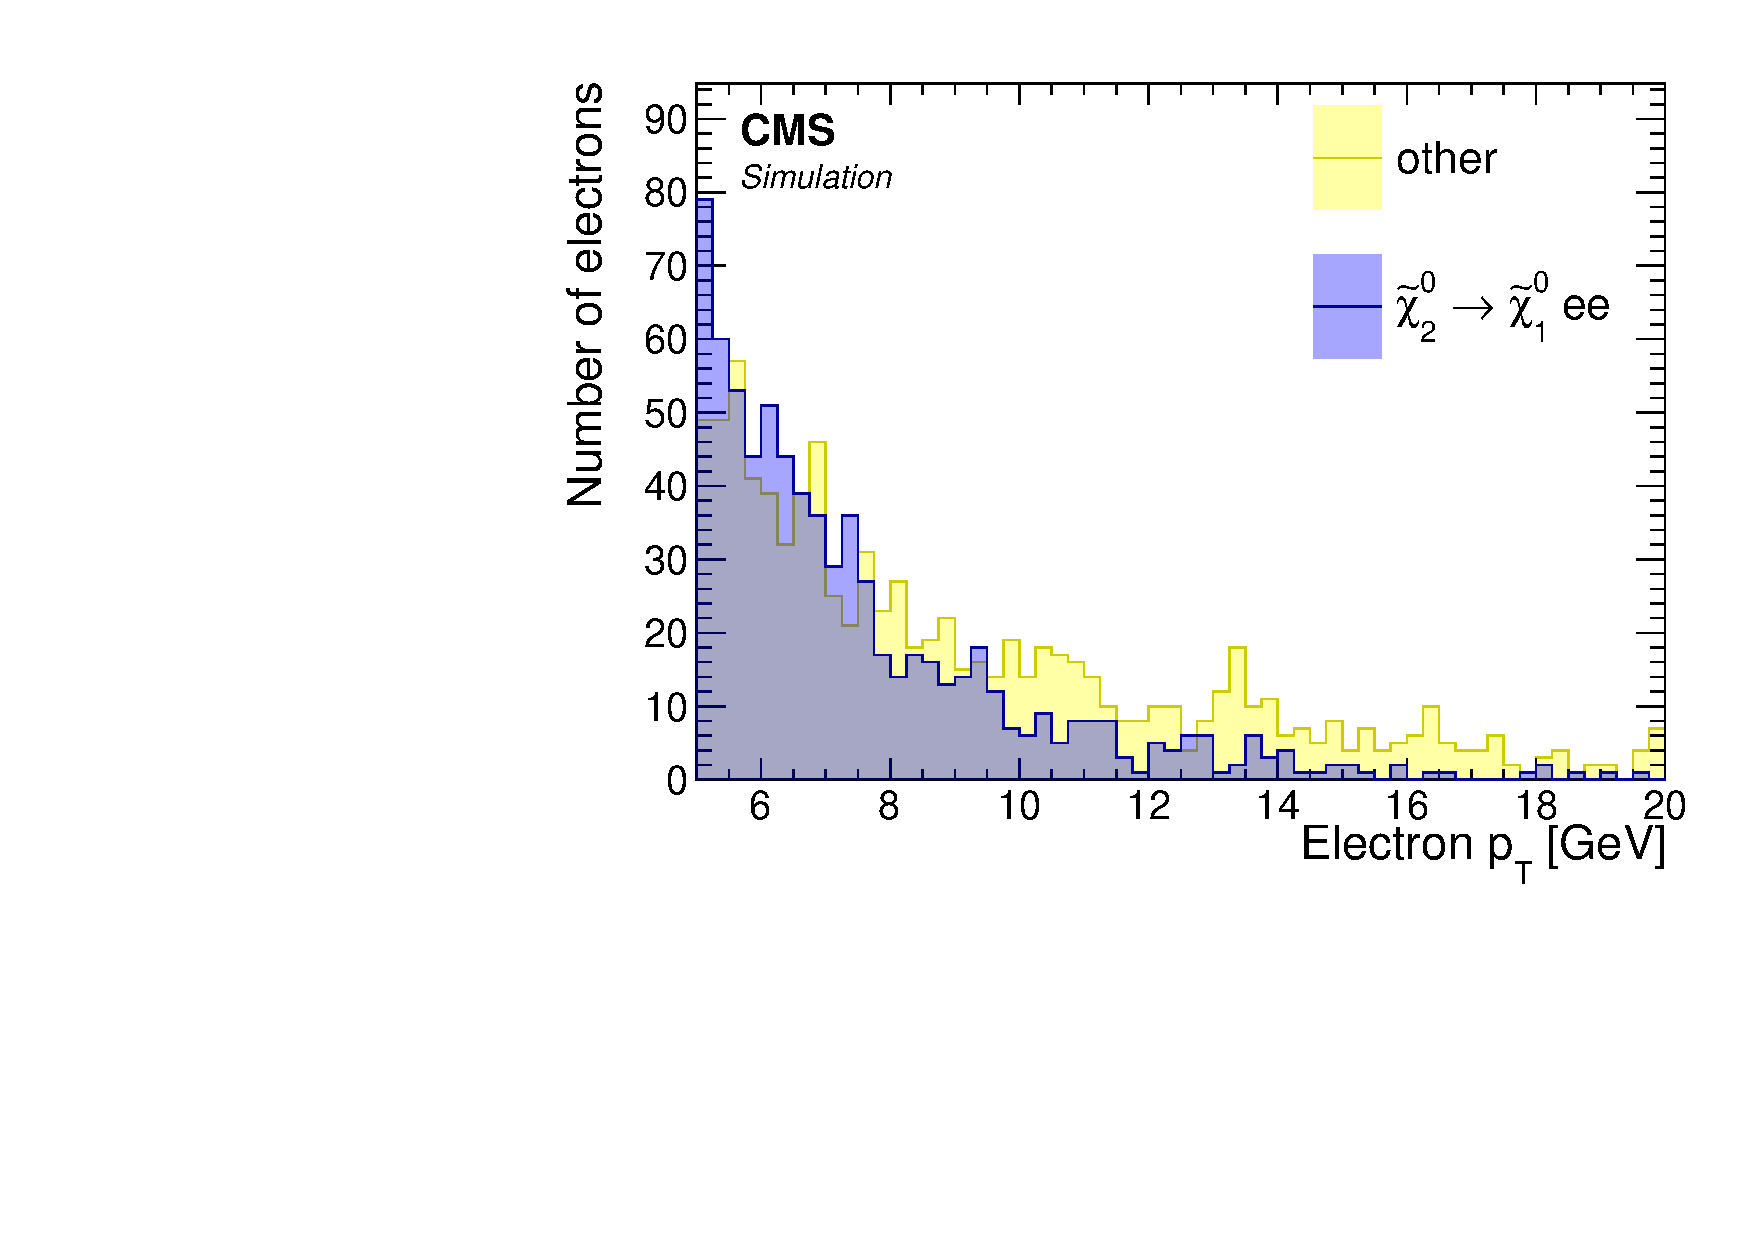
\includegraphics[width=0.48\linewidth]{plots/lepton_selection/lepton_selection_dm1p92/none_Electrons_pt.pdf}  \\
\caption[\pt distribution of reconstructed electrons with loose ID]{ \pt distribution of reconstructed electrons with loose ID for $\dm=5.63\GeV$ (left) and $\dm=1.92\GeV$ (right). Cut of $\DR(\jmath_1,\Pe)>0.4$ applied.}
\label{fig:electrons-selection-pt}
\end{figure}

We can see, as expected, that the \pt distribution  of the electrons fall more rapidly for the low \dm case. We observe that there are hardly any electrons surviving above $15\GeV$, and therefore we choose to make a cut of $\pt<15\GeV$.

It interesting to look at the $\eta$ distribution after the previous cuts to get a better sense of where most of the non-signal electrons are stil coming from.

\begin{figure}[h]
\centering
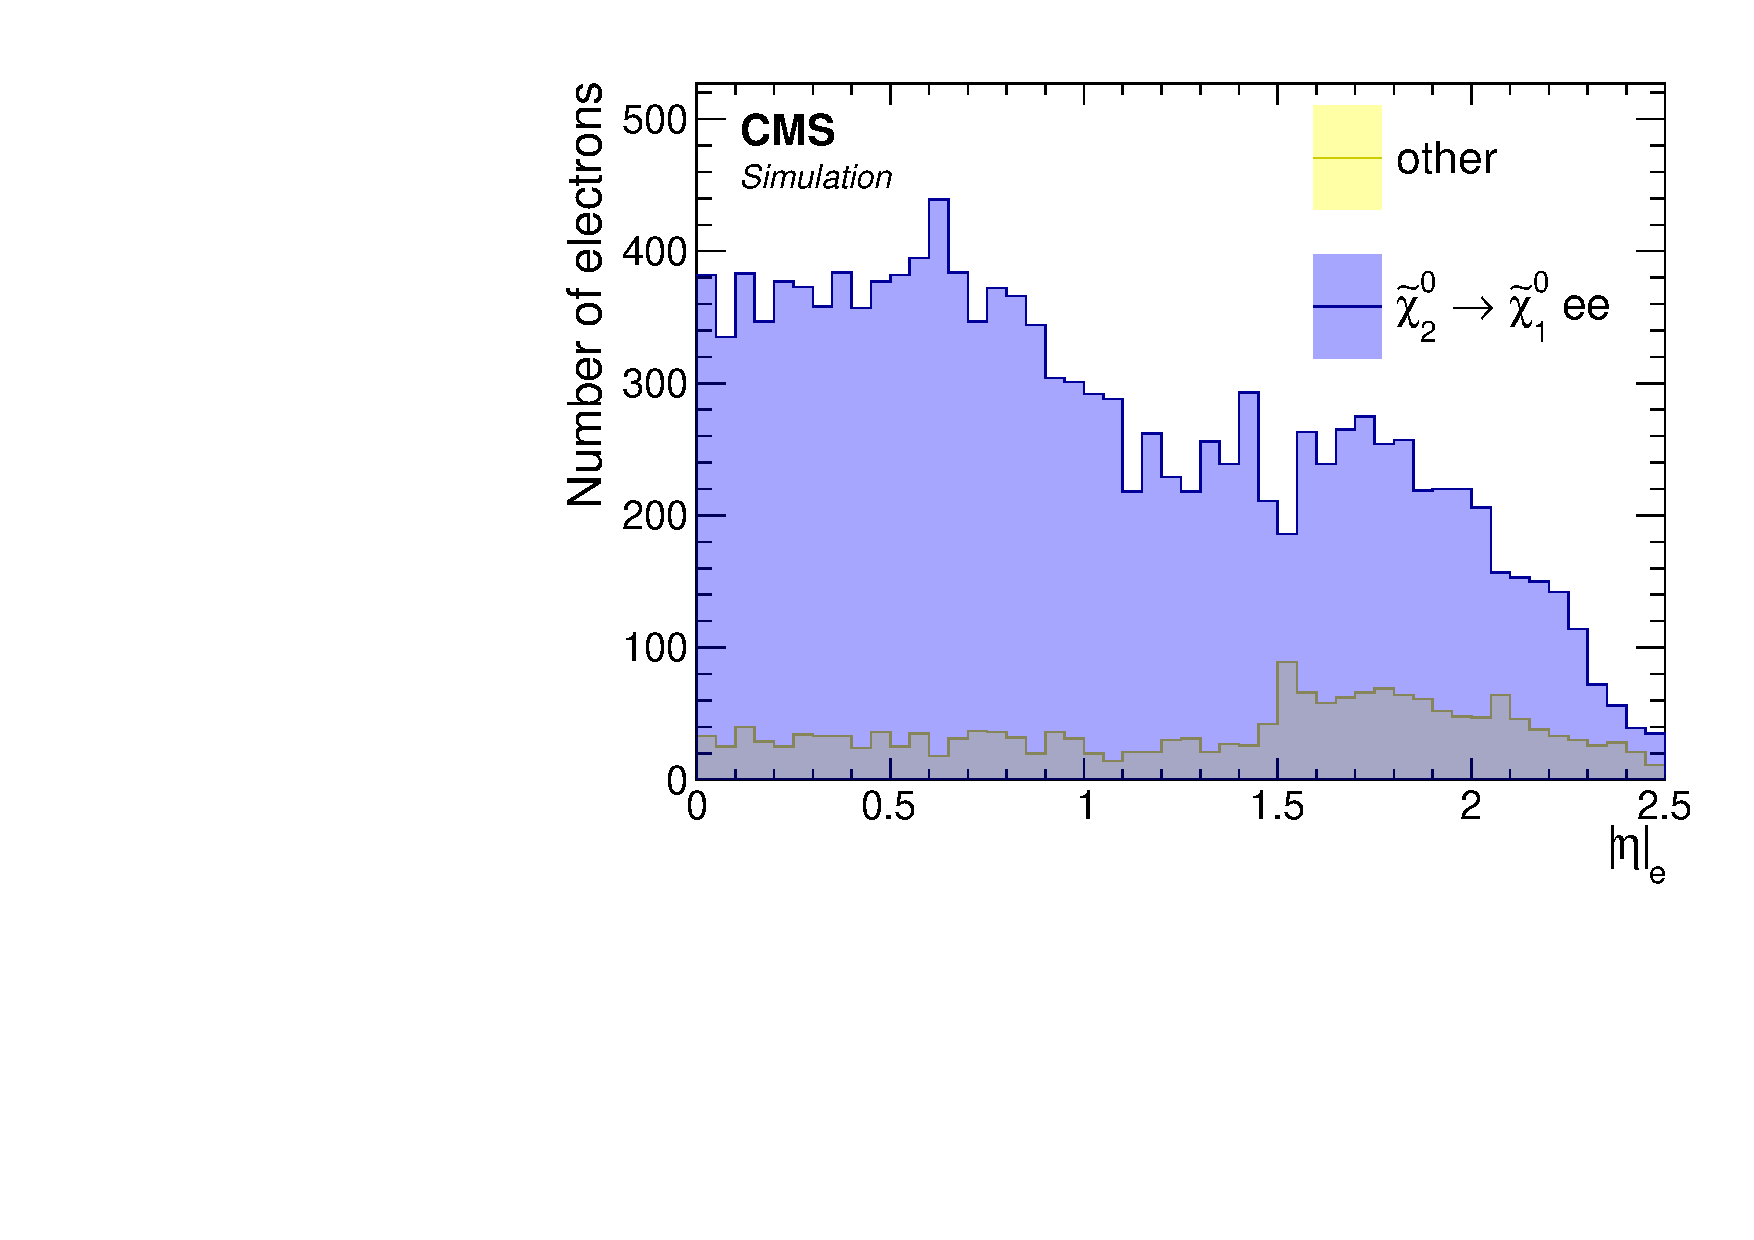
\includegraphics[width=0.48\linewidth]{plots/lepton_selection/lepton_selection_dm5p63/none_Electrons_eta.pdf} \,
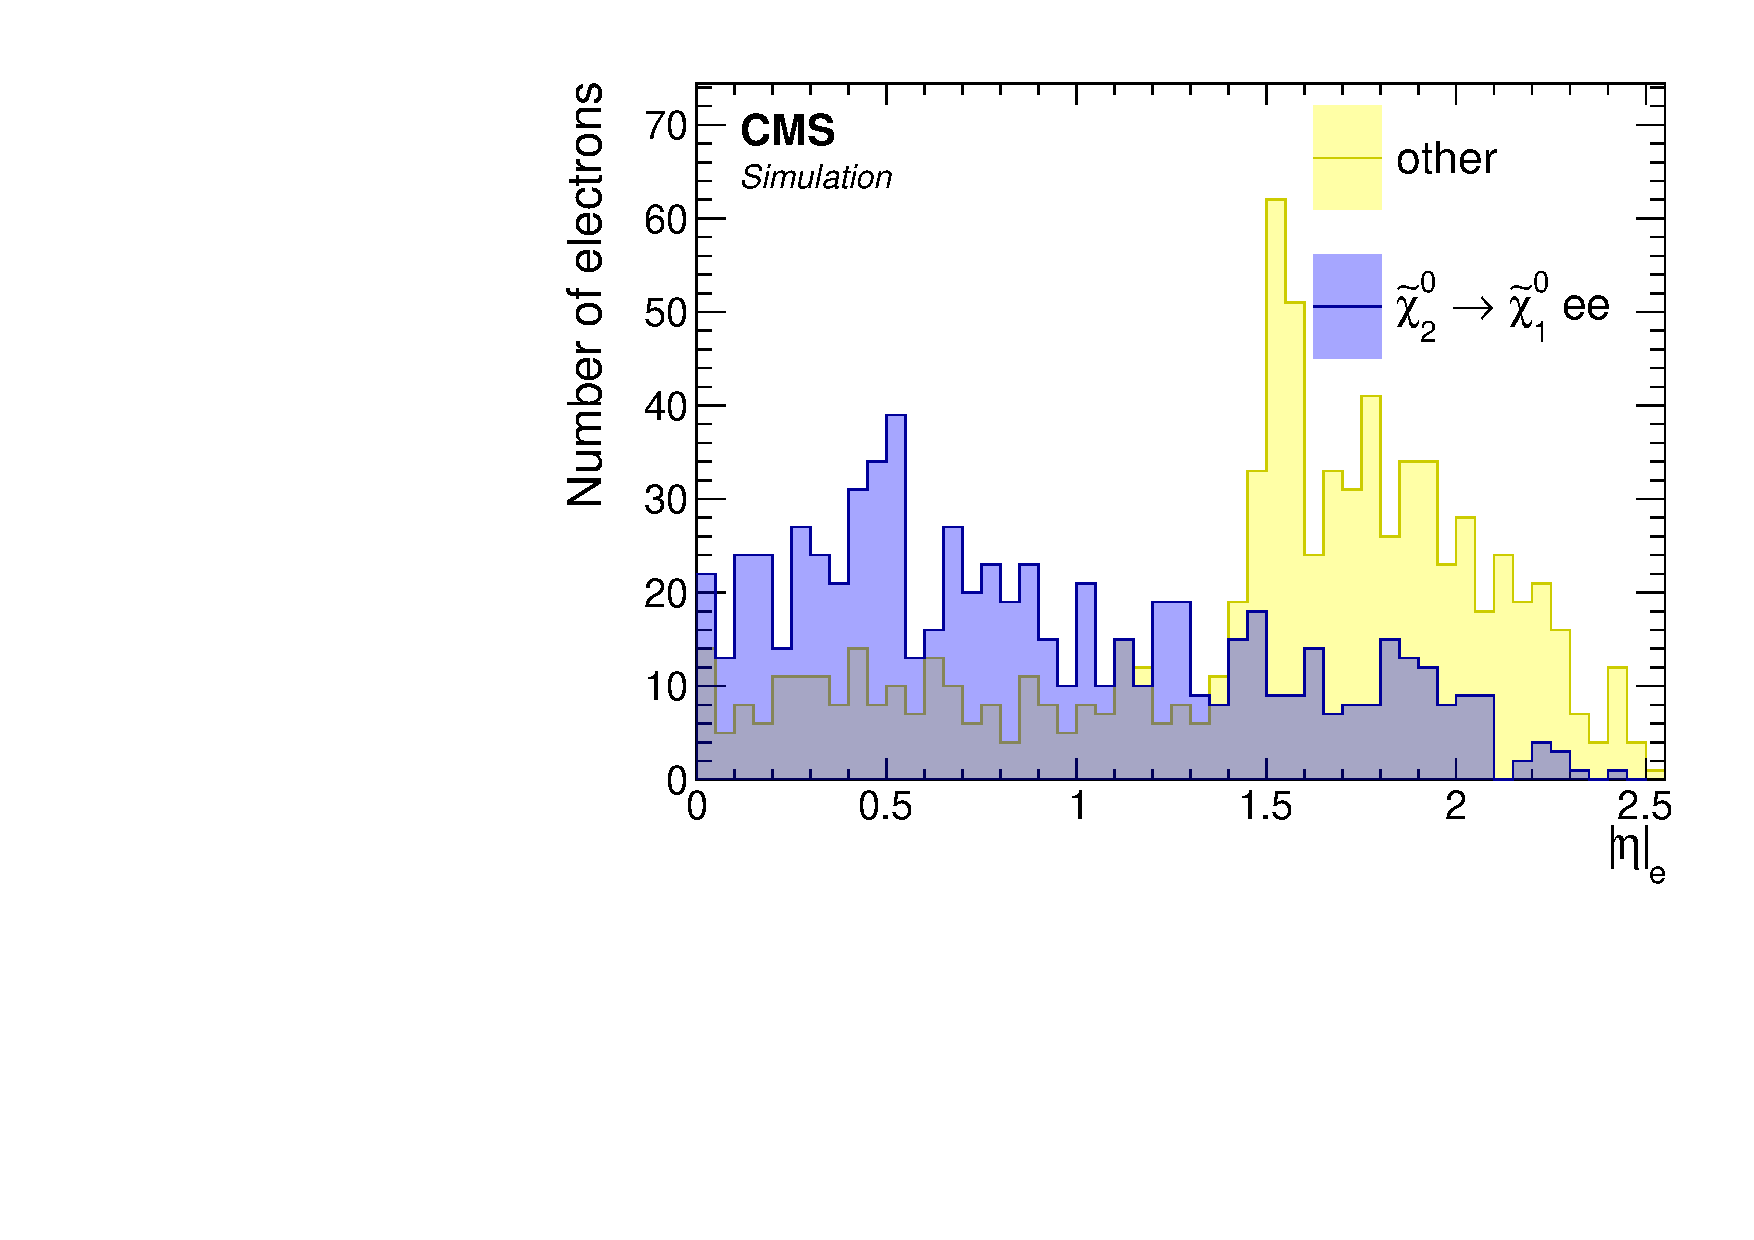
\includegraphics[width=0.48\linewidth]{plots/lepton_selection/lepton_selection_dm1p92/none_Electrons_eta.pdf}  \\
\caption[\abs{\eta} distribution of reconstructed electrons with loose ID]{ \abs{\eta} distribution of reconstructed electrons with loose ID for $\dm=5.63\GeV$ (left) and $\dm=1.92\GeV$ (right). Cuts of $\DR(\jmath_1,\Pe)>0.4$ and $\pt<15\GeV$ are applied.}
\label{fig:electrons-selection-eta}
\end{figure}

In the case of $\dm=1.92\GeV$,  we can clearly see how worse the endcaps of the \gls{ecal} are performing in comparison with the barrel ($\abs{\eta}<1.48$). The transition is clearly visible through a sharp drop in purity at the transition. It is worse for low-\pt electrons than higher-\pt ones.

We would like to see if requiring a tighter working point for the electron-identification is beneficial. The working point used in the previous distributions is loose. We look turn now to check the effects of requiring either a medium working point, or a tight one. We plot two bins labeled \emph{fail} and \emph{pass}, which correspond to whether the electron passes or failed the identification criteria of a medium or tight working points.

\begin{figure}[h]
\centering
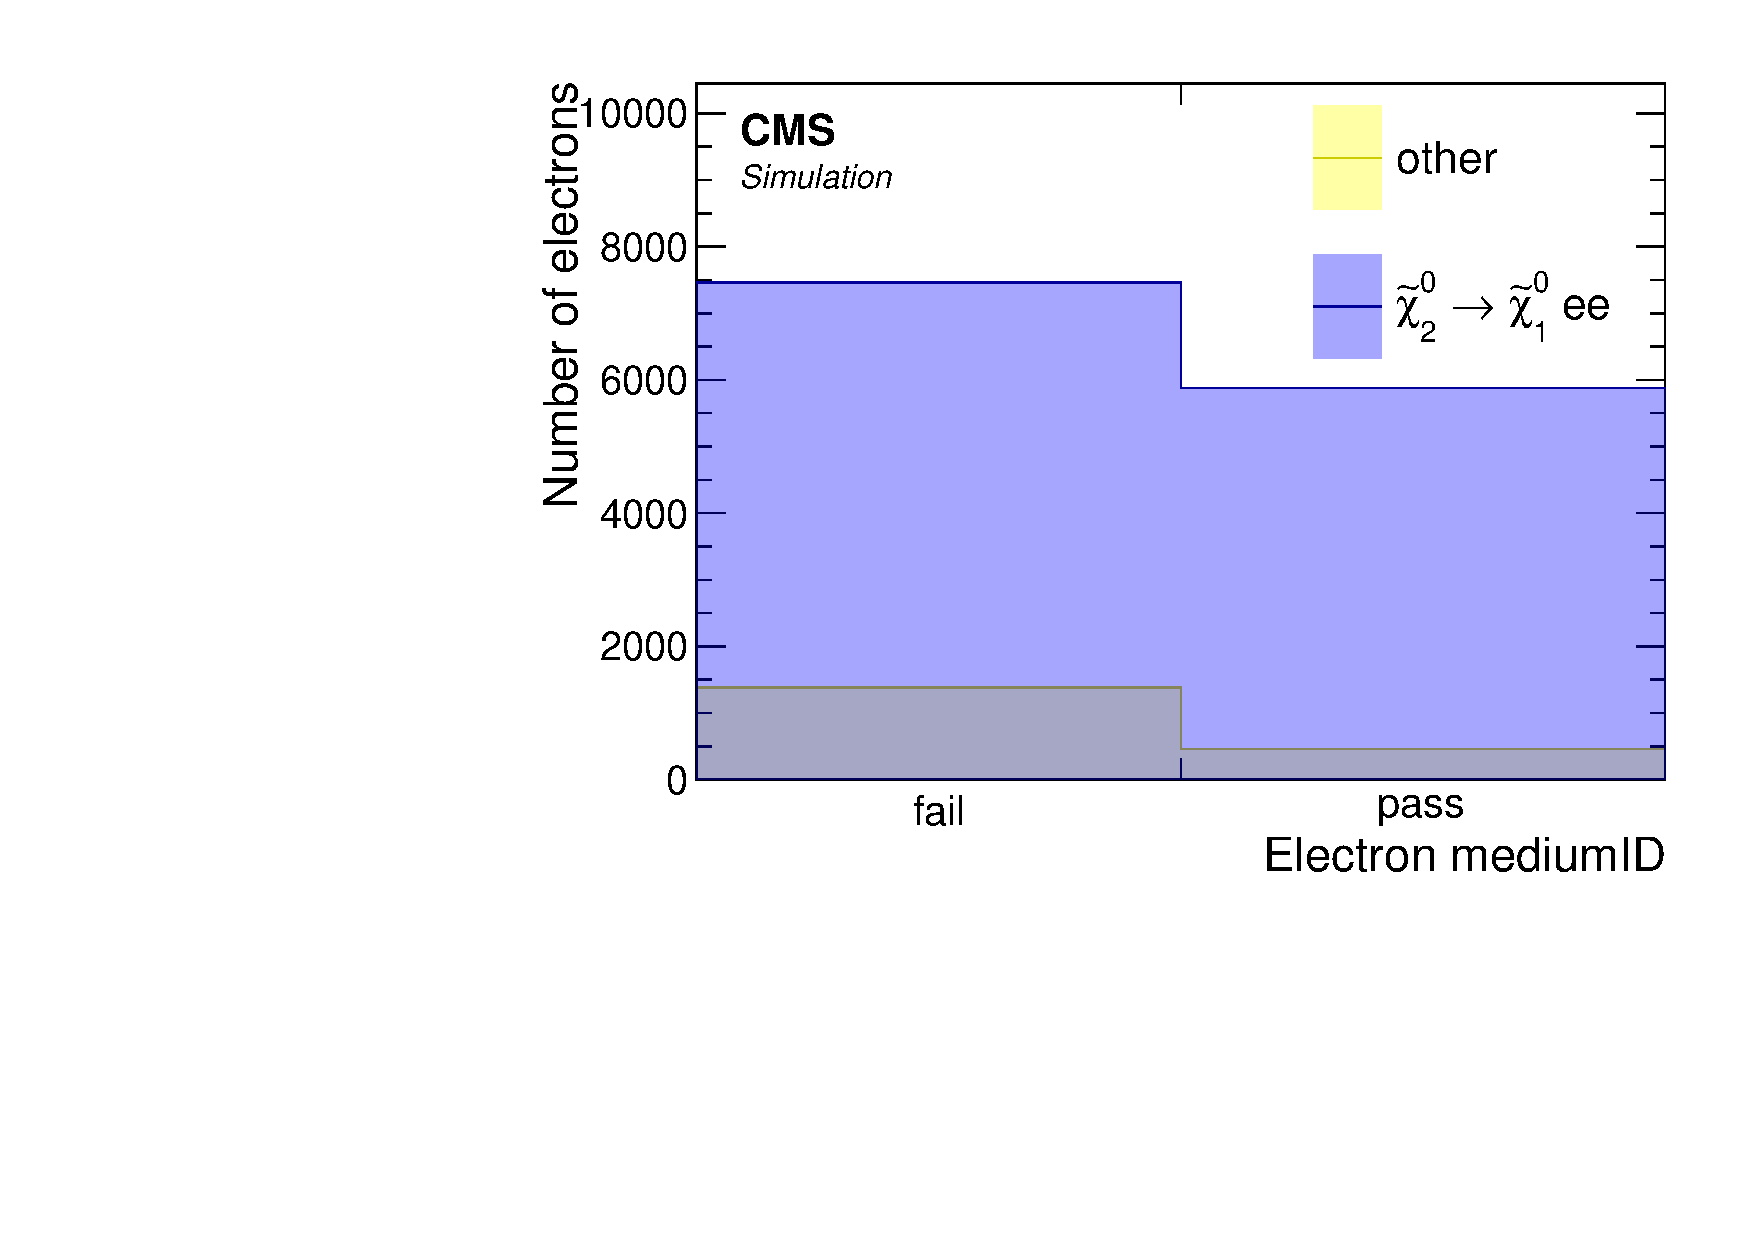
\includegraphics[width=0.48\linewidth]{plots/lepton_selection/lepton_selection_dm5p63/none_Electrons_medium.pdf} \,
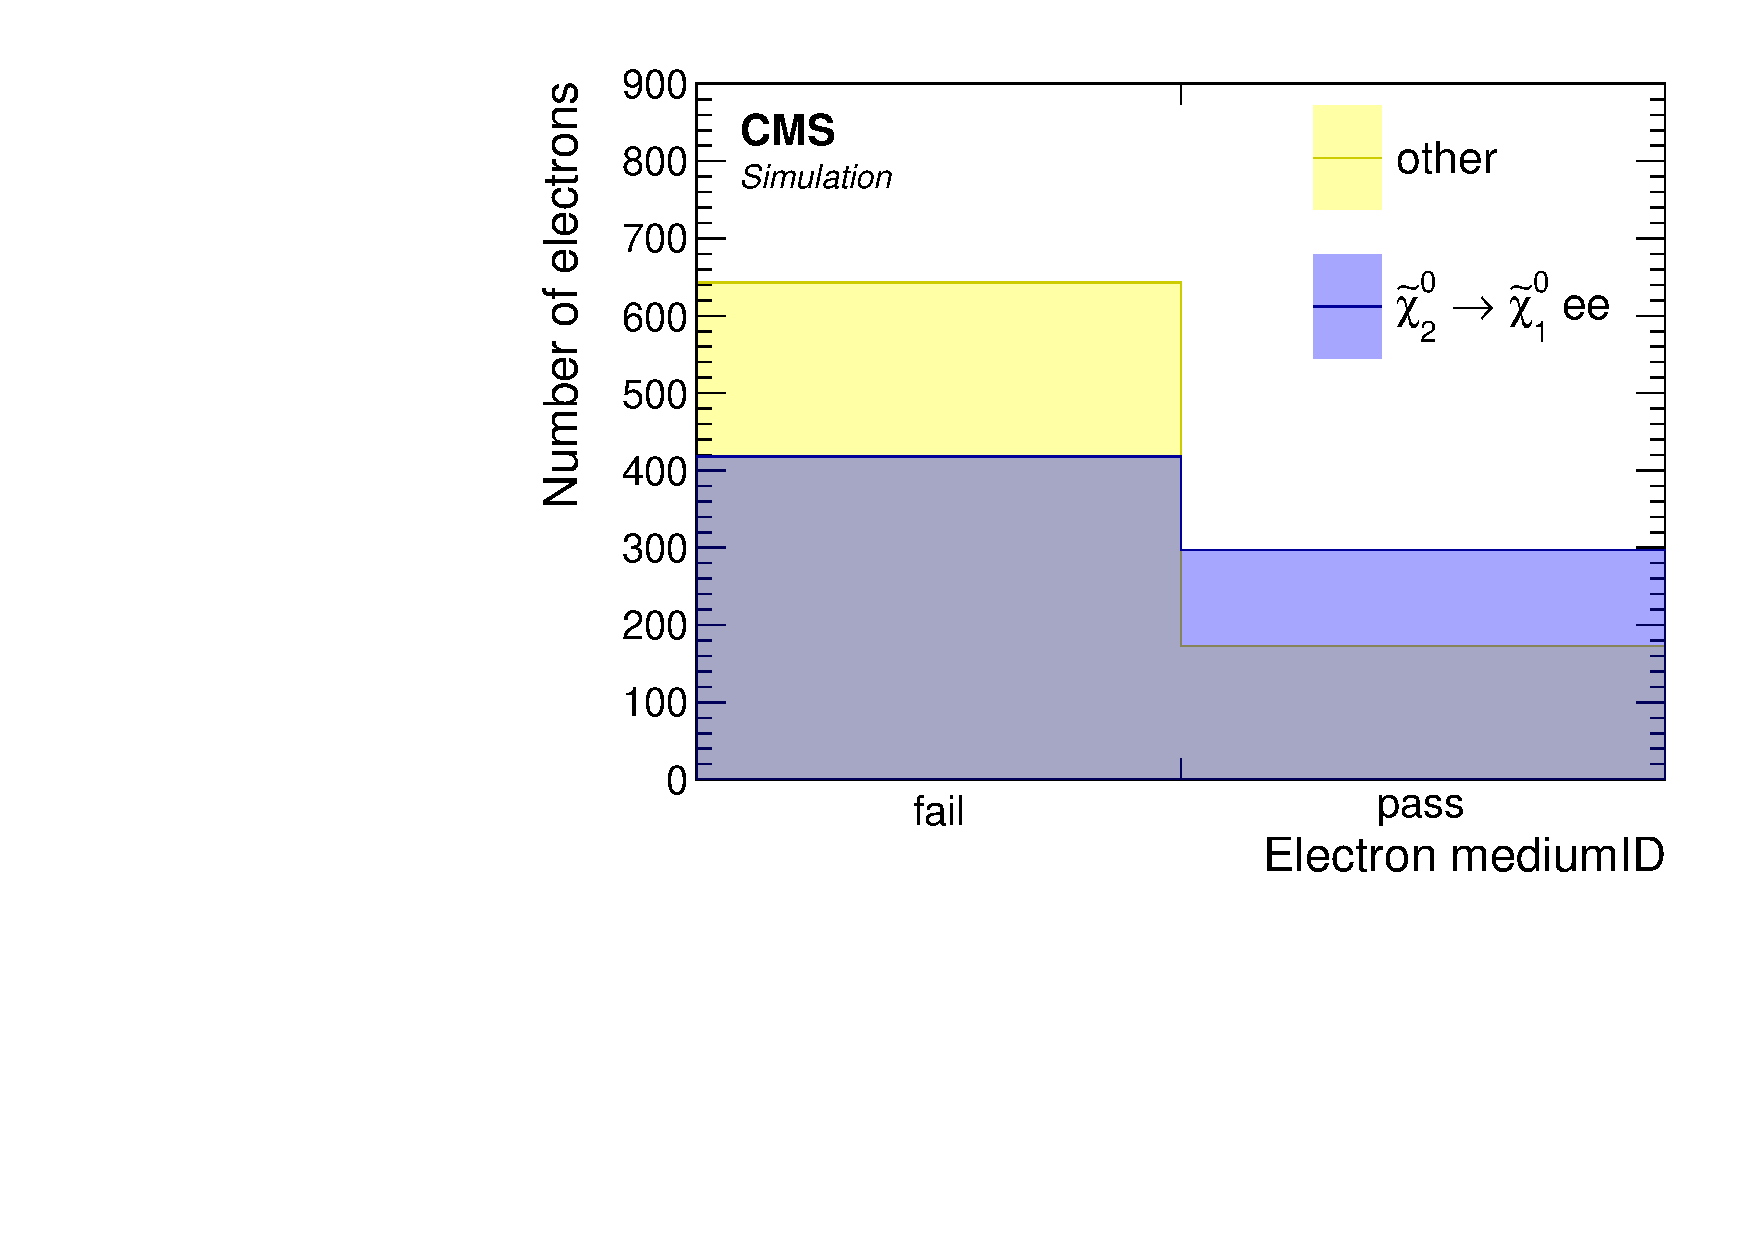
\includegraphics[width=0.48\linewidth]{plots/lepton_selection/lepton_selection_dm1p92/none_Electrons_medium.pdf}  \\
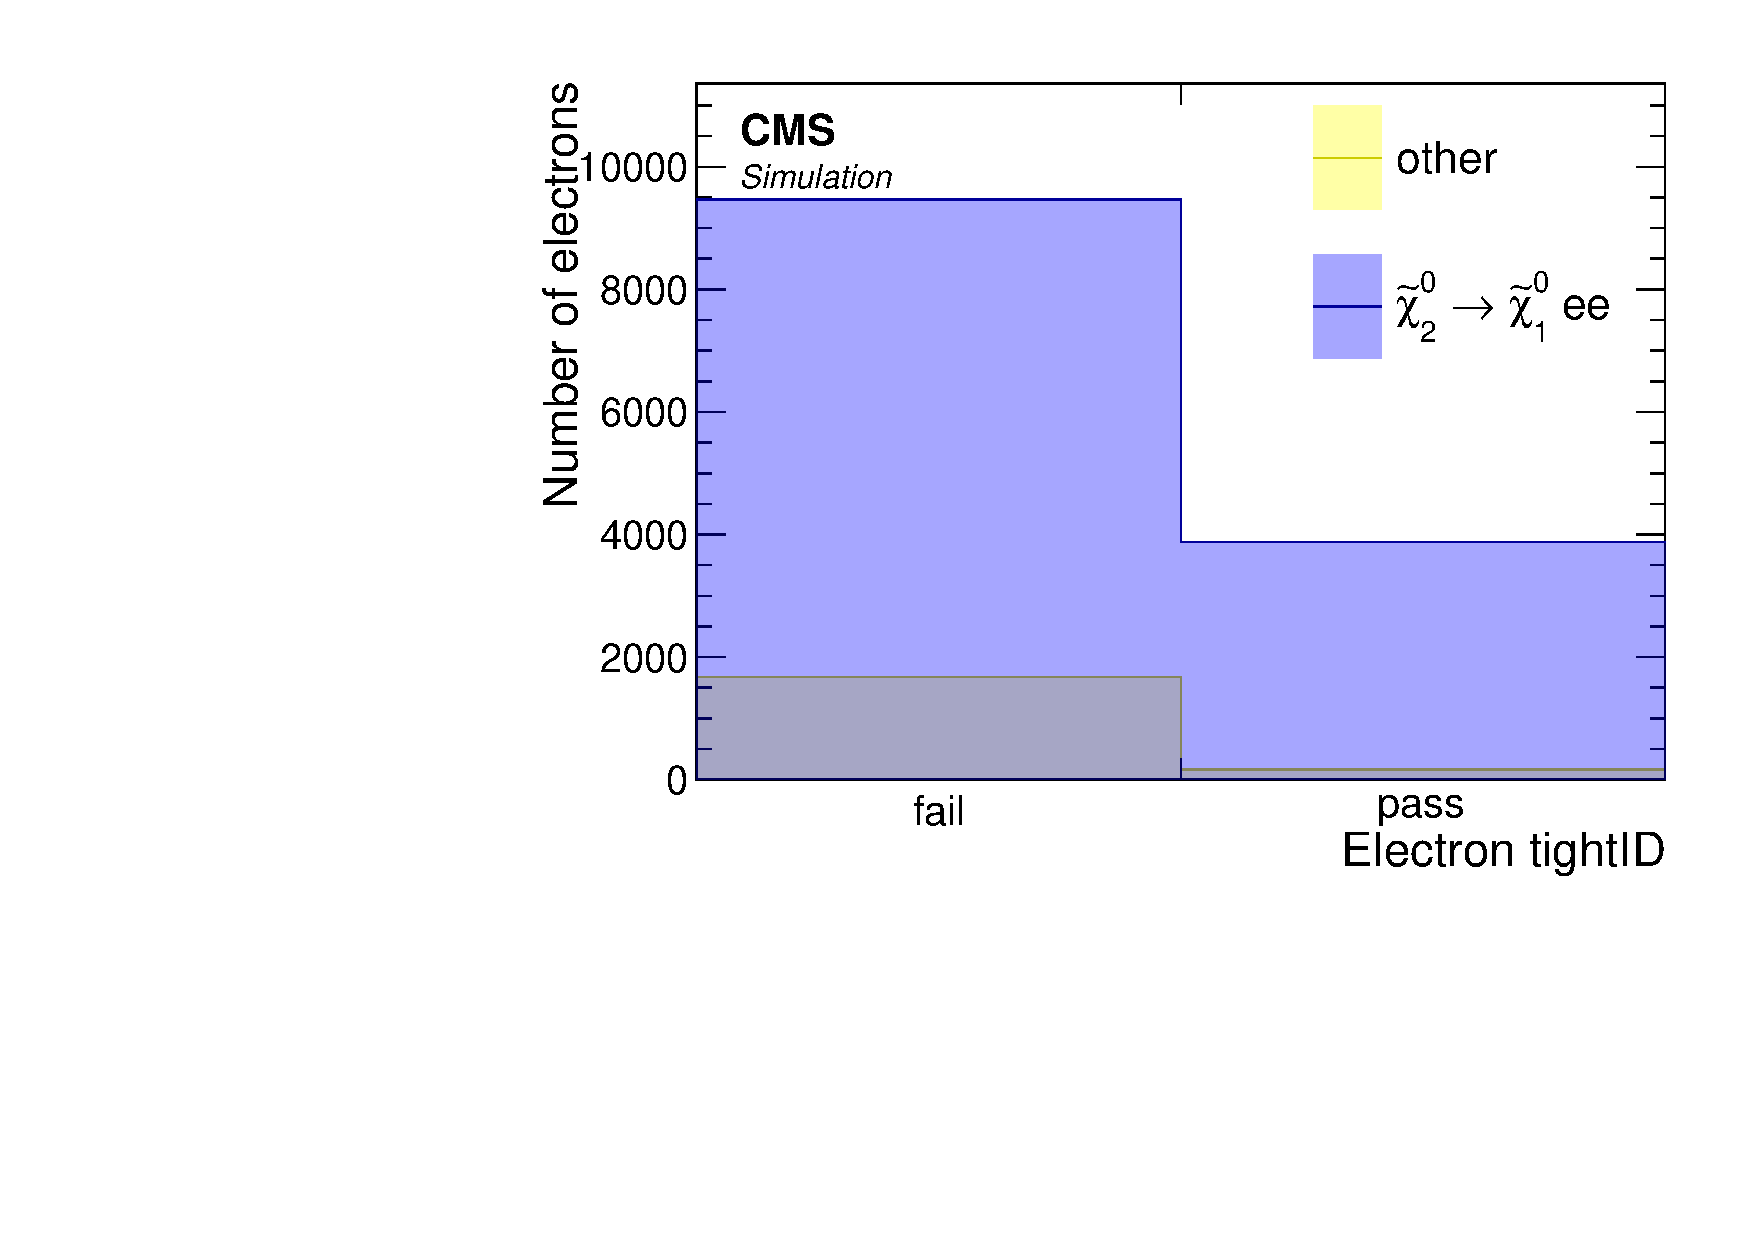
\includegraphics[width=0.48\linewidth]{plots/lepton_selection/lepton_selection_dm5p63/none_Electrons_tight.pdf} \,
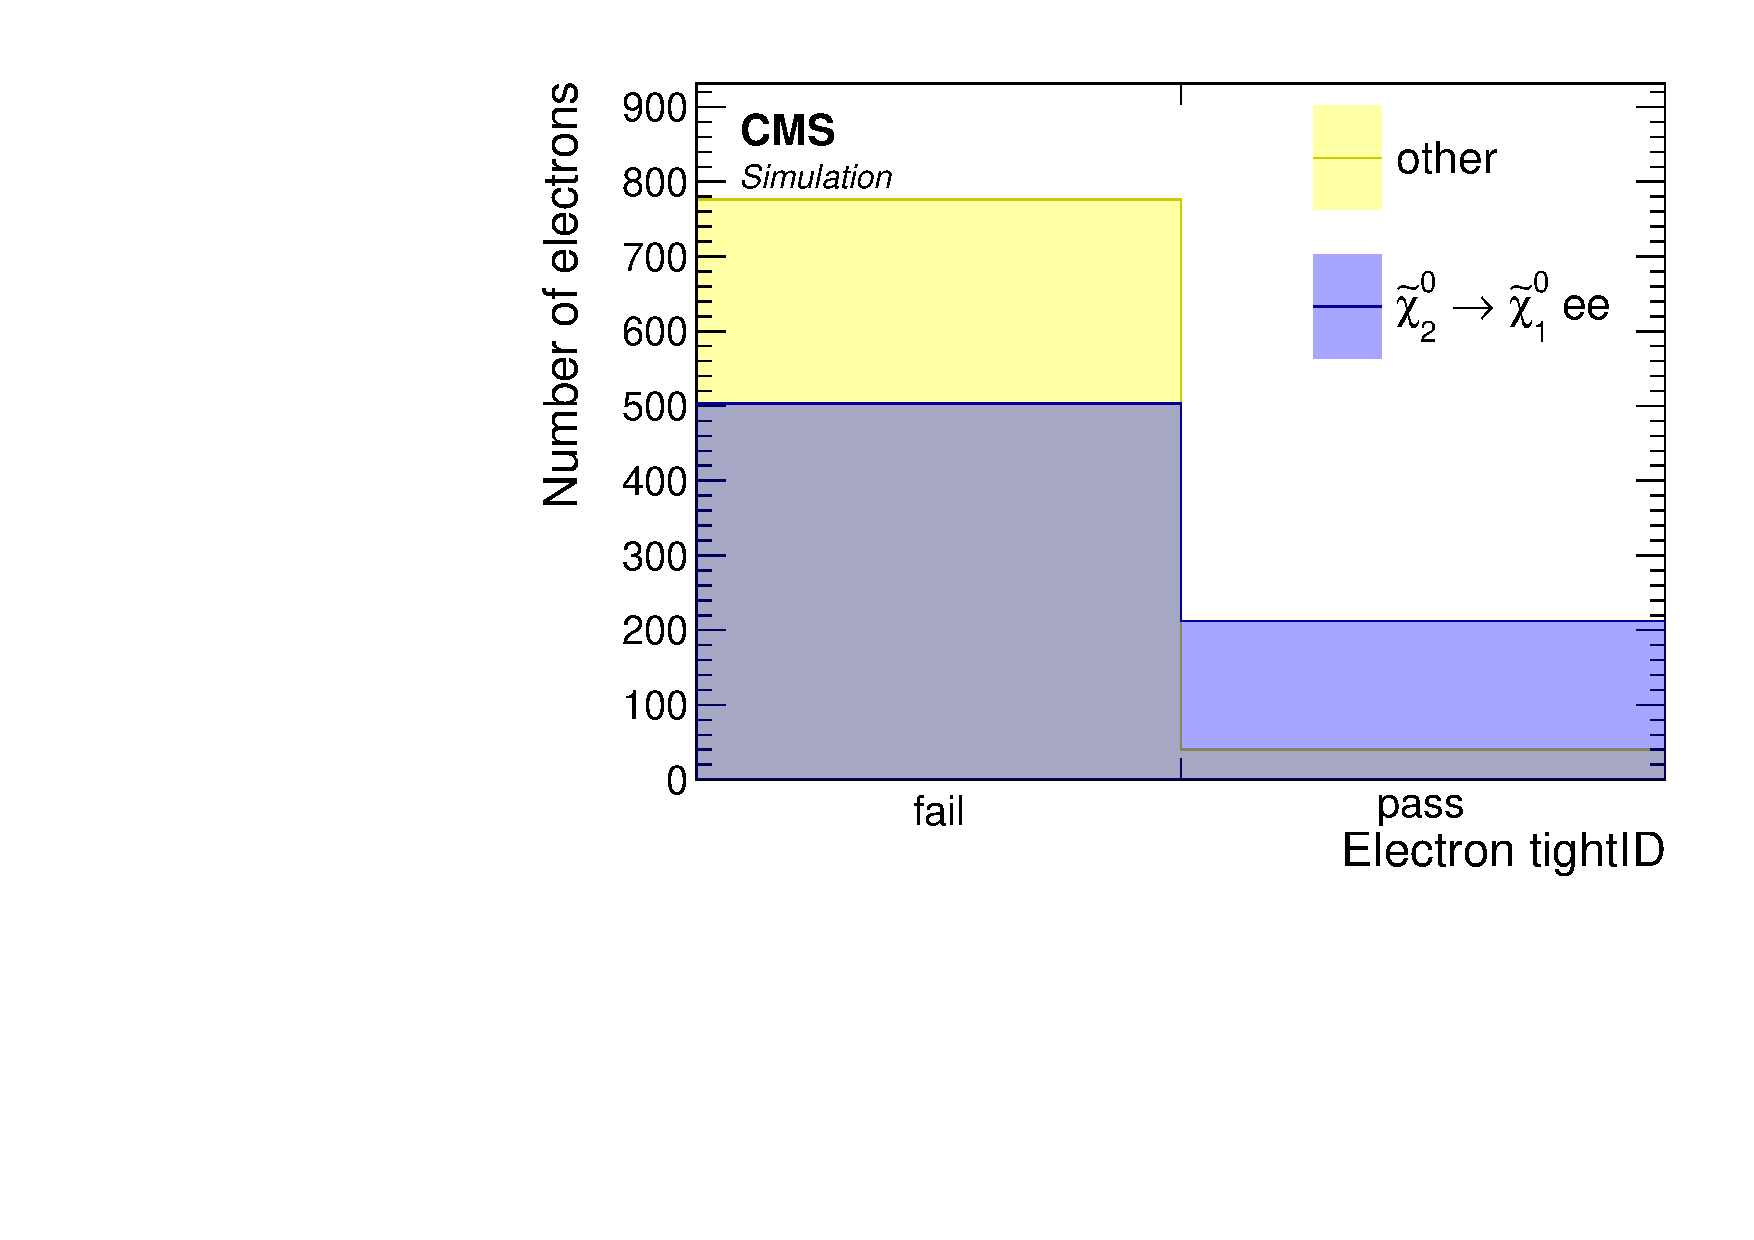
\includegraphics[width=0.48\linewidth]{plots/lepton_selection/lepton_selection_dm1p92/none_Electrons_tight.pdf}  \\
\caption[medium and tight ID working points distribution of reconstructed electrons]{Medium (top) and tight (bottom) ID working points distributions of reconstructed electrons for $\dm=5.63\GeV$ (left) and $\dm=1.92\GeV$ (right). Cuts of $\DR(\jmath_1,\Pe)>0.4$ and $\pt<15\GeV$ are applied.}
\label{fig:electrons-selection-id}
\end{figure}

To select a medium or a tight working point is equivalent to choosing the relevant right \emph{pass} bin (top for medium, bottom for tight), and rejecting the electrons on the left \emph{fail} bin. We see that although we reject considerable amount of non-signal electrons in the low \dm case by picking either a medium or tight working points, we also loose quite a lot of signal electrons as well. In other words, these selections are very not efficient and will result in low signal acceptance. We therefore decide to use a loose working point for the electrons. We will see that we can still purify the electron selection by relying on isolation instead. We fully discuss and describe our jet-isolation in~\ref{sec:isolation}, but here for the sake of completeness we look at its effect on the purity of the electrons. We compare our custom jet-isolation to the standard definition of lepton isolation, which does not take into account the possibility that two electrons can be produced close to each other (small \DR), as is the case in our signal.

\begin{figure}[h]
\centering
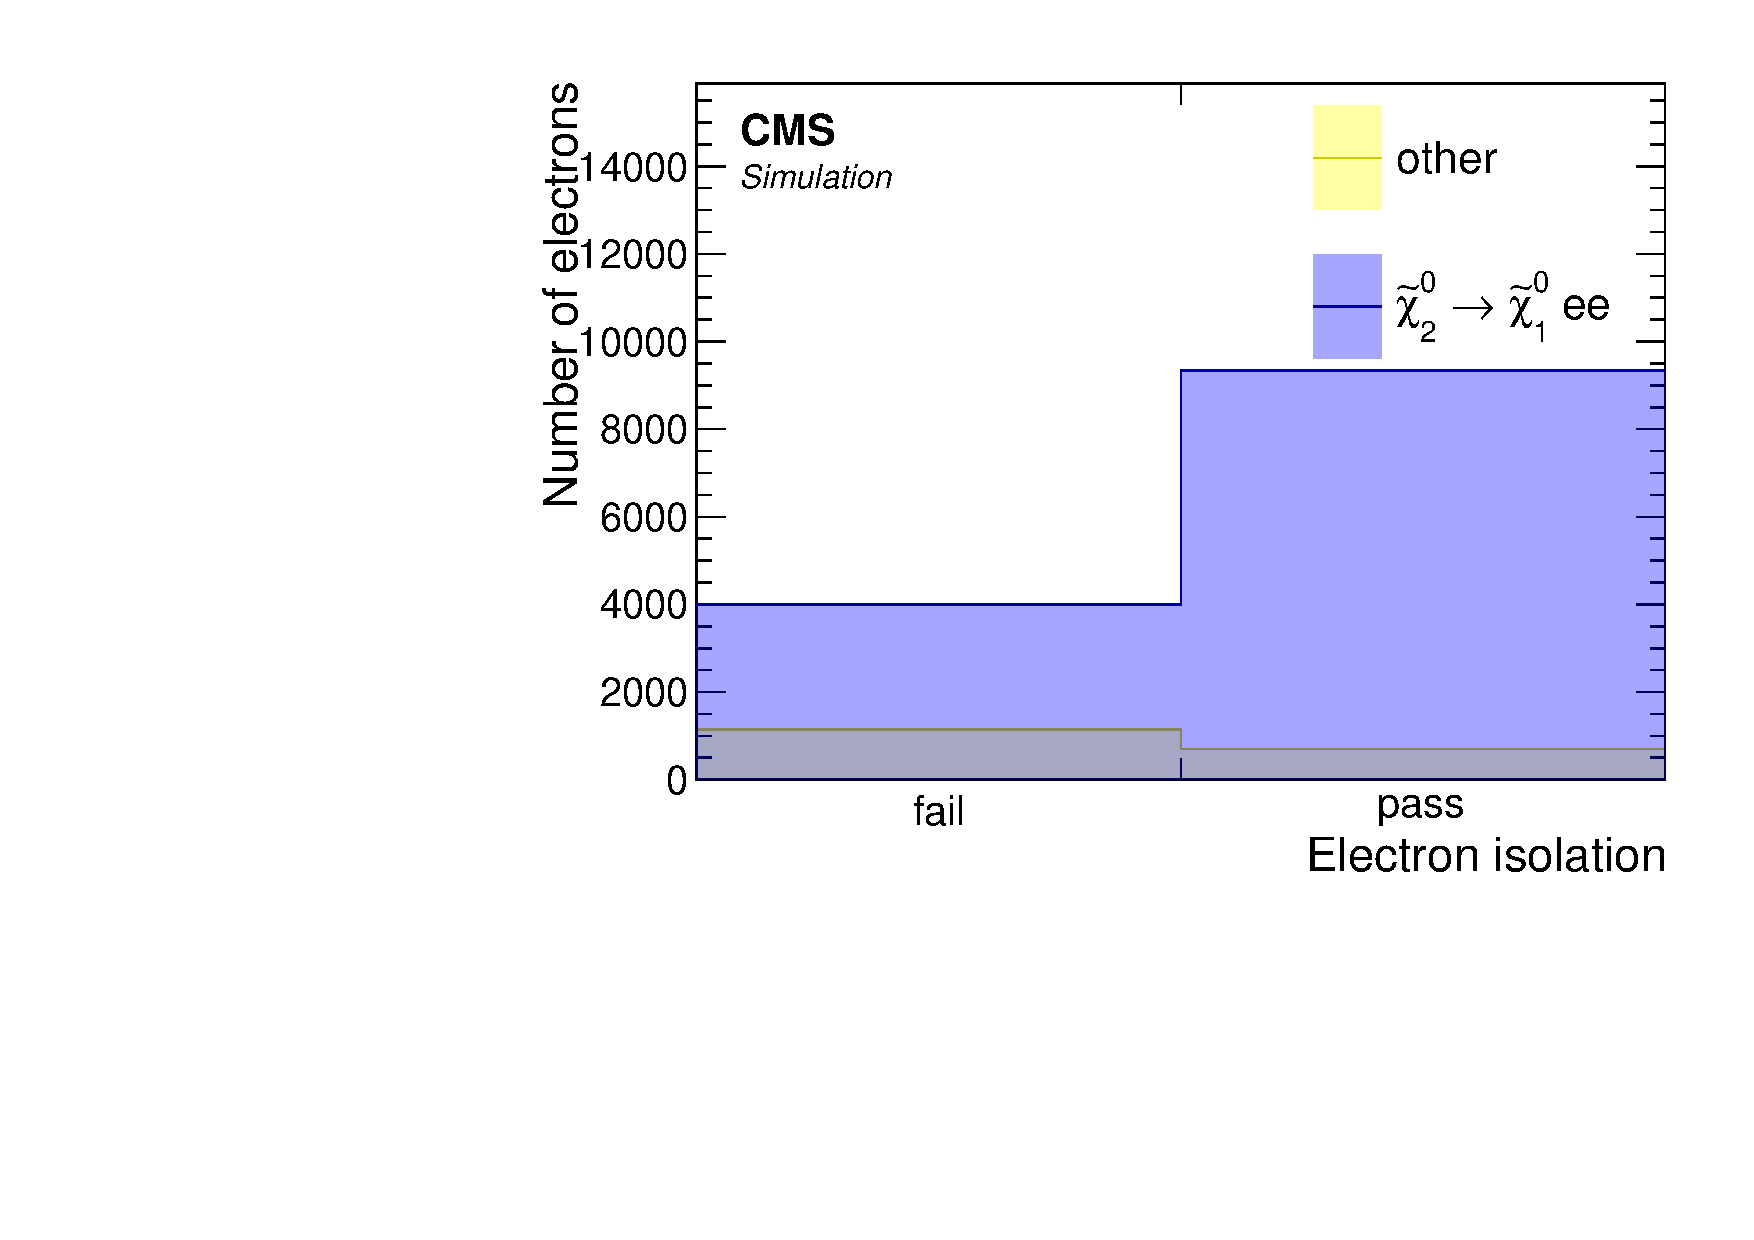
\includegraphics[width=0.48\linewidth]{plots/lepton_selection/lepton_selection_dm5p63/none_Electrons_iso.pdf} \,
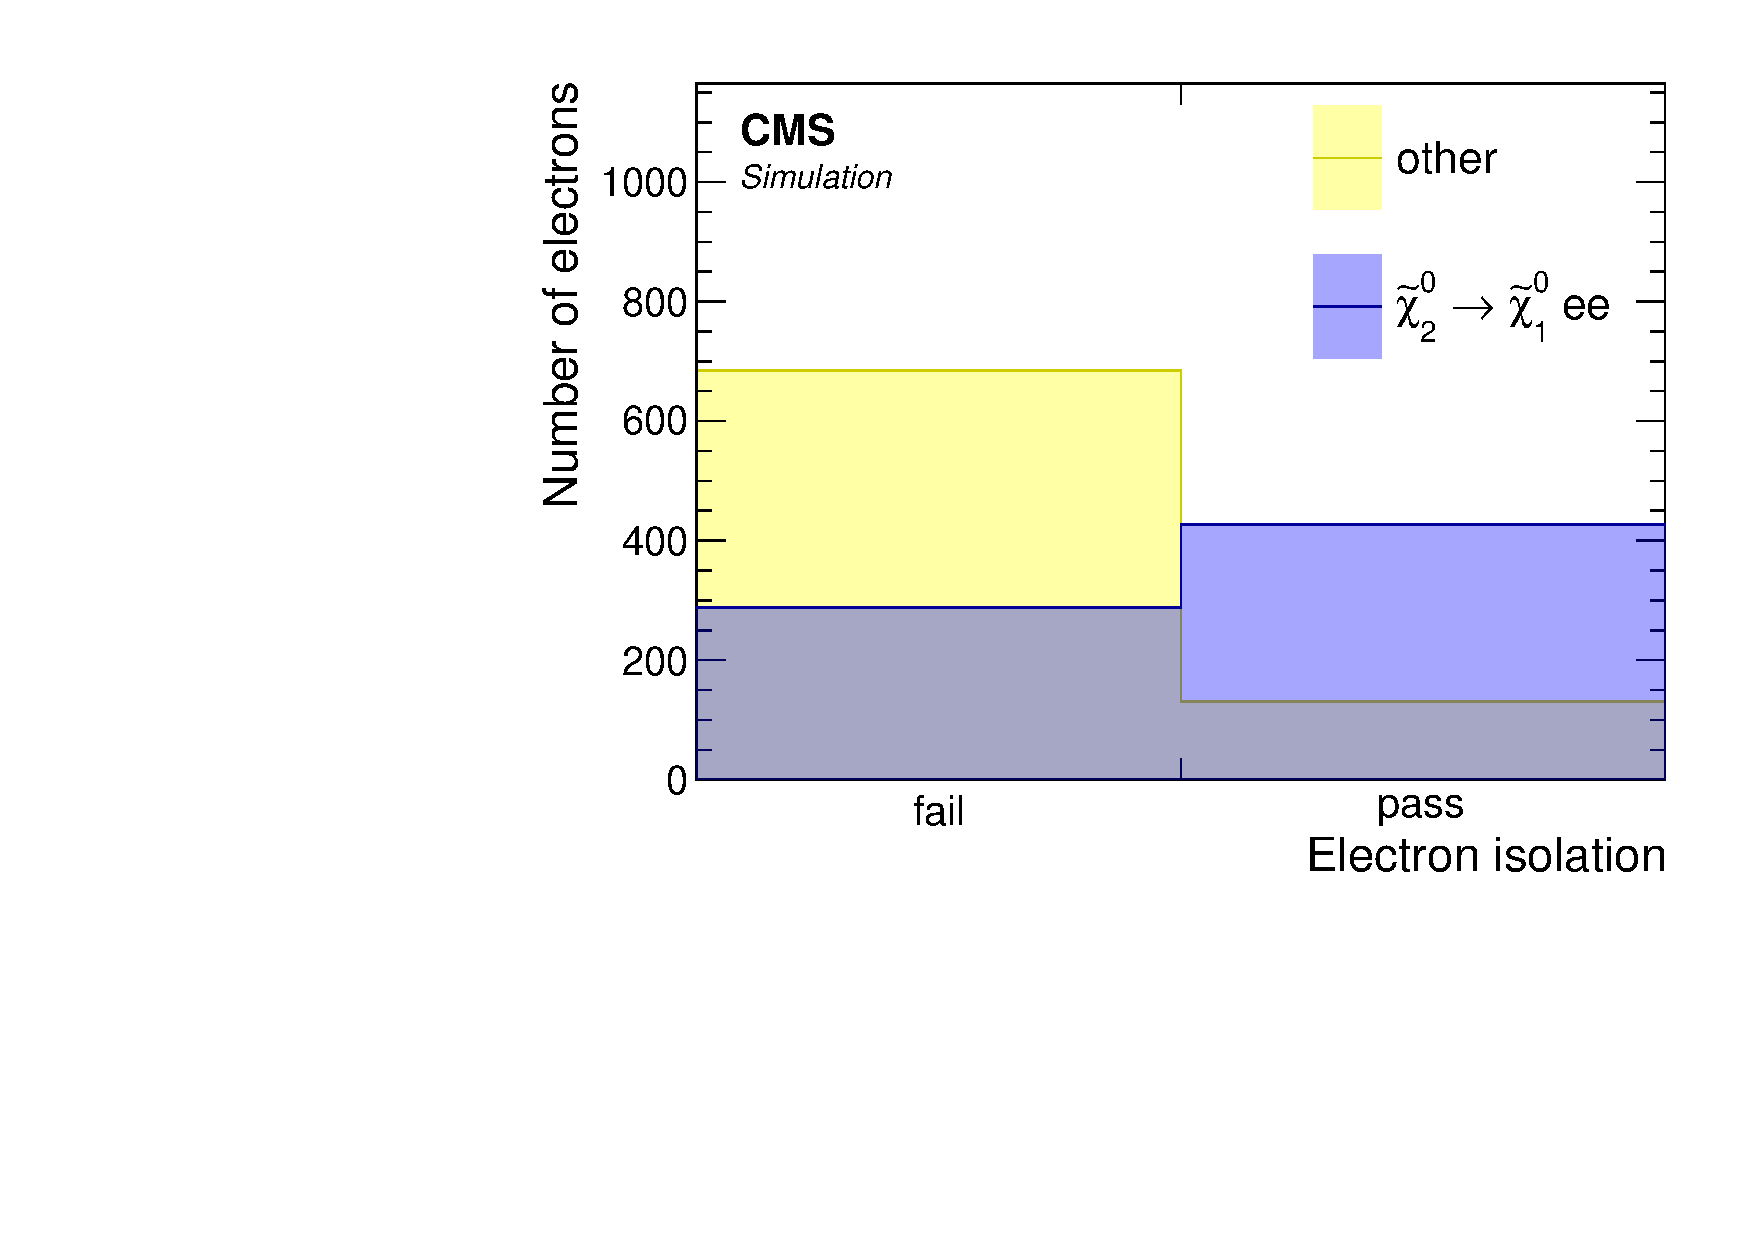
\includegraphics[width=0.48\linewidth]{plots/lepton_selection/lepton_selection_dm1p92/none_Electrons_iso.pdf}  \\
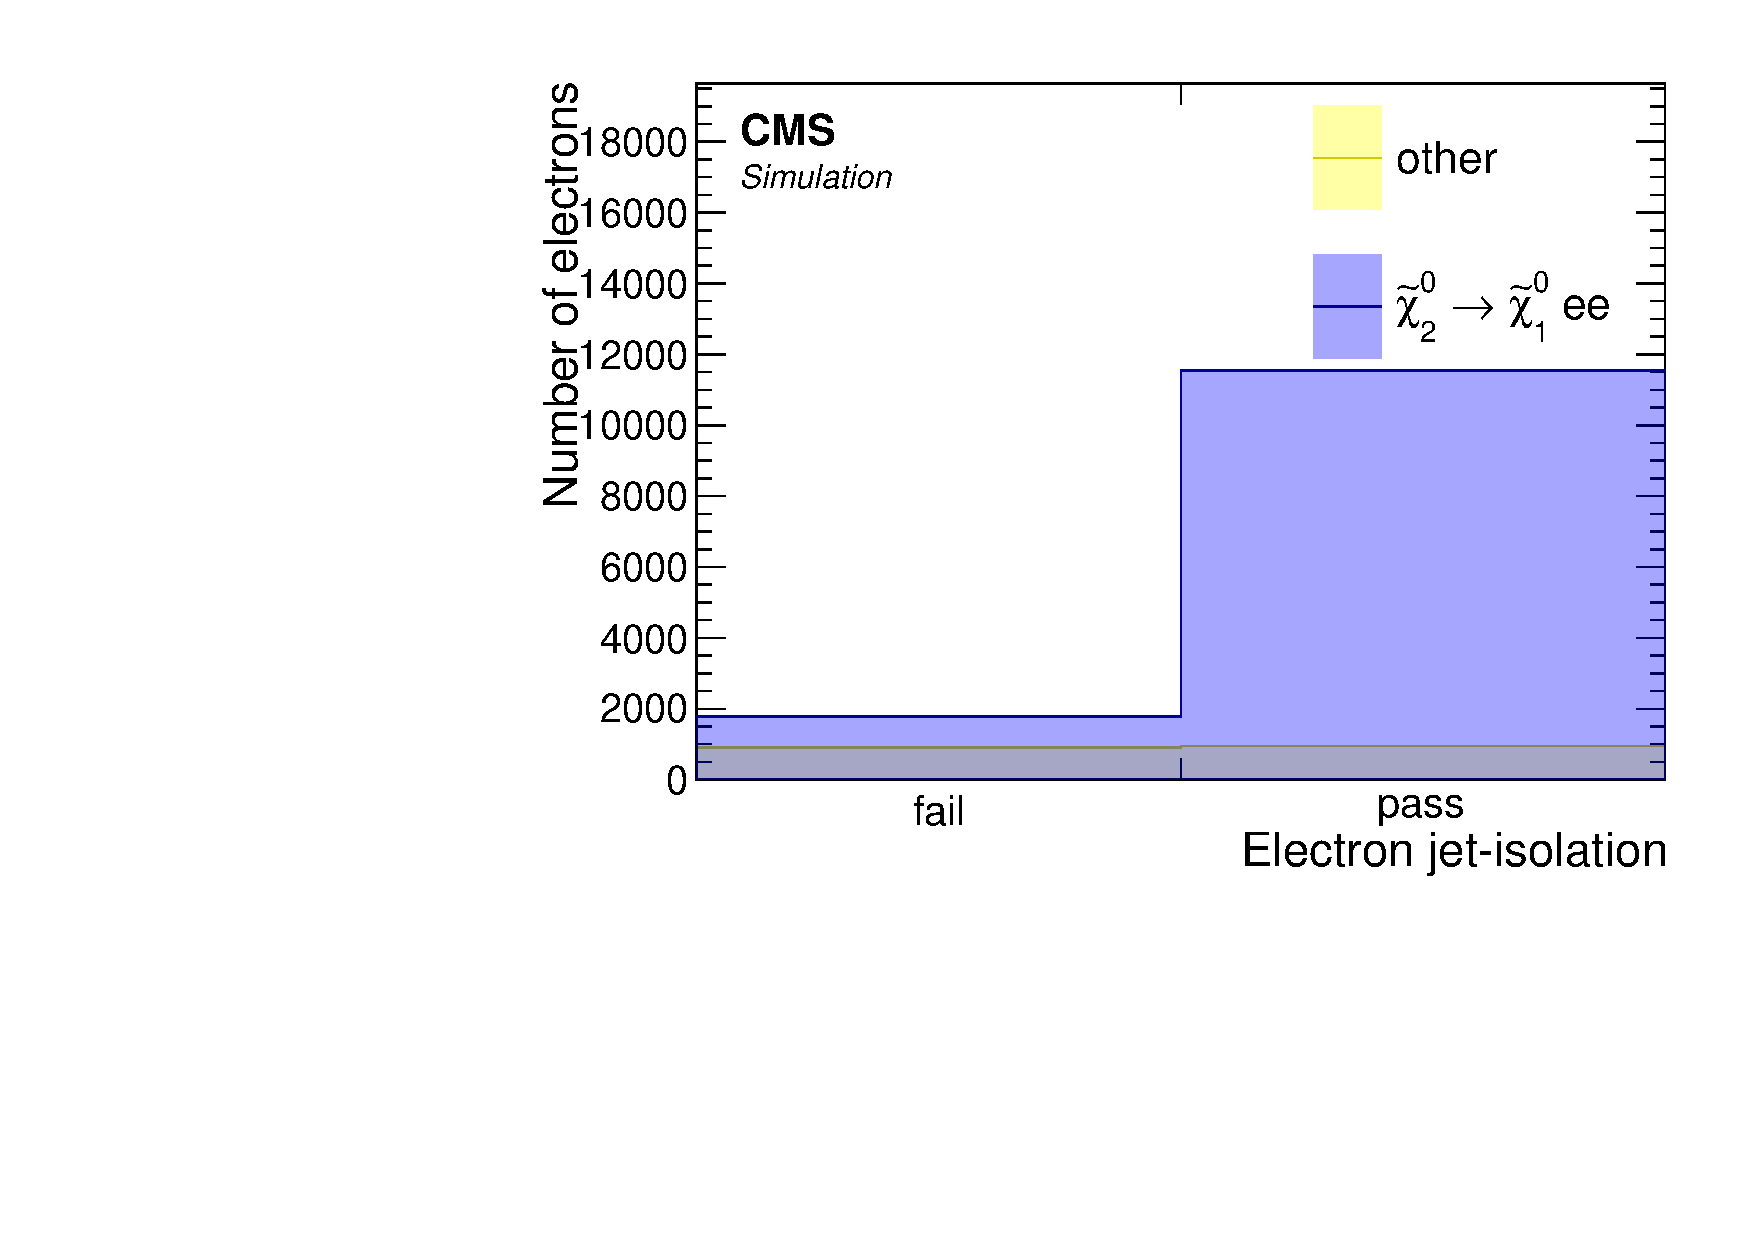
\includegraphics[width=0.48\linewidth]{plots/lepton_selection/lepton_selection_dm5p63/none_Electrons_CorrJetNoMultIso11Dr0.5.pdf} \,
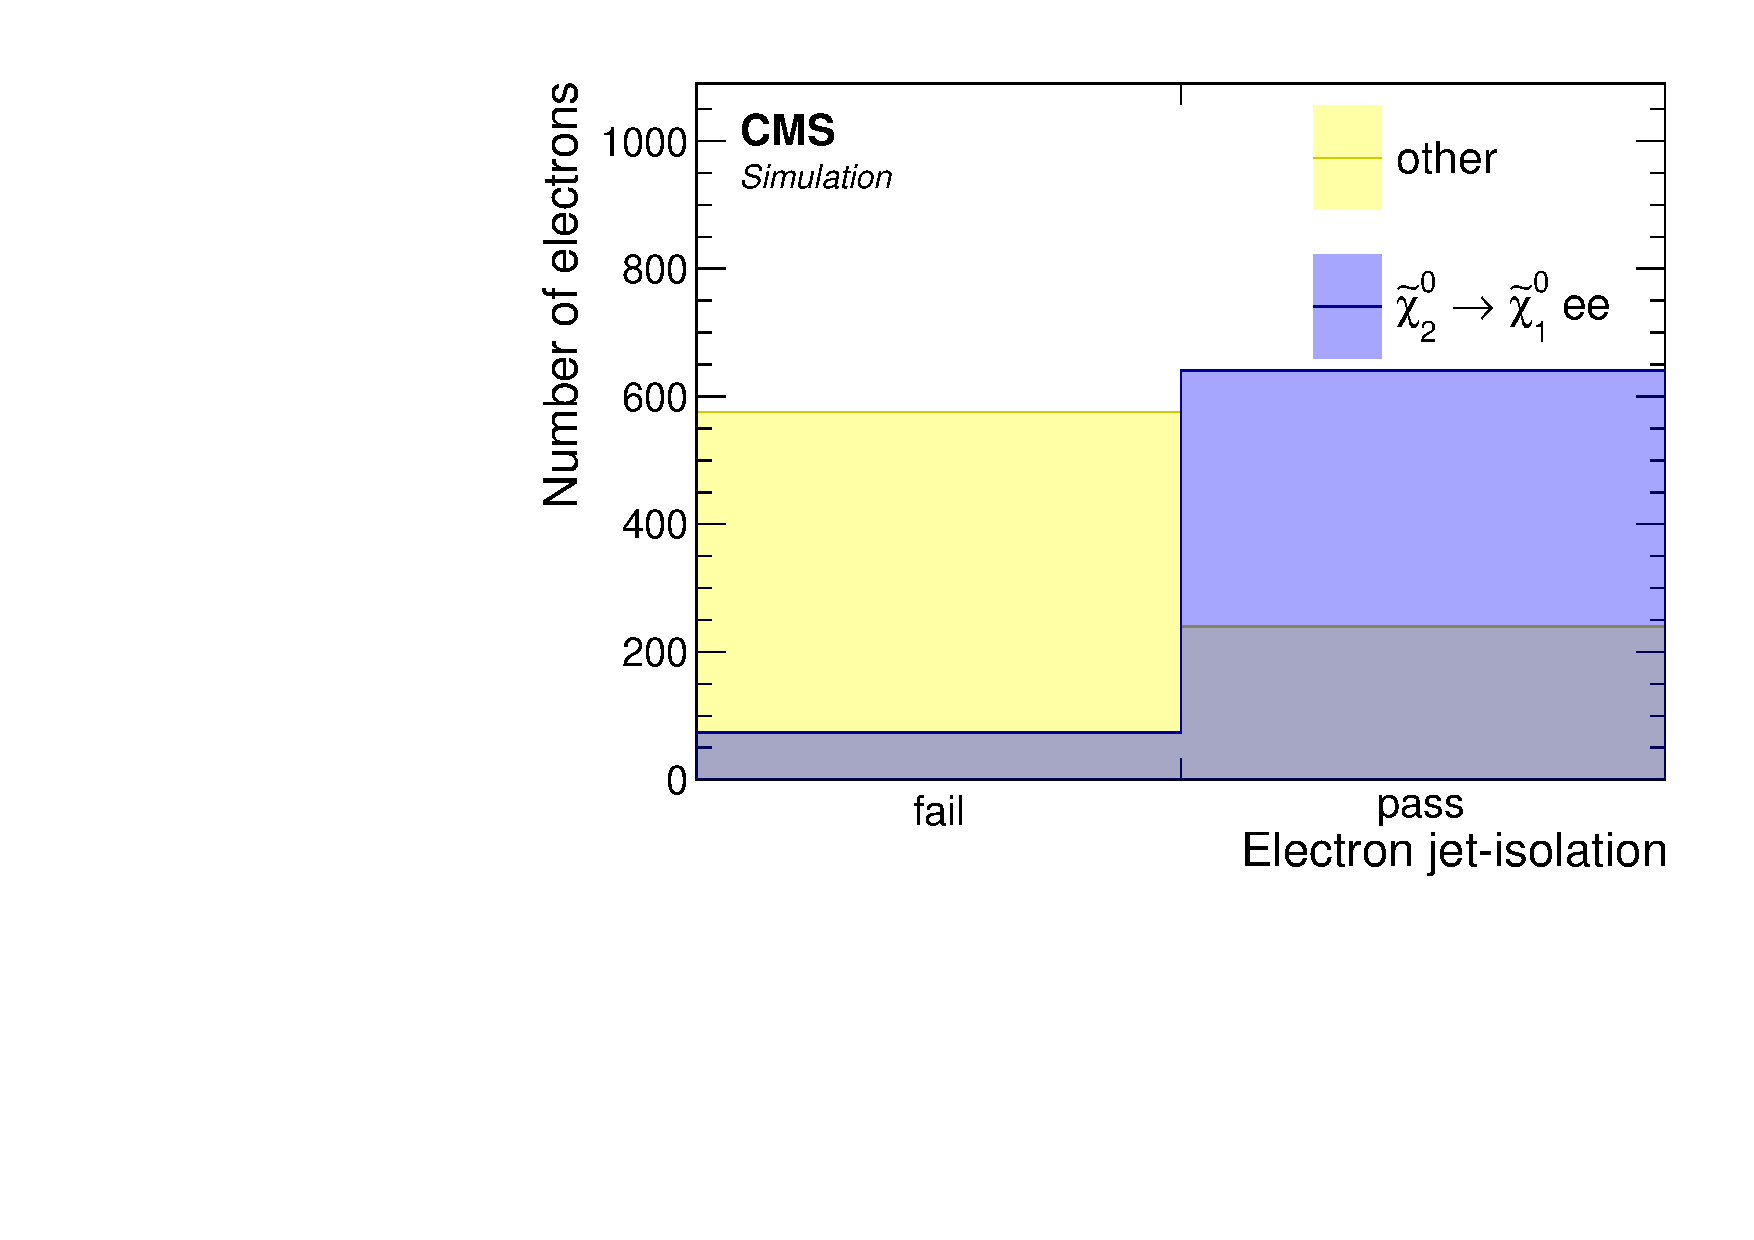
\includegraphics[width=0.48\linewidth]{plots/lepton_selection/lepton_selection_dm1p92/none_Electrons_CorrJetNoMultIso11Dr0.5.pdf}  \\
\caption[standard isolation and jet-isolation distribution of reconstructed electrons]{Standard isolation (top) and custom jet-isolation (bottom) distributions of reconstructed electrons with loose ID for $\dm=5.63\GeV$ (left) and $\dm=1.92\GeV$ (right). Cuts of $\DR(\jmath_1,\Pe)>0.4$ and $\pt<15\GeV$ are applied.}
\label{fig:electrons-selection-isolation}
\end{figure}

We observe that the standard lepton isolation does not perform well in terms of efficiency for both \dm cases. In contrast, the custom jet-isolation is performing very well in terms of signal electron efficiency while successfully rejecting considerable amount of non-signal electrons, resulting in a purer sample of electrons.

\subsubsection{Additional electron veto}
\subsubsection{Selection summary}
\subsection{Muons}
\subsubsection{Signal muon selection}
\label{sec:muon-selection}
\subsubsection{Additional muon veto}

\subsection{Missing transverse energy}
\label{subsec:met}

\subsection{Scale factors}

\begin{figure}[]
\centering
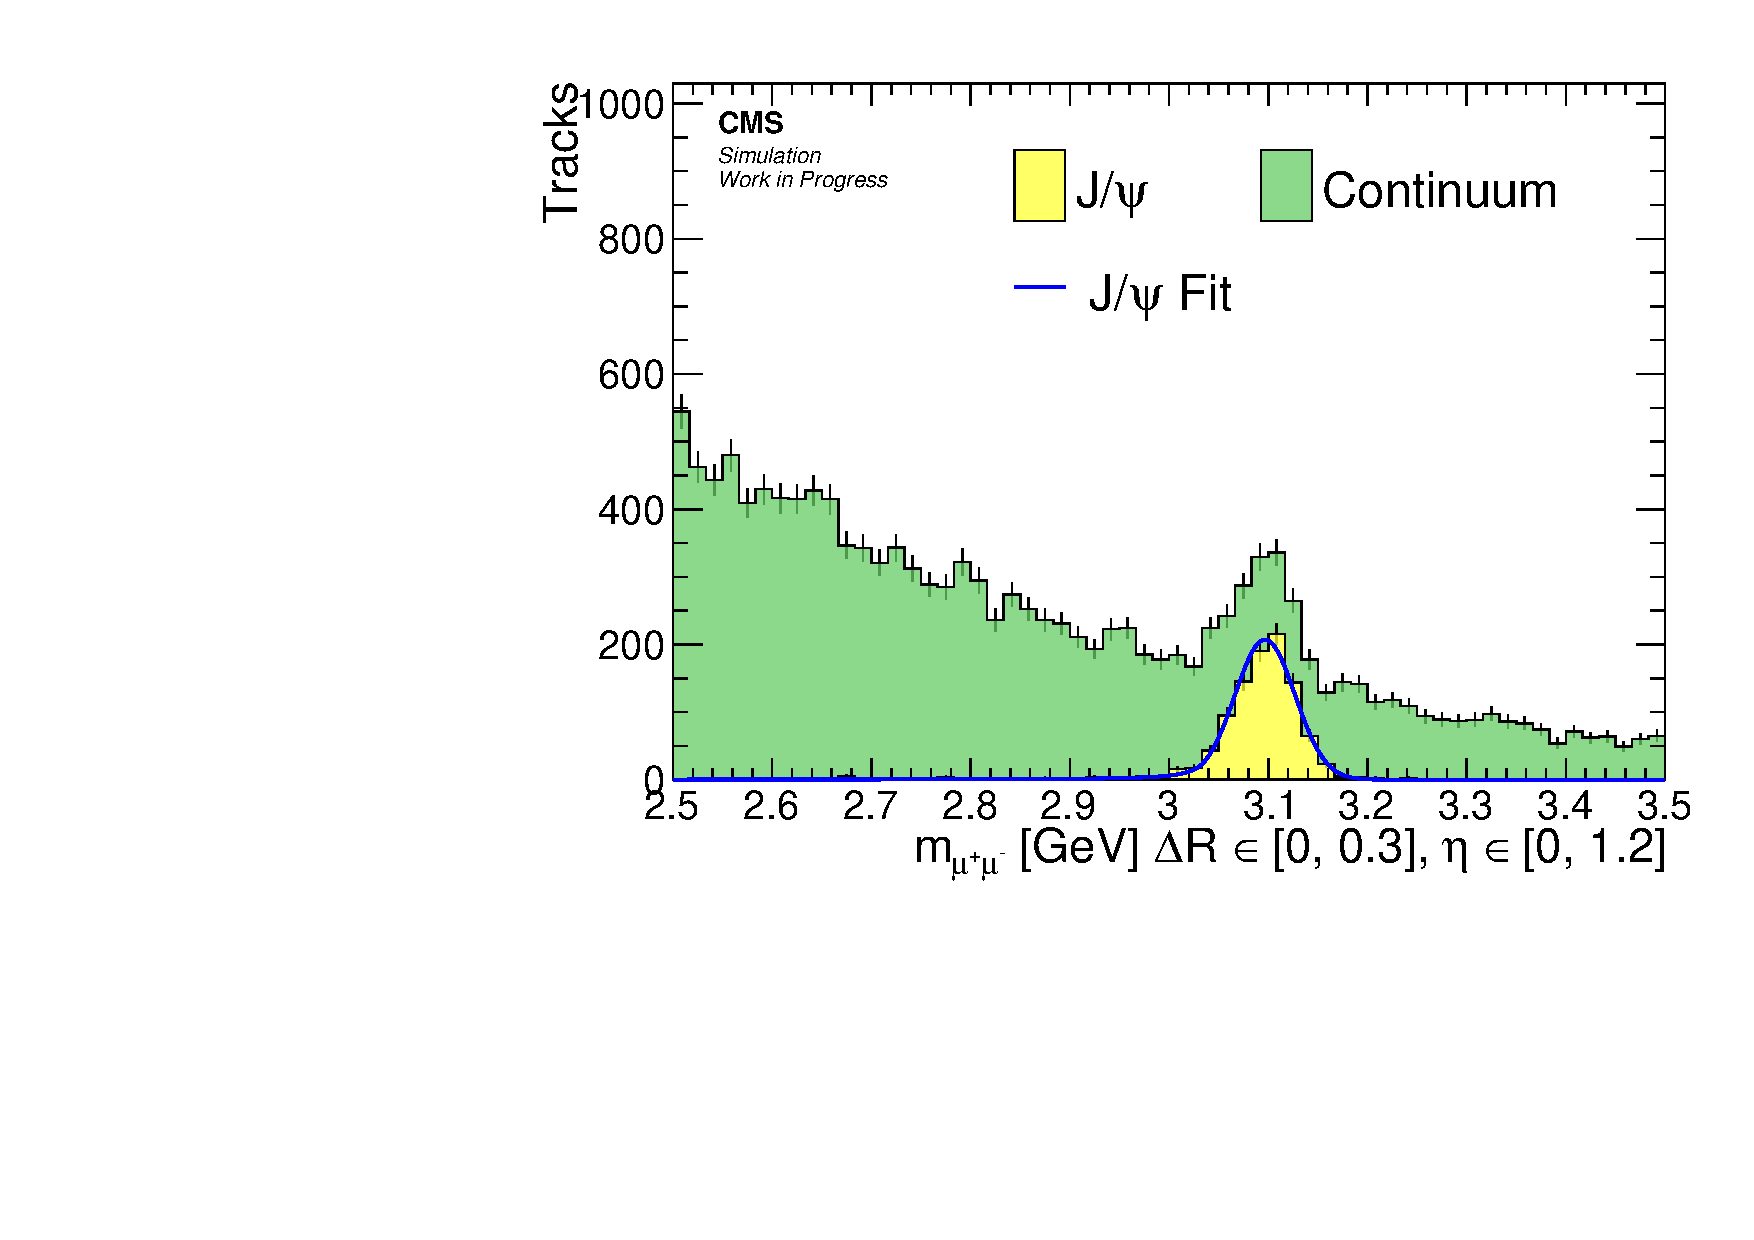
\includegraphics[width=0.32\linewidth]{plots/jpsi_muons_fit_bg_delta_r_single_electron/none_invMass_0_0.3_0_1.2.pdf} \,
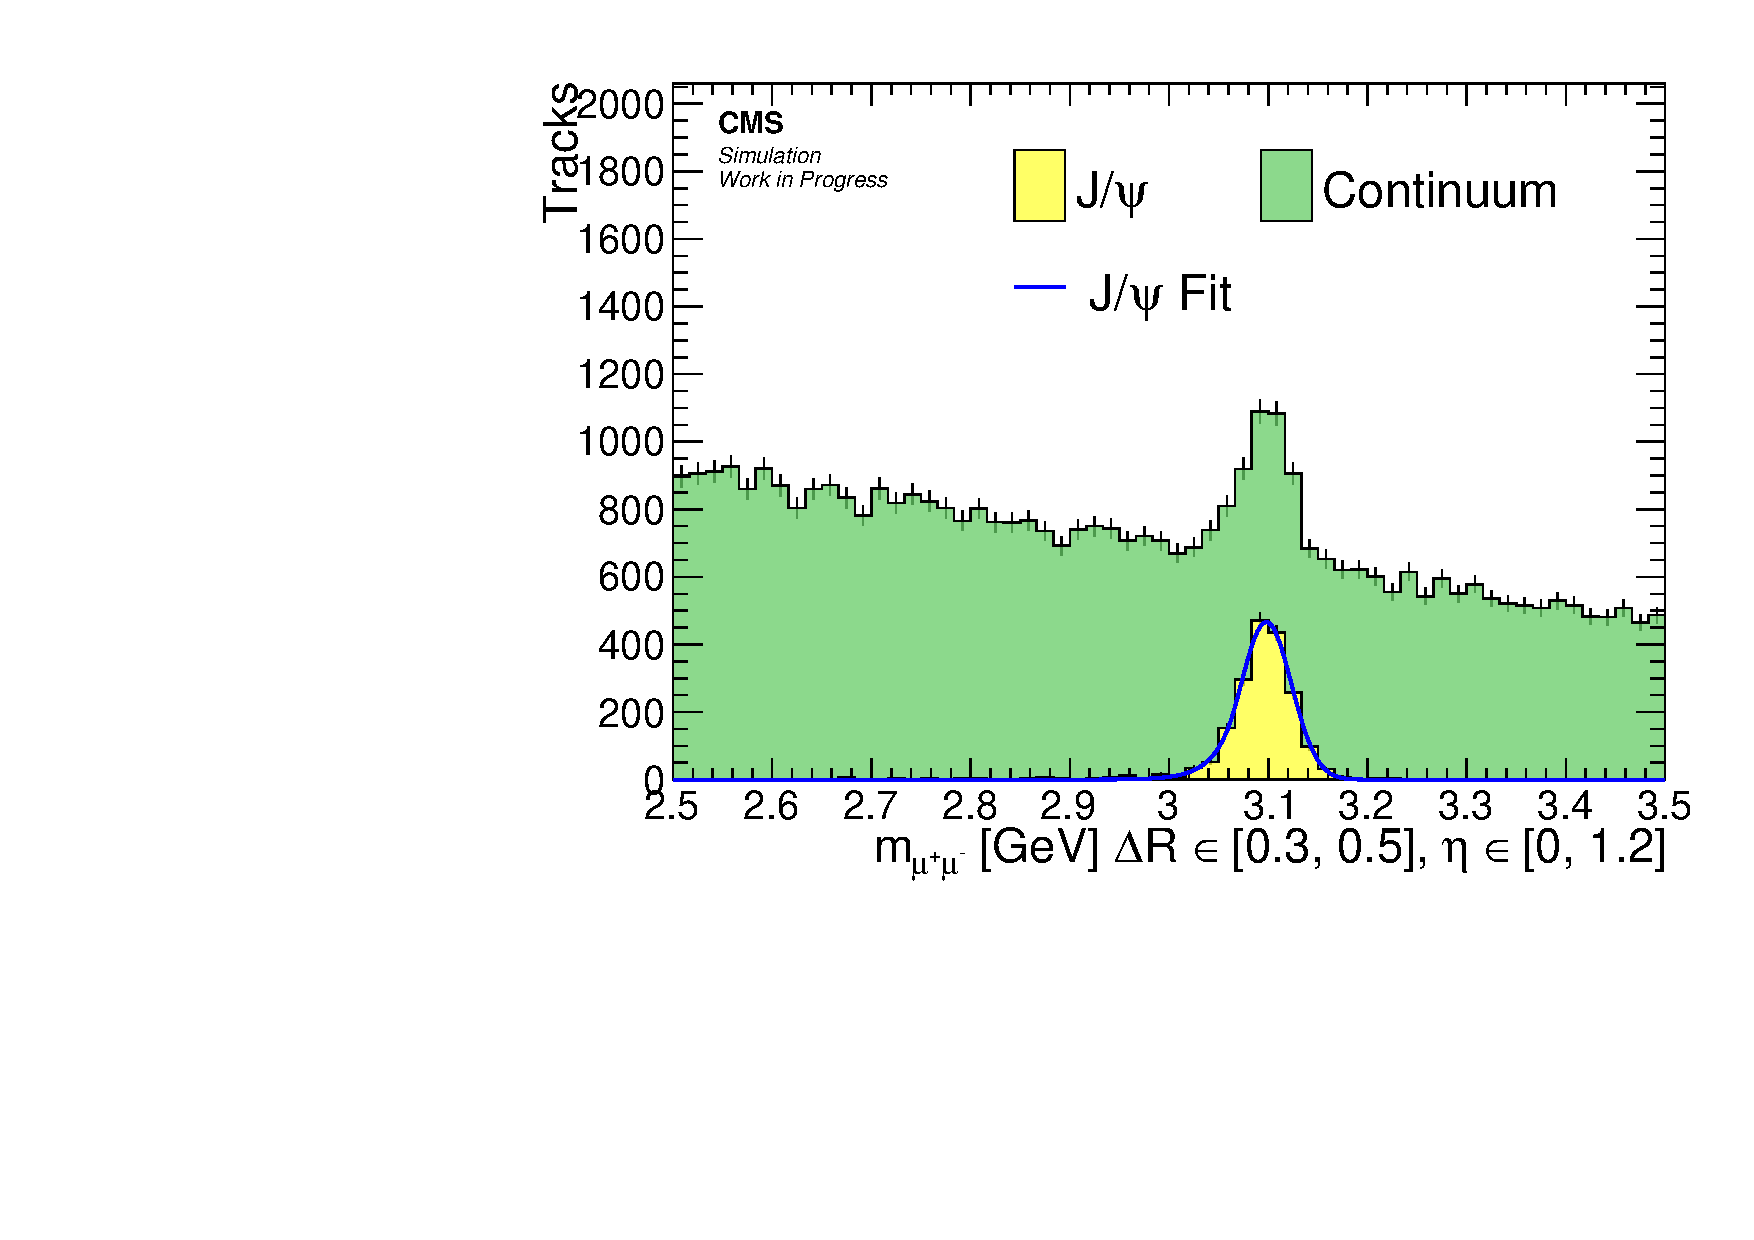
\includegraphics[width=0.32\linewidth]{plots/jpsi_muons_fit_bg_delta_r_single_electron/none_invMass_0.3_0.5_0_1.2.pdf}  \,
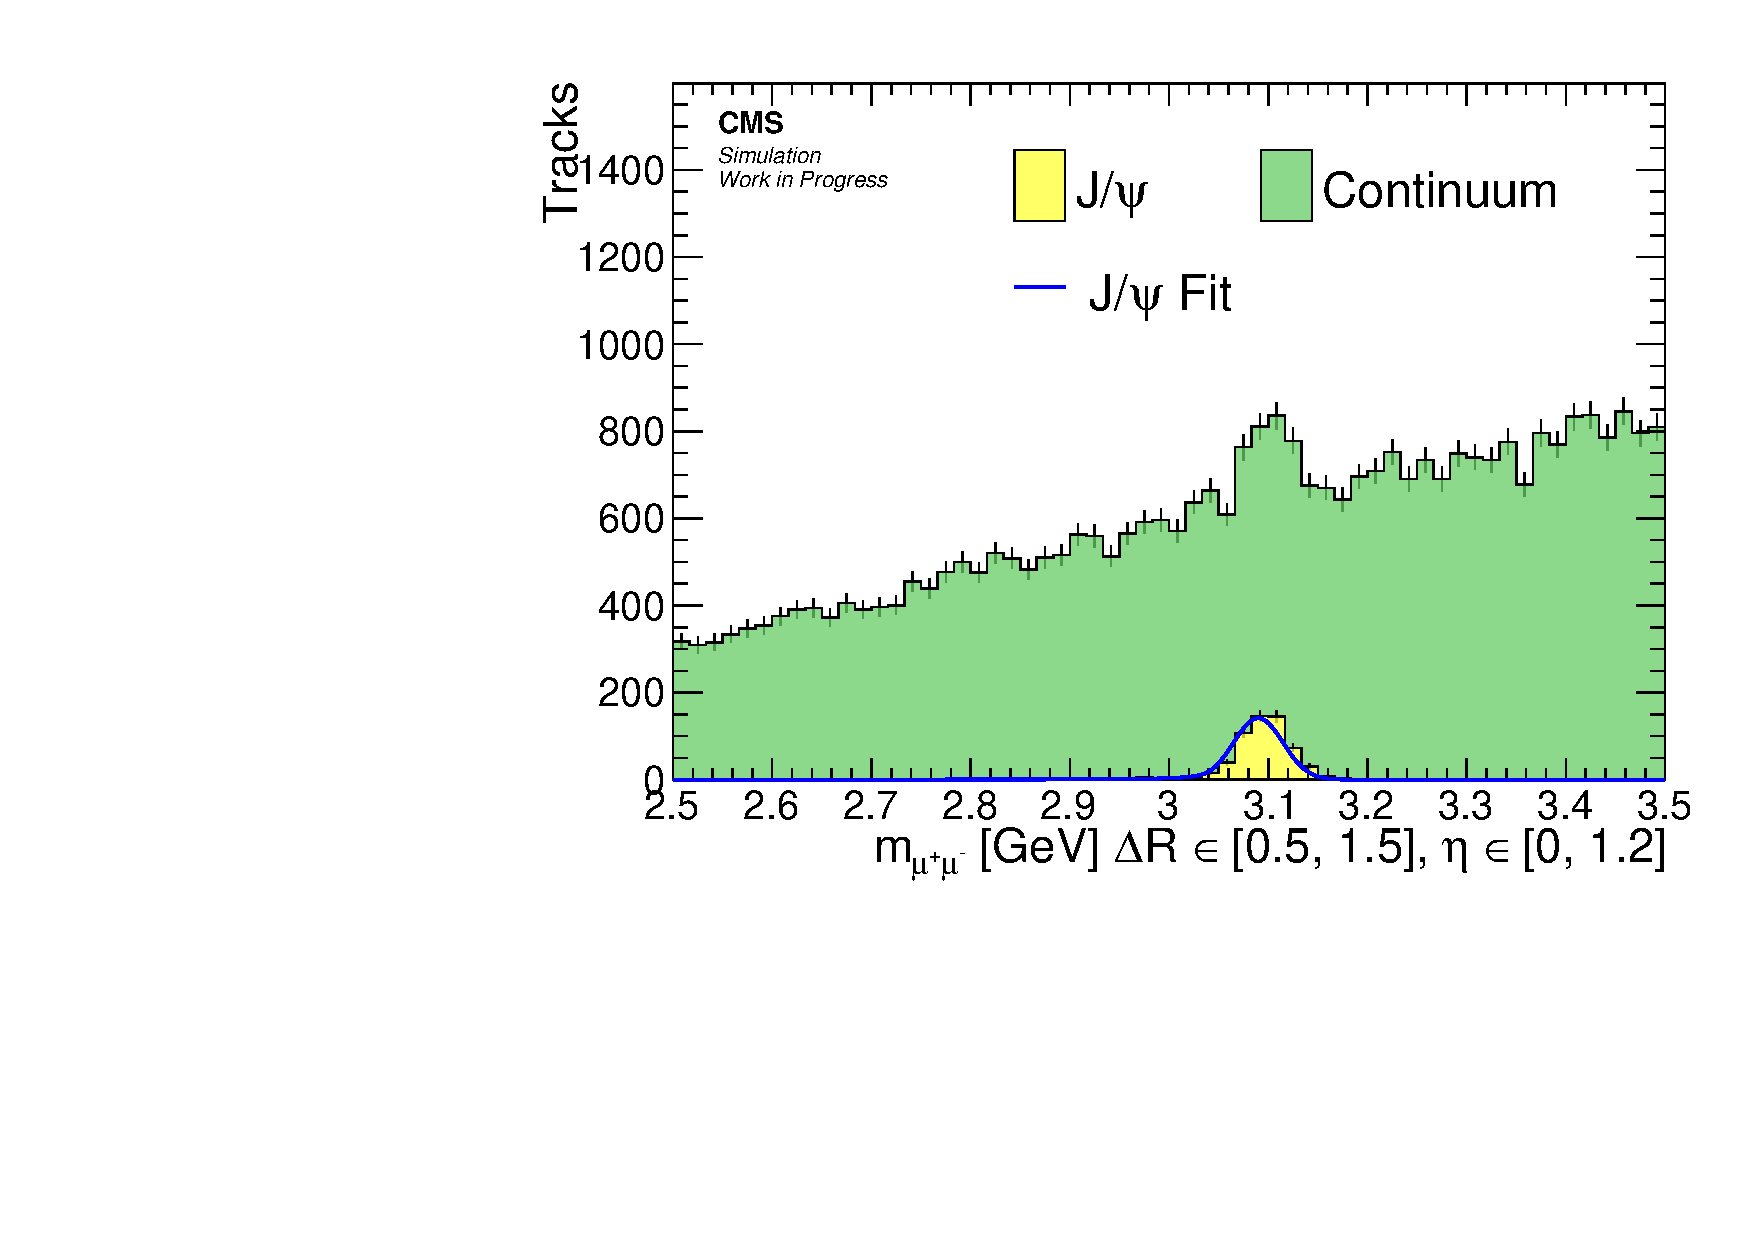
\includegraphics[width=0.32\linewidth]{plots/jpsi_muons_fit_bg_delta_r_single_electron/none_invMass_0.5_1.5_0_1.2.pdf} \\
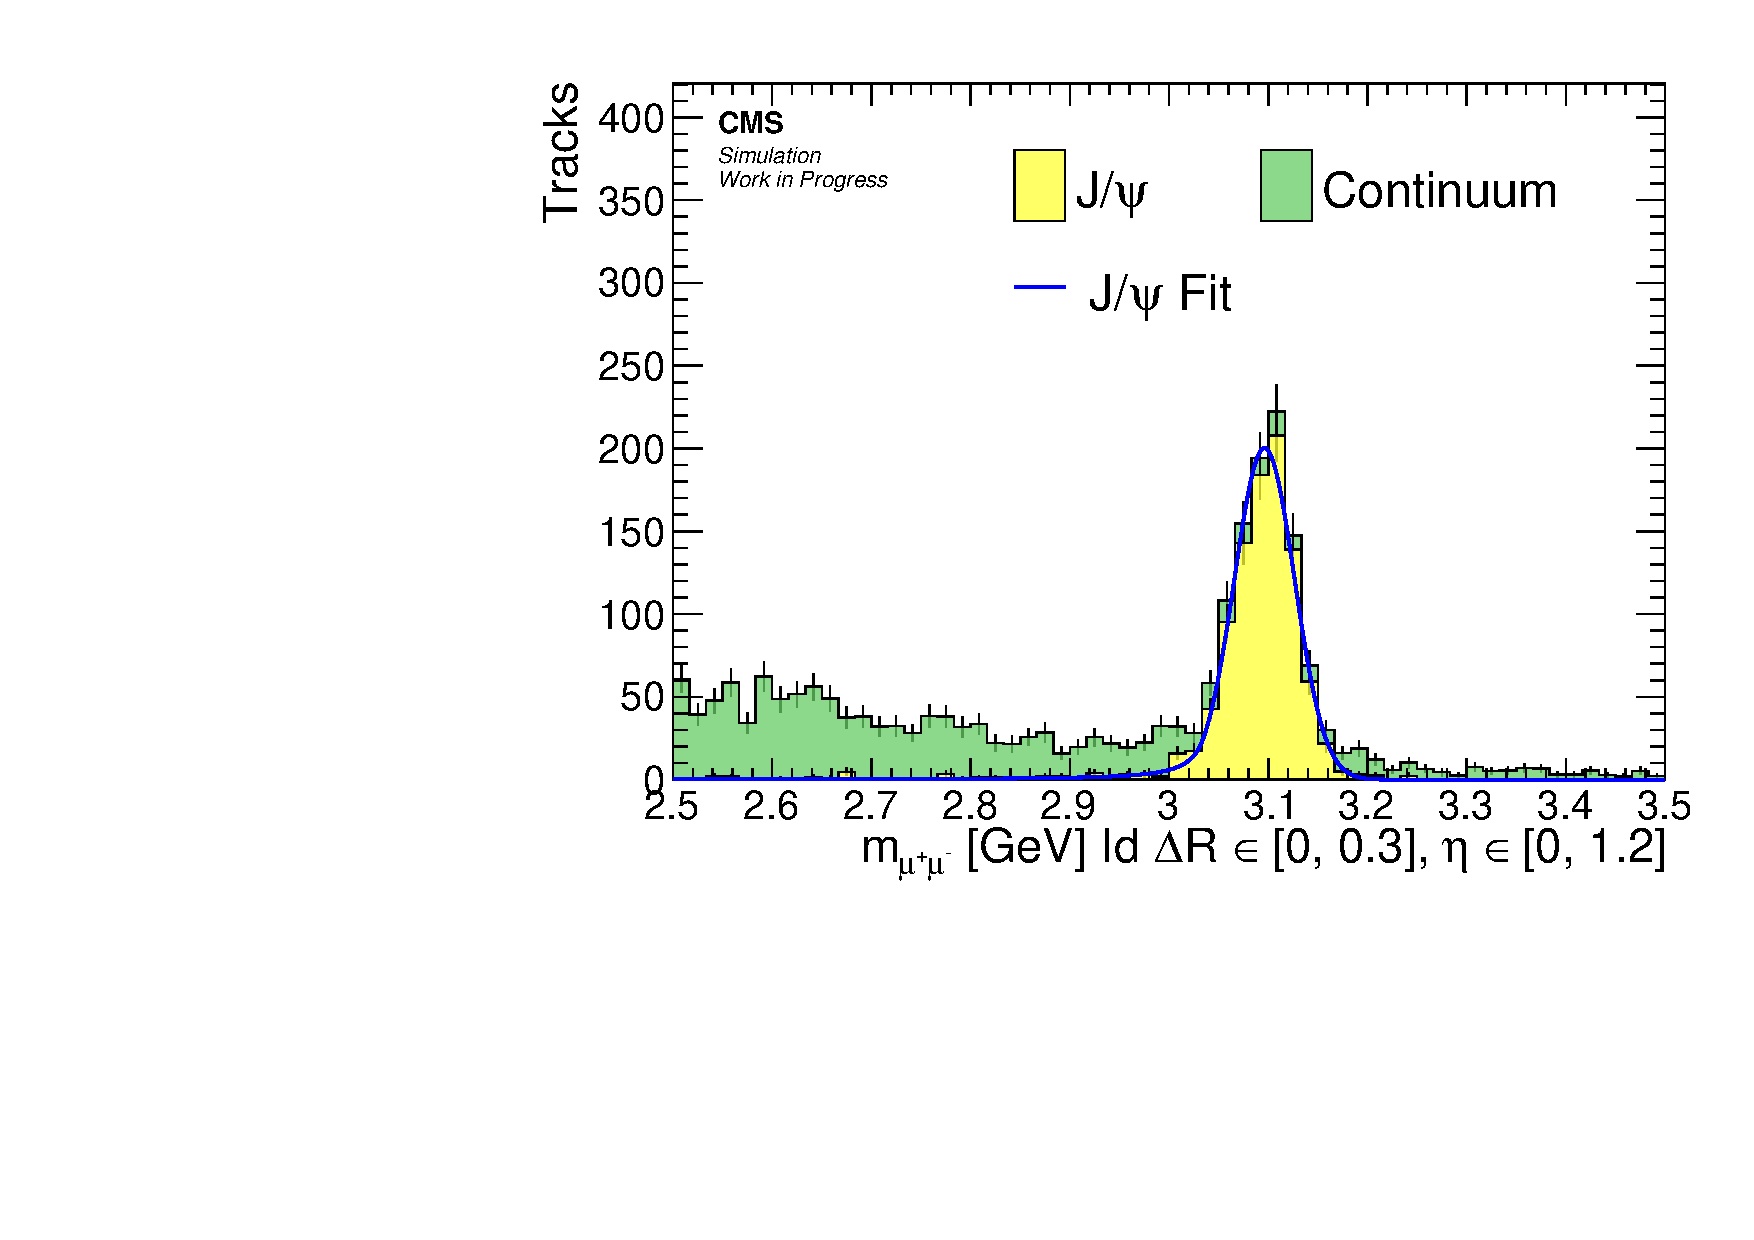
\includegraphics[width=0.32\linewidth]{plots/jpsi_muons_fit_bg_delta_r_single_electron/none_id_invMass_0_0.3_0_1.2.pdf} \,
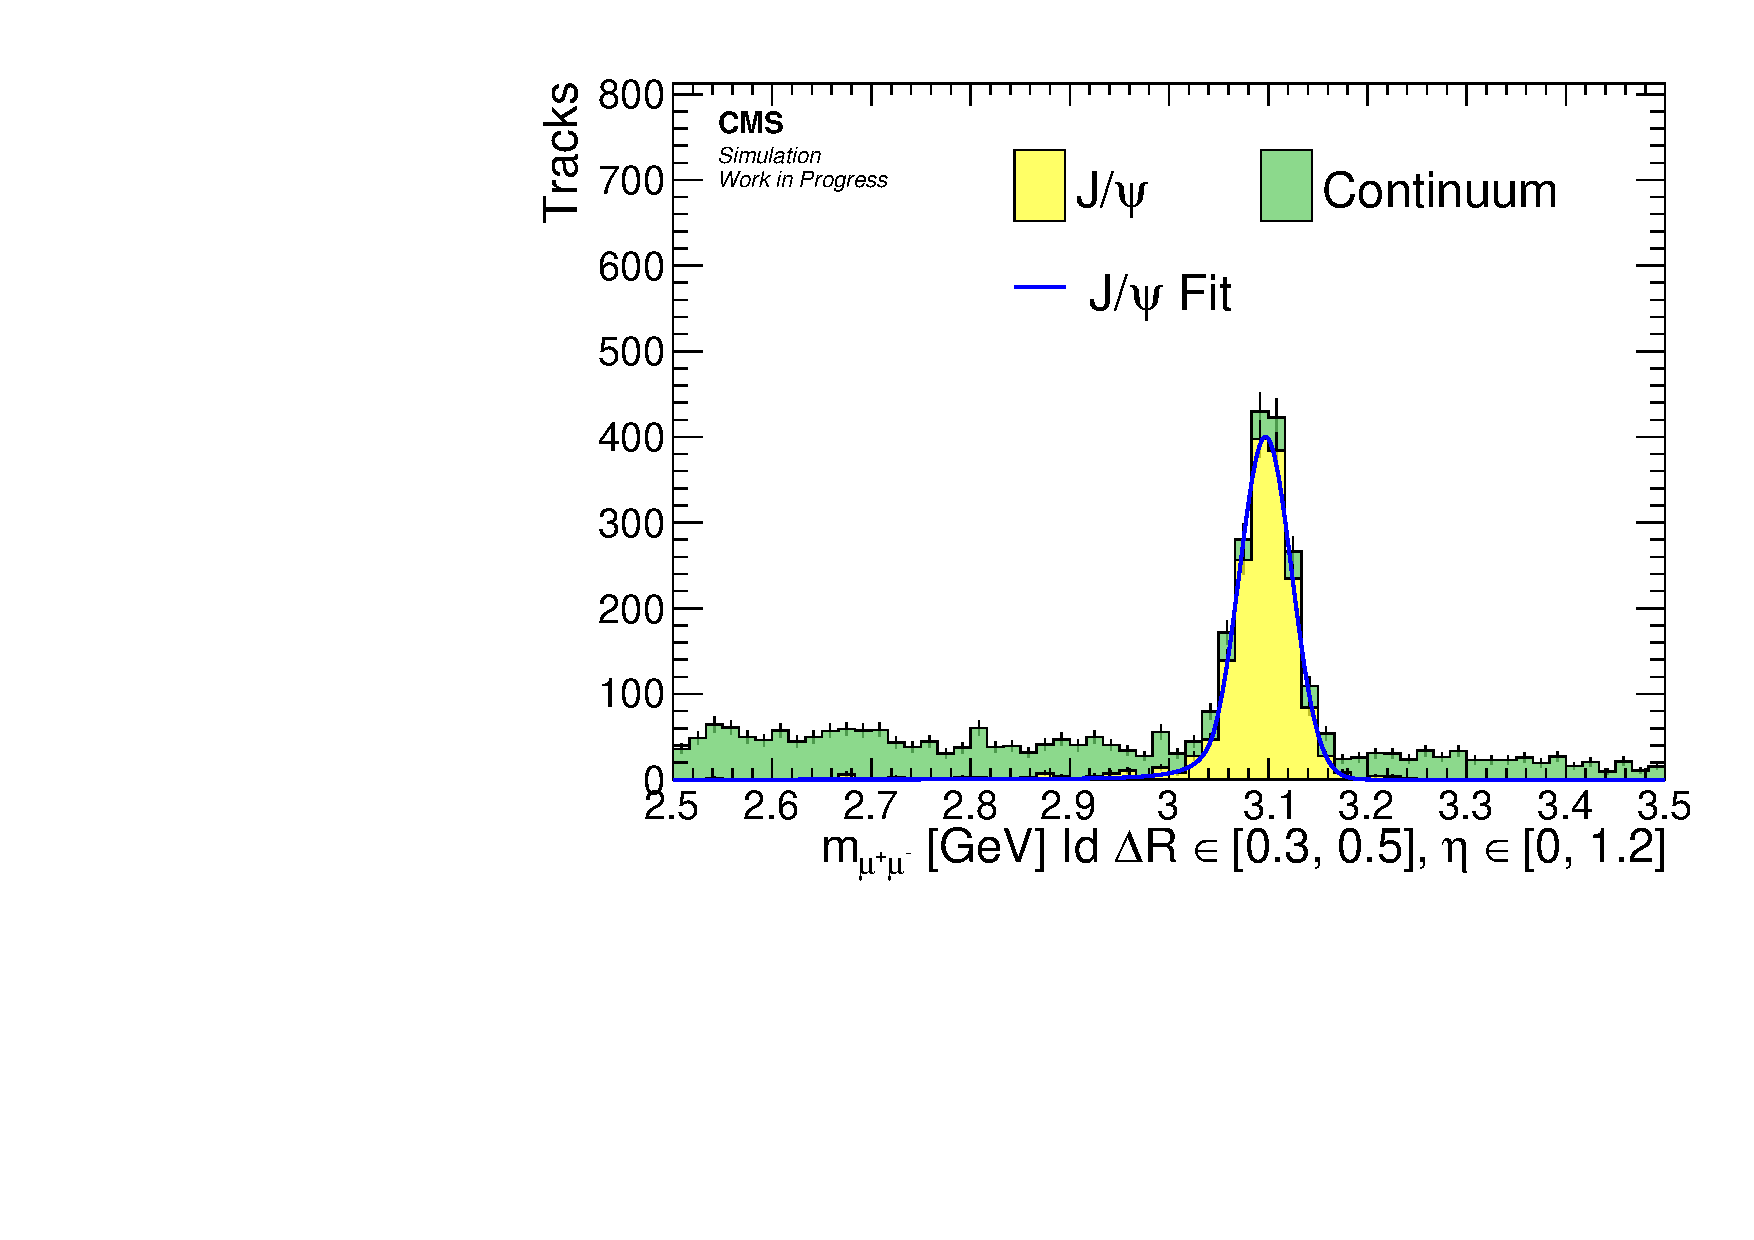
\includegraphics[width=0.32\linewidth]{plots/jpsi_muons_fit_bg_delta_r_single_electron/none_id_invMass_0.3_0.5_0_1.2.pdf}  \,
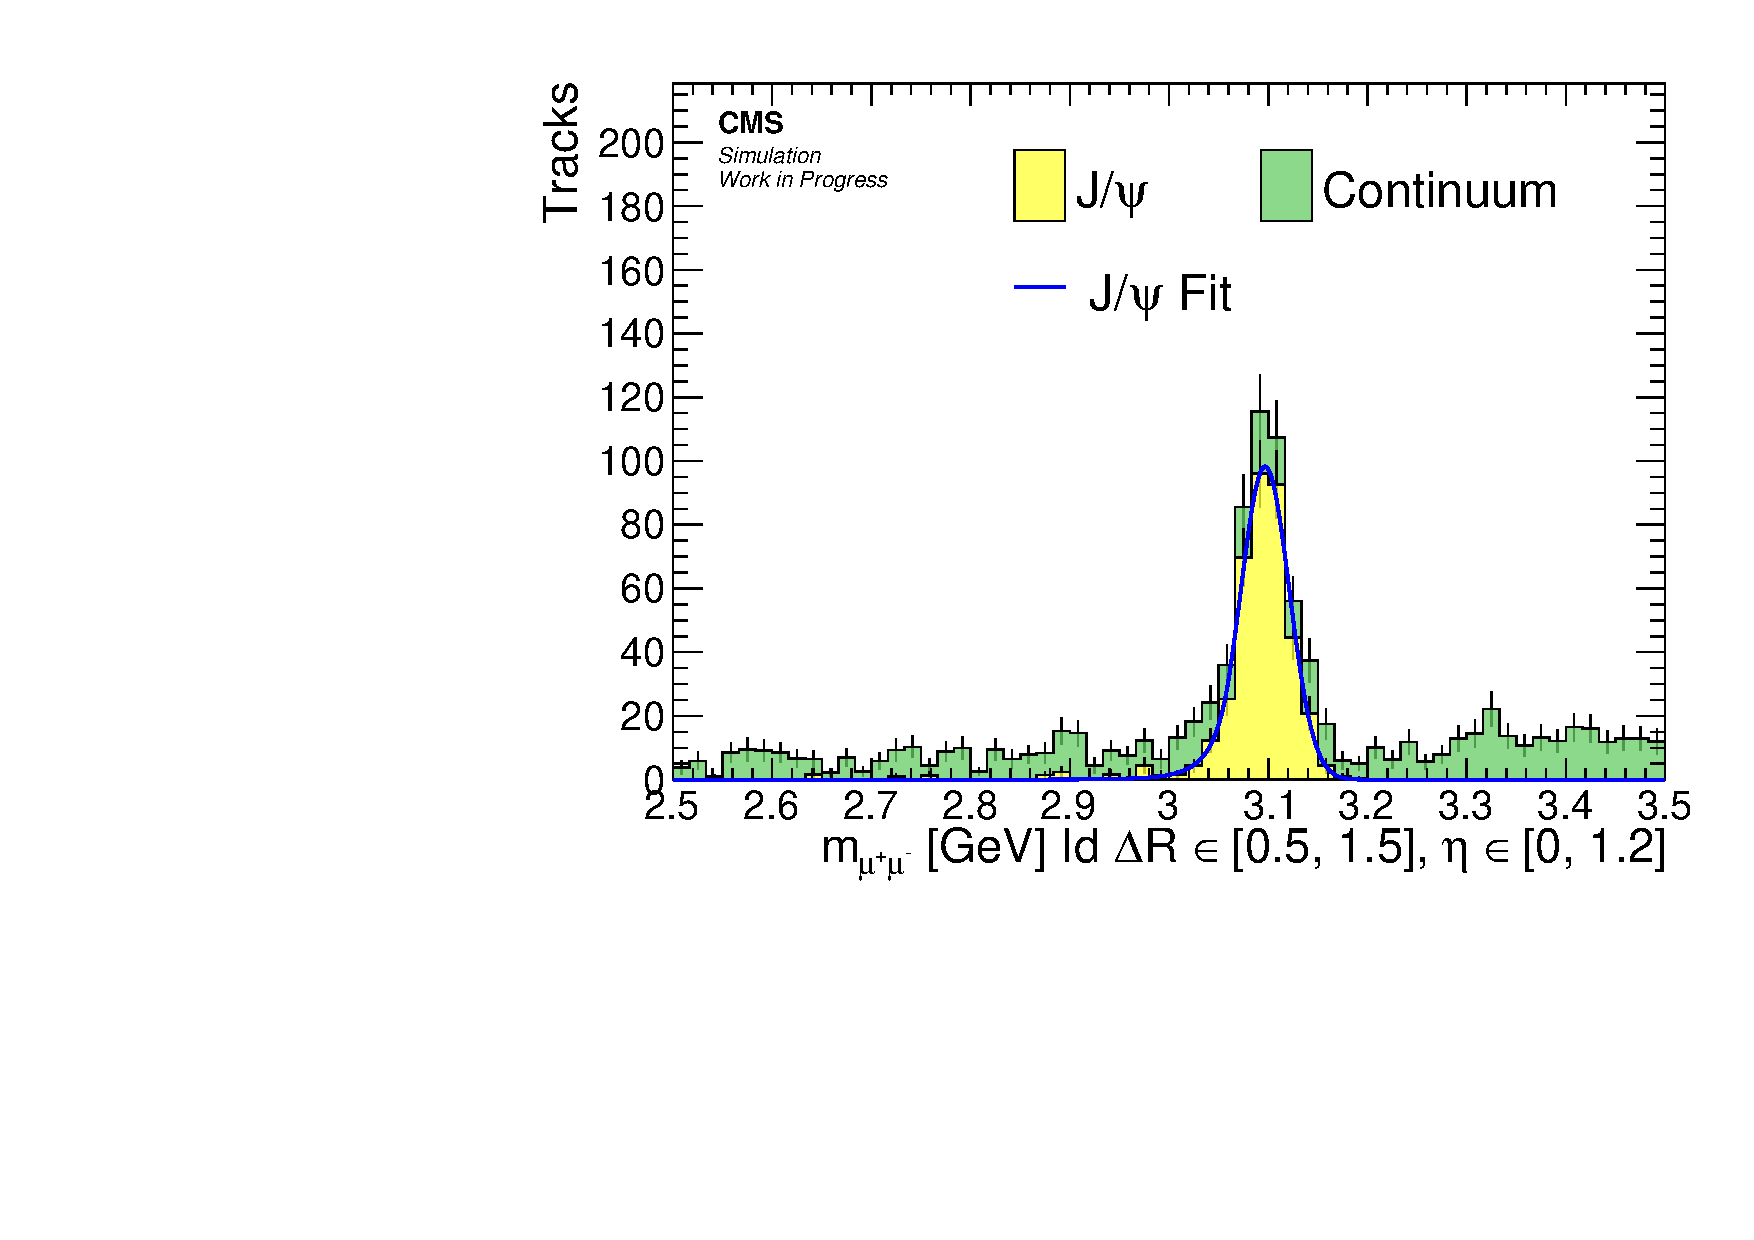
\includegraphics[width=0.32\linewidth]{plots/jpsi_muons_fit_bg_delta_r_single_electron/none_id_invMass_0.5_1.5_0_1.2.pdf} \\
\caption[Barrel BG]{Barrel Muons BG}
\label{fig:tb-barrel-simulation}
\end{figure}

\begin{figure}[]
\centering
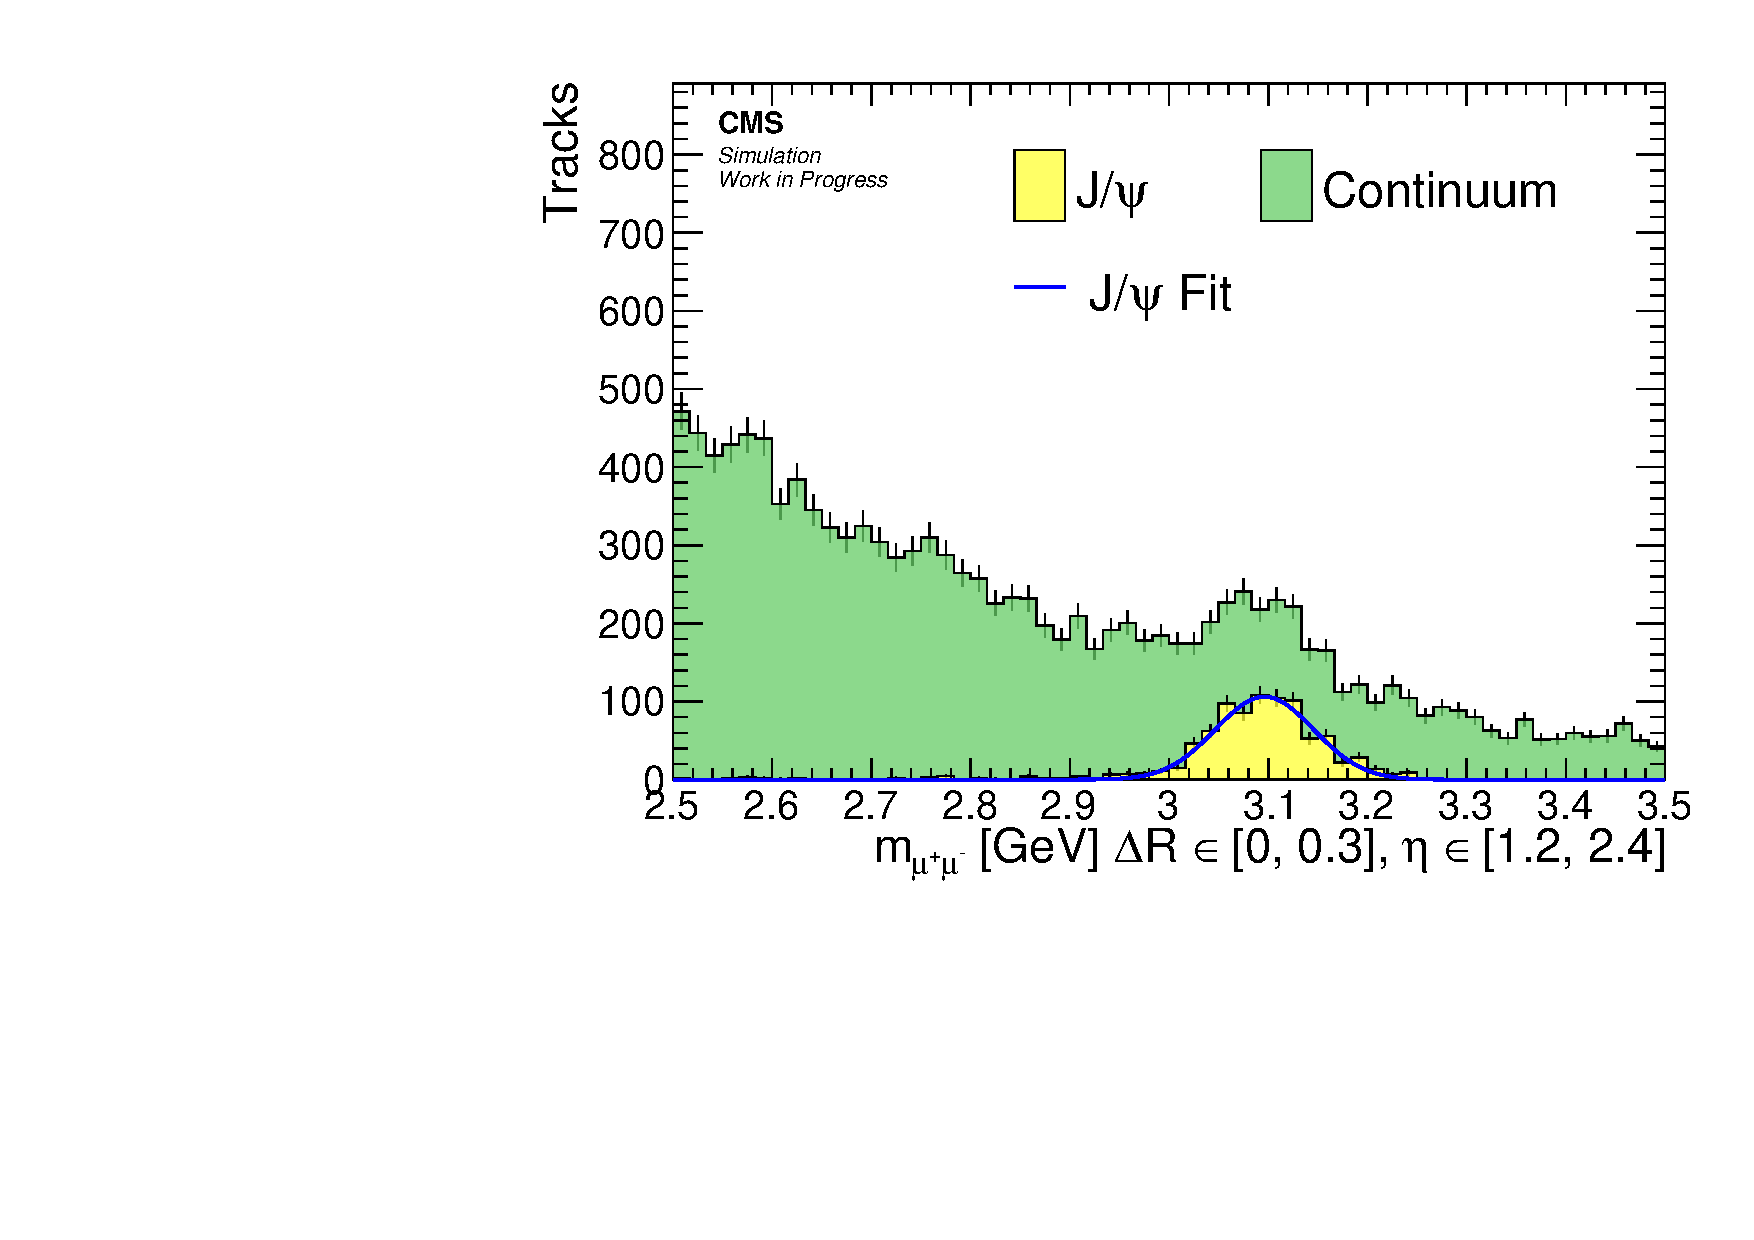
\includegraphics[width=0.32\linewidth]{plots/jpsi_muons_fit_bg_delta_r_single_electron/none_invMass_0_0.3_1.2_2.4.pdf} \,
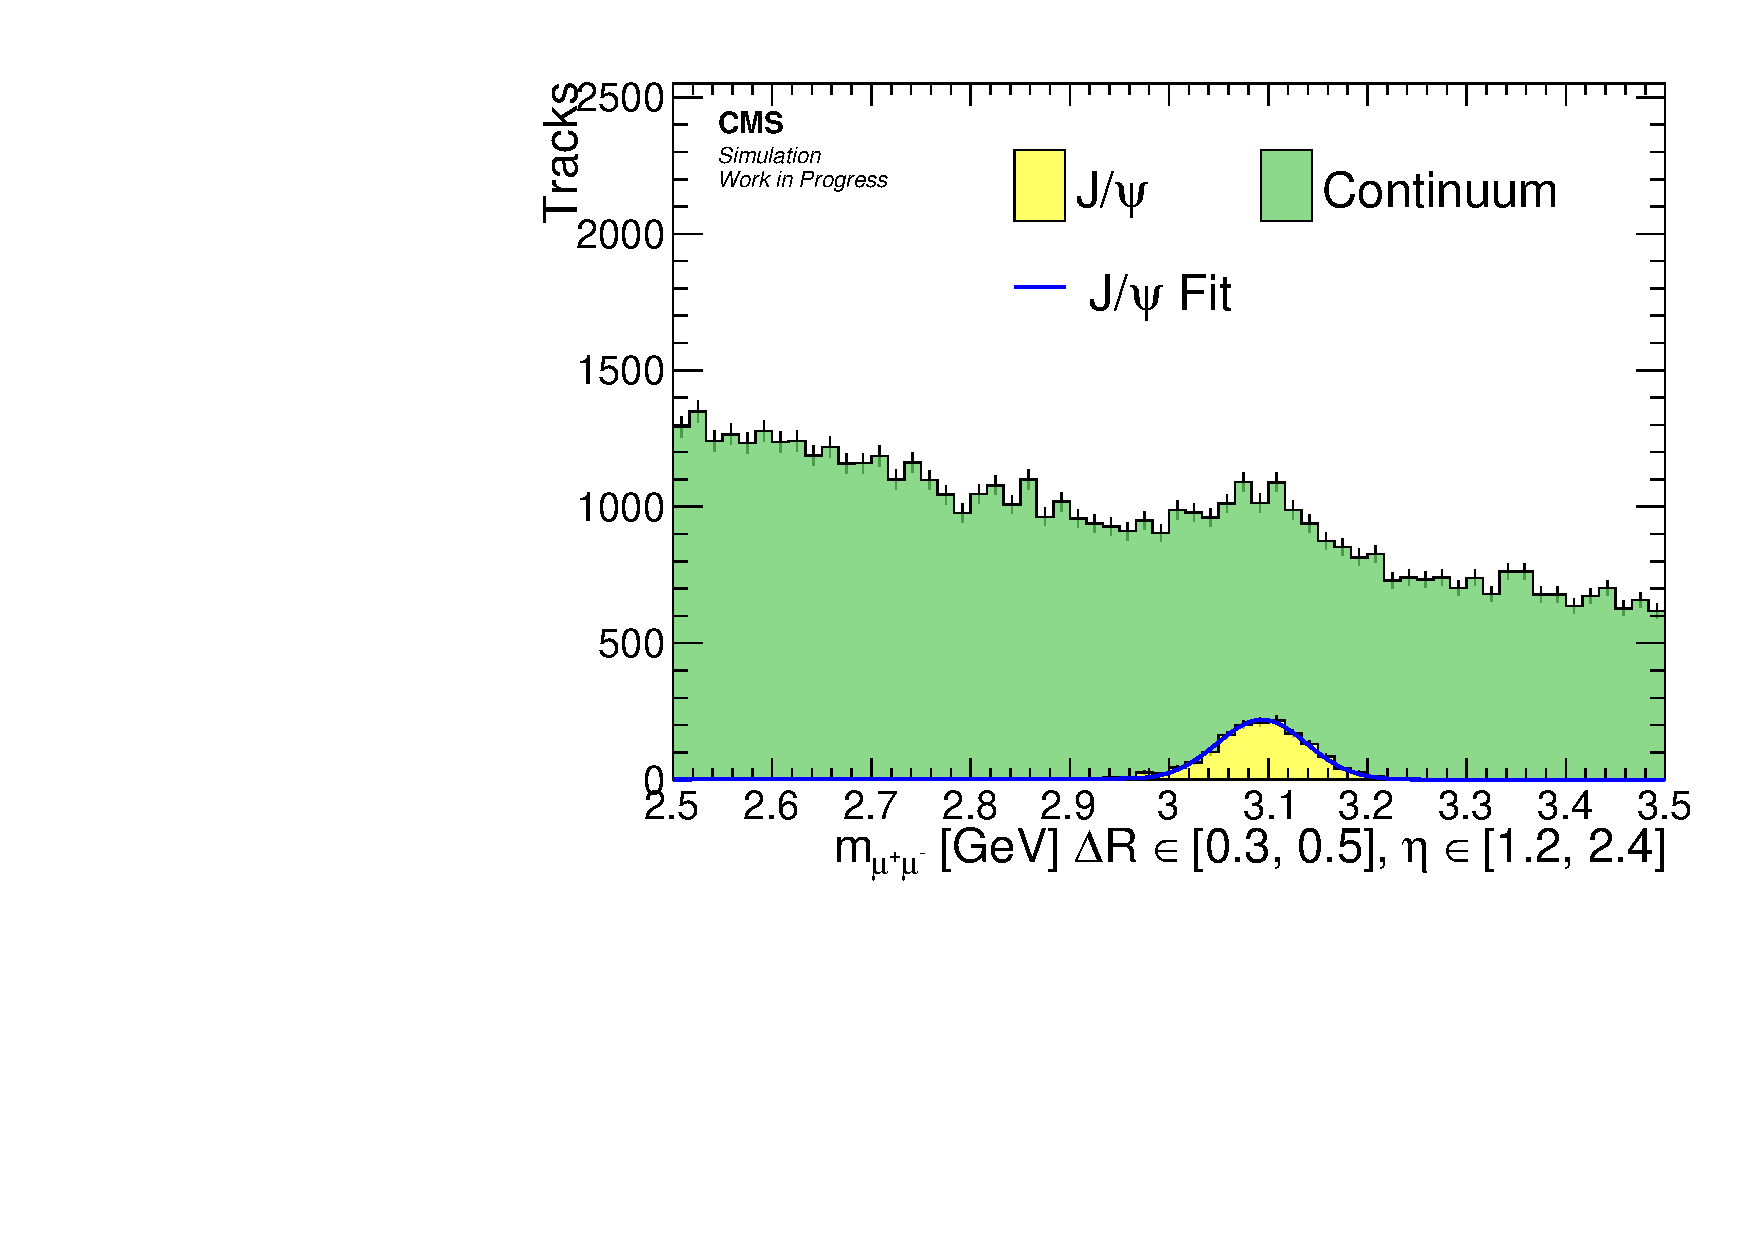
\includegraphics[width=0.32\linewidth]{plots/jpsi_muons_fit_bg_delta_r_single_electron/none_invMass_0.3_0.5_1.2_2.4.pdf} \,
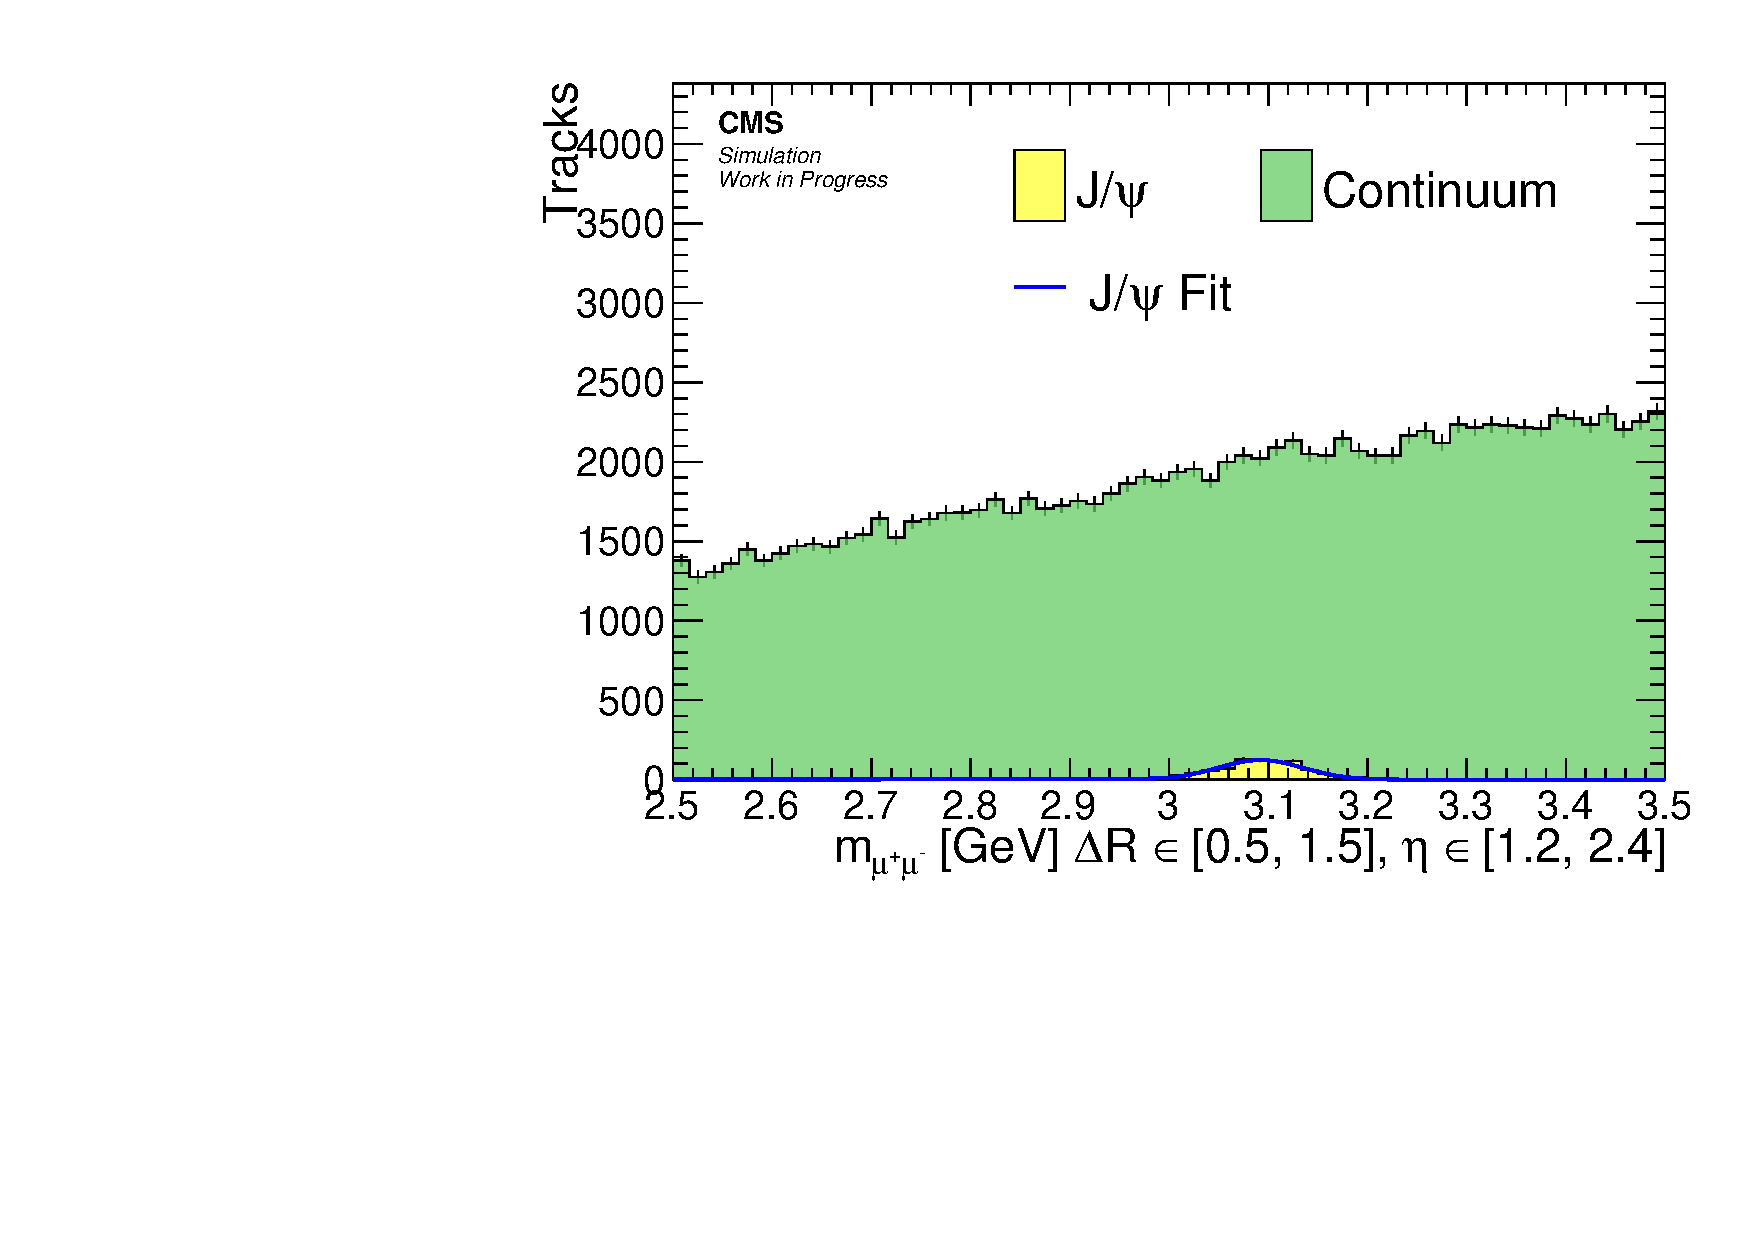
\includegraphics[width=0.32\linewidth]{plots/jpsi_muons_fit_bg_delta_r_single_electron/none_invMass_0.5_1.5_1.2_2.4.pdf} \\
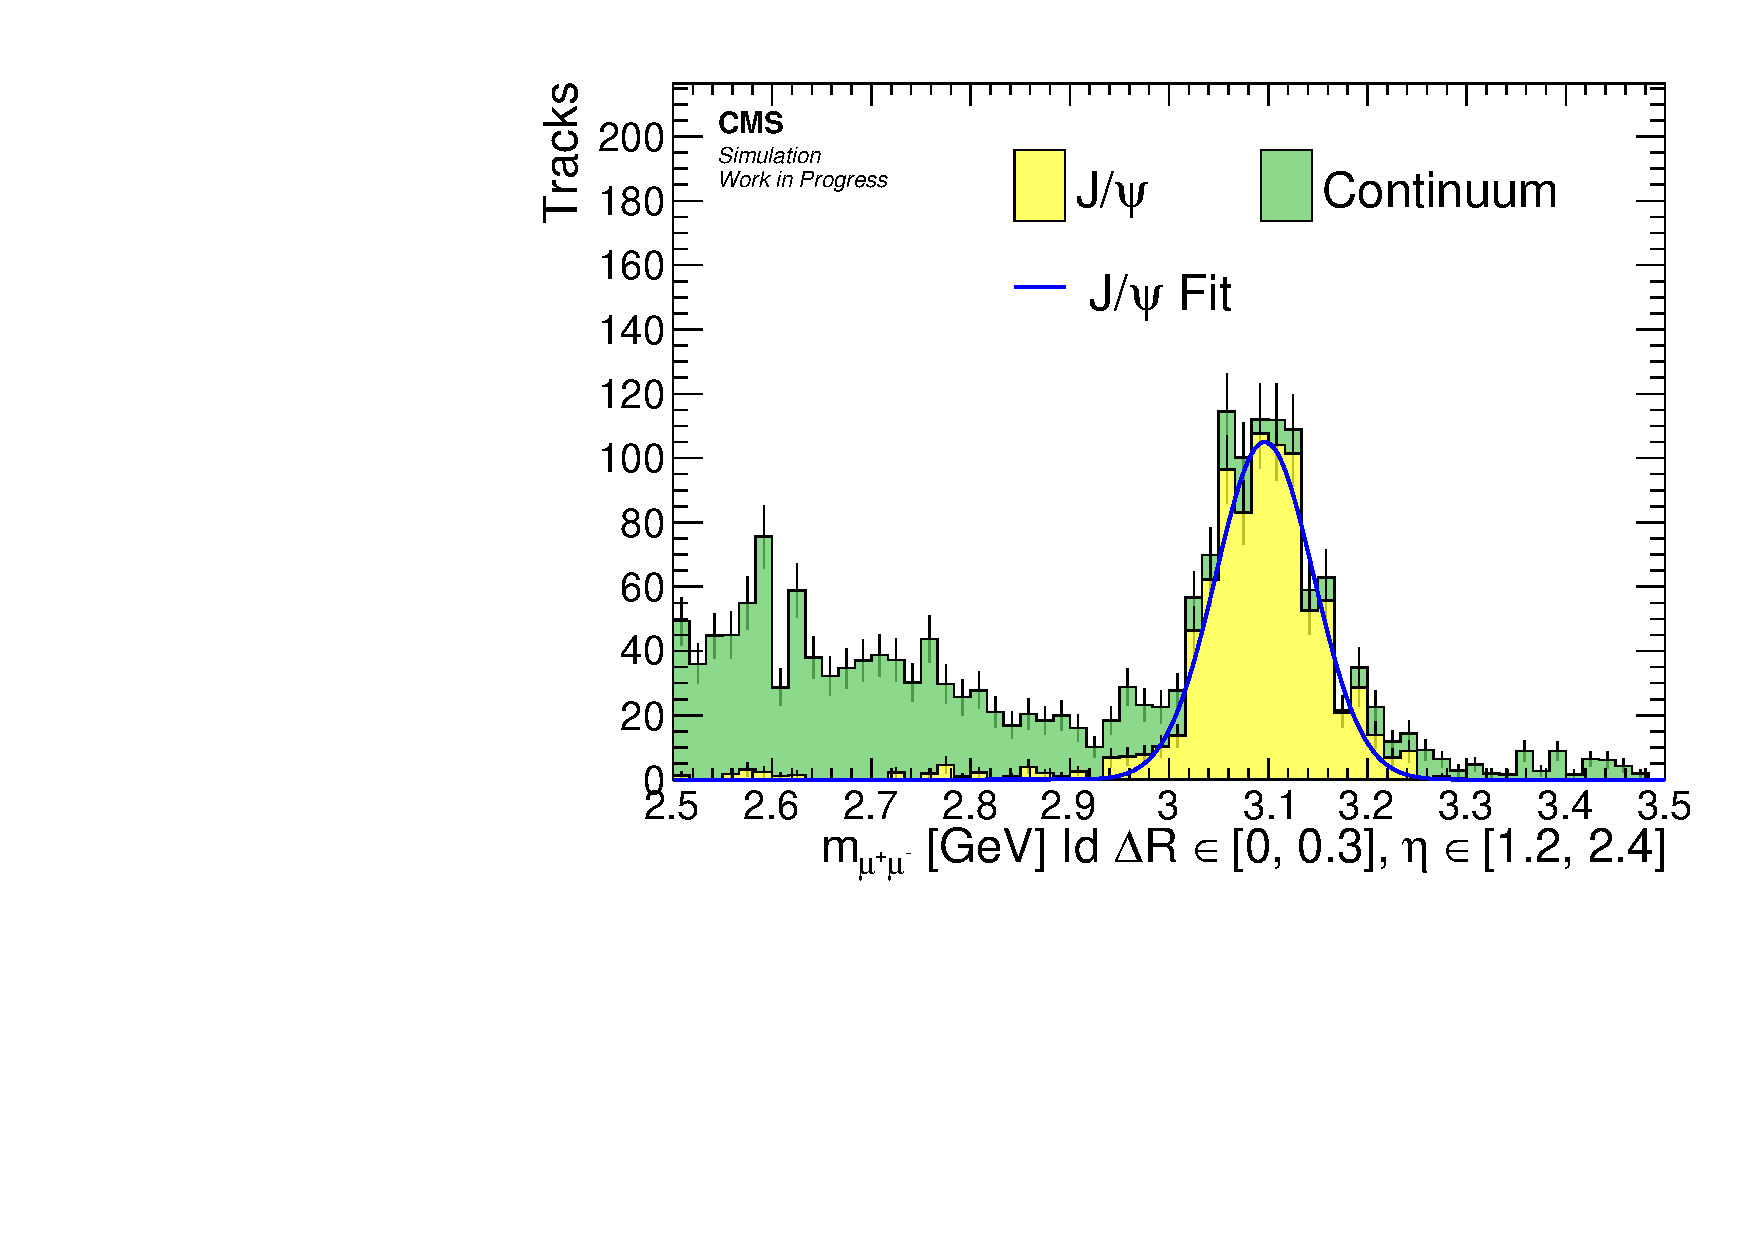
\includegraphics[width=0.32\linewidth]{plots/jpsi_muons_fit_bg_delta_r_single_electron/none_id_invMass_0_0.3_1.2_2.4.pdf} \,
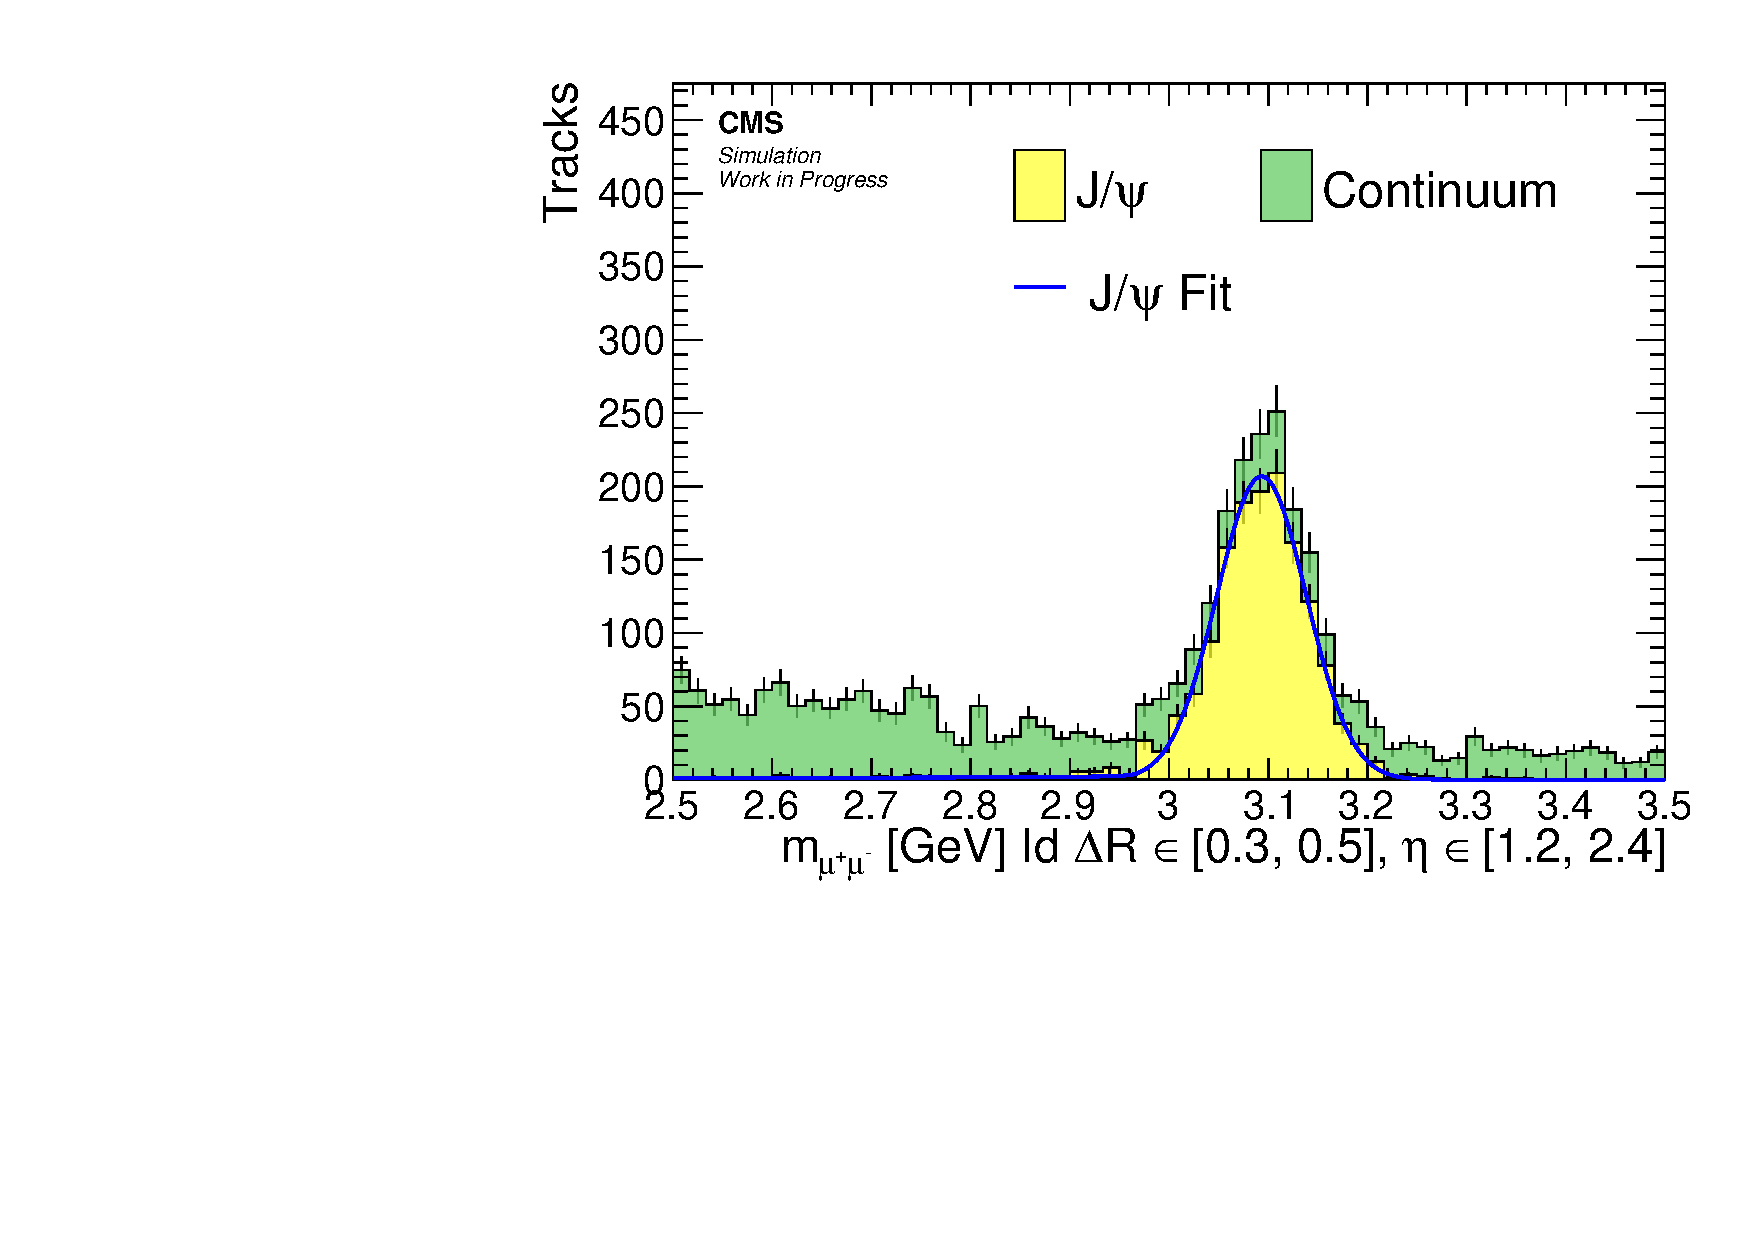
\includegraphics[width=0.32\linewidth]{plots/jpsi_muons_fit_bg_delta_r_single_electron/none_id_invMass_0.3_0.5_1.2_2.4.pdf} \,
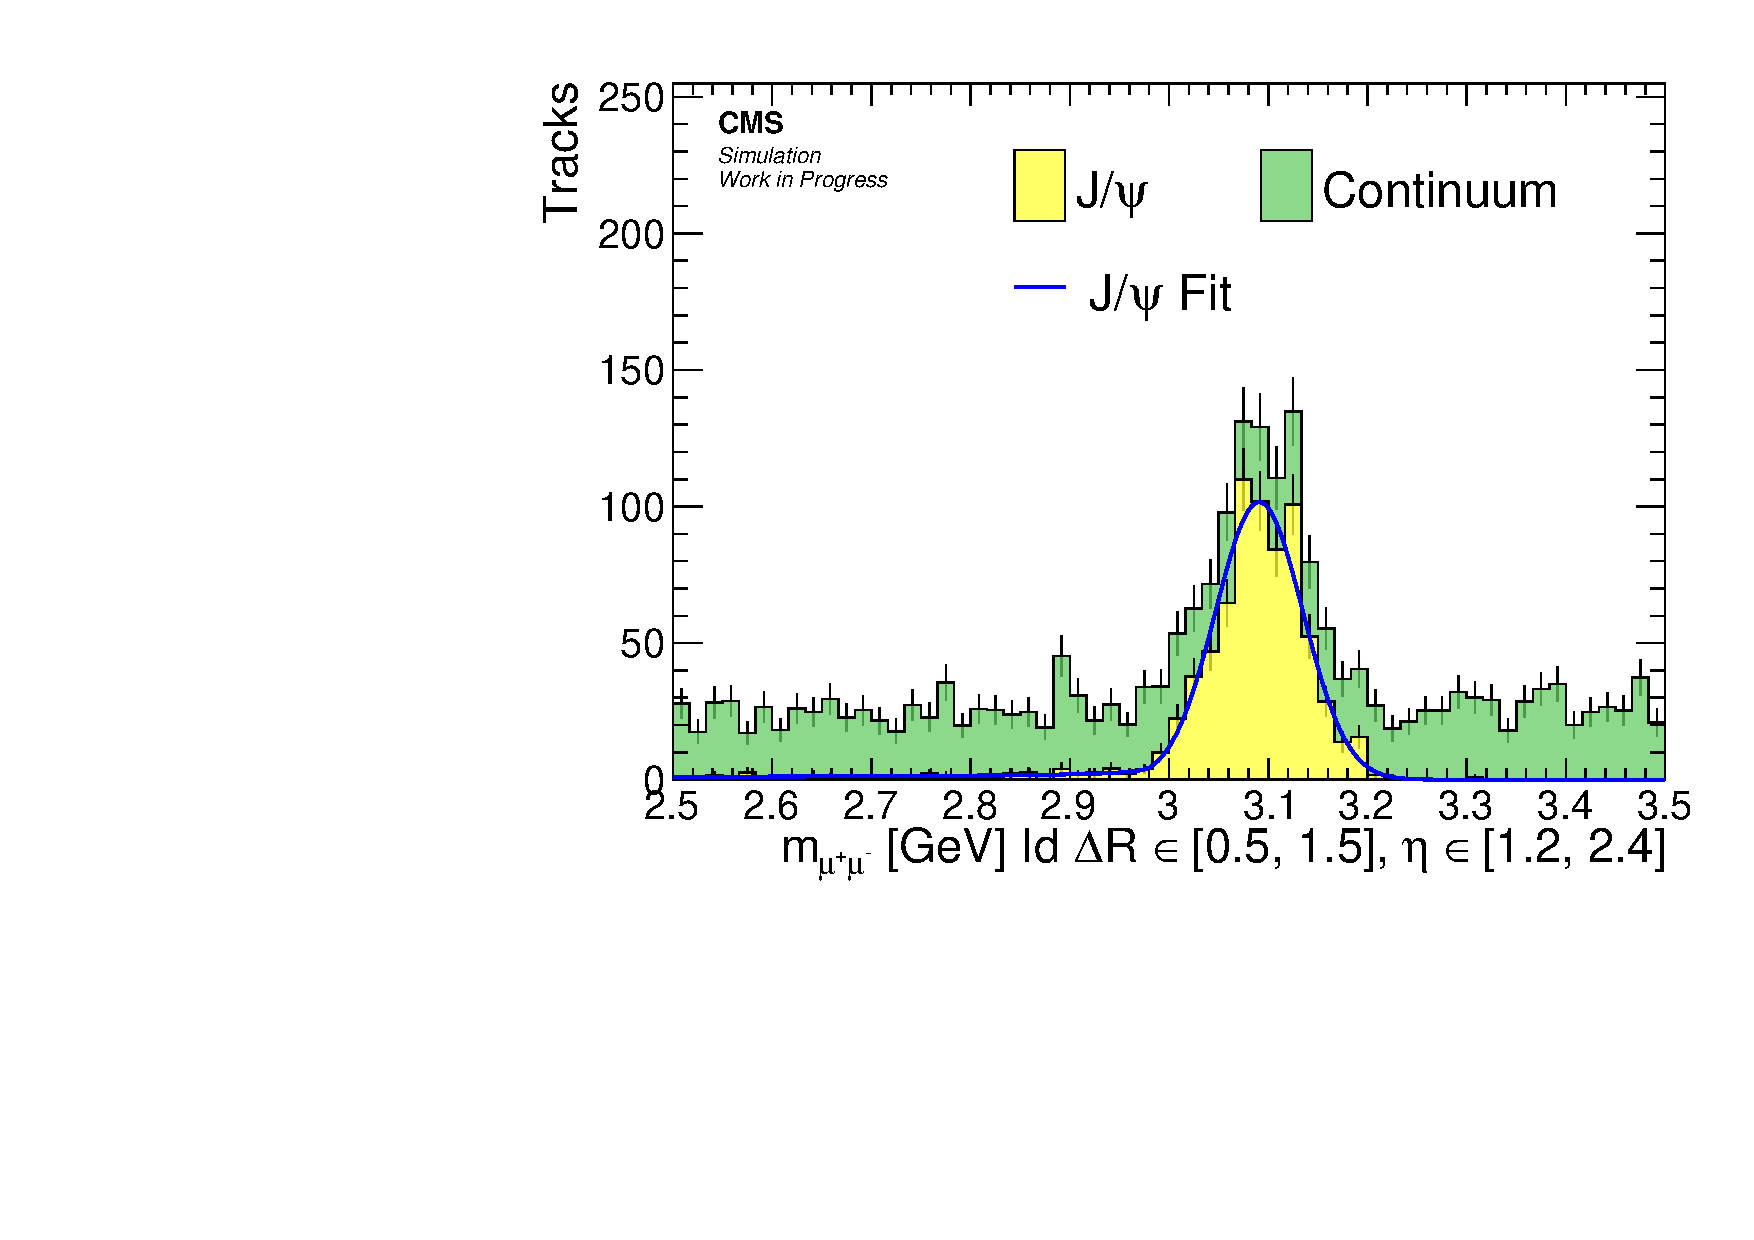
\includegraphics[width=0.32\linewidth]{plots/jpsi_muons_fit_bg_delta_r_single_electron/none_id_invMass_0.5_1.5_1.2_2.4.pdf}  \\
\caption[Endcaps BG]{Endcaps Muons BG}
\label{fig:tb-endcaps-simulation}
\end{figure}

\begin{figure}[]
\centering
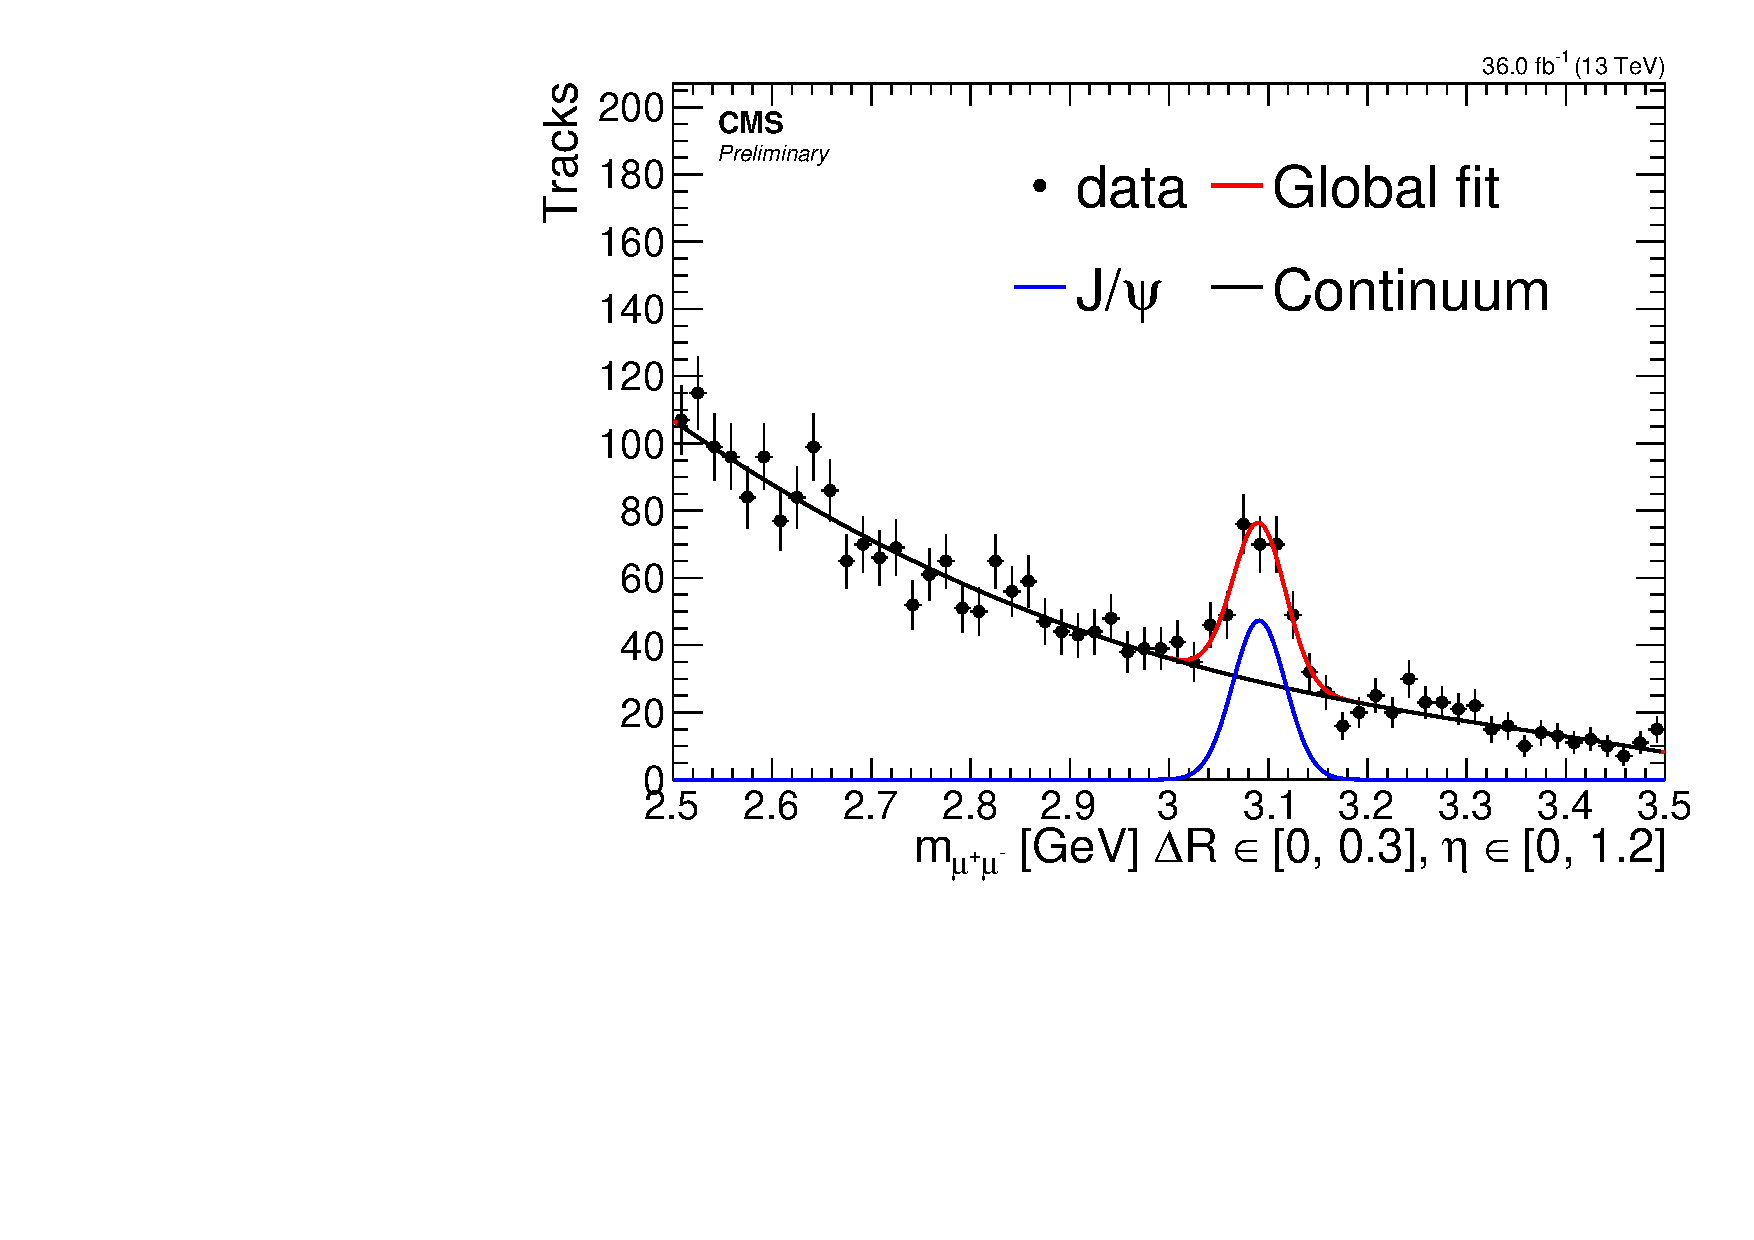
\includegraphics[width=0.32\linewidth]{plots/jpsi_muons_fit_data_delta_r_single_electron/none_invMass_0_0.3_0_1.2.pdf} \,
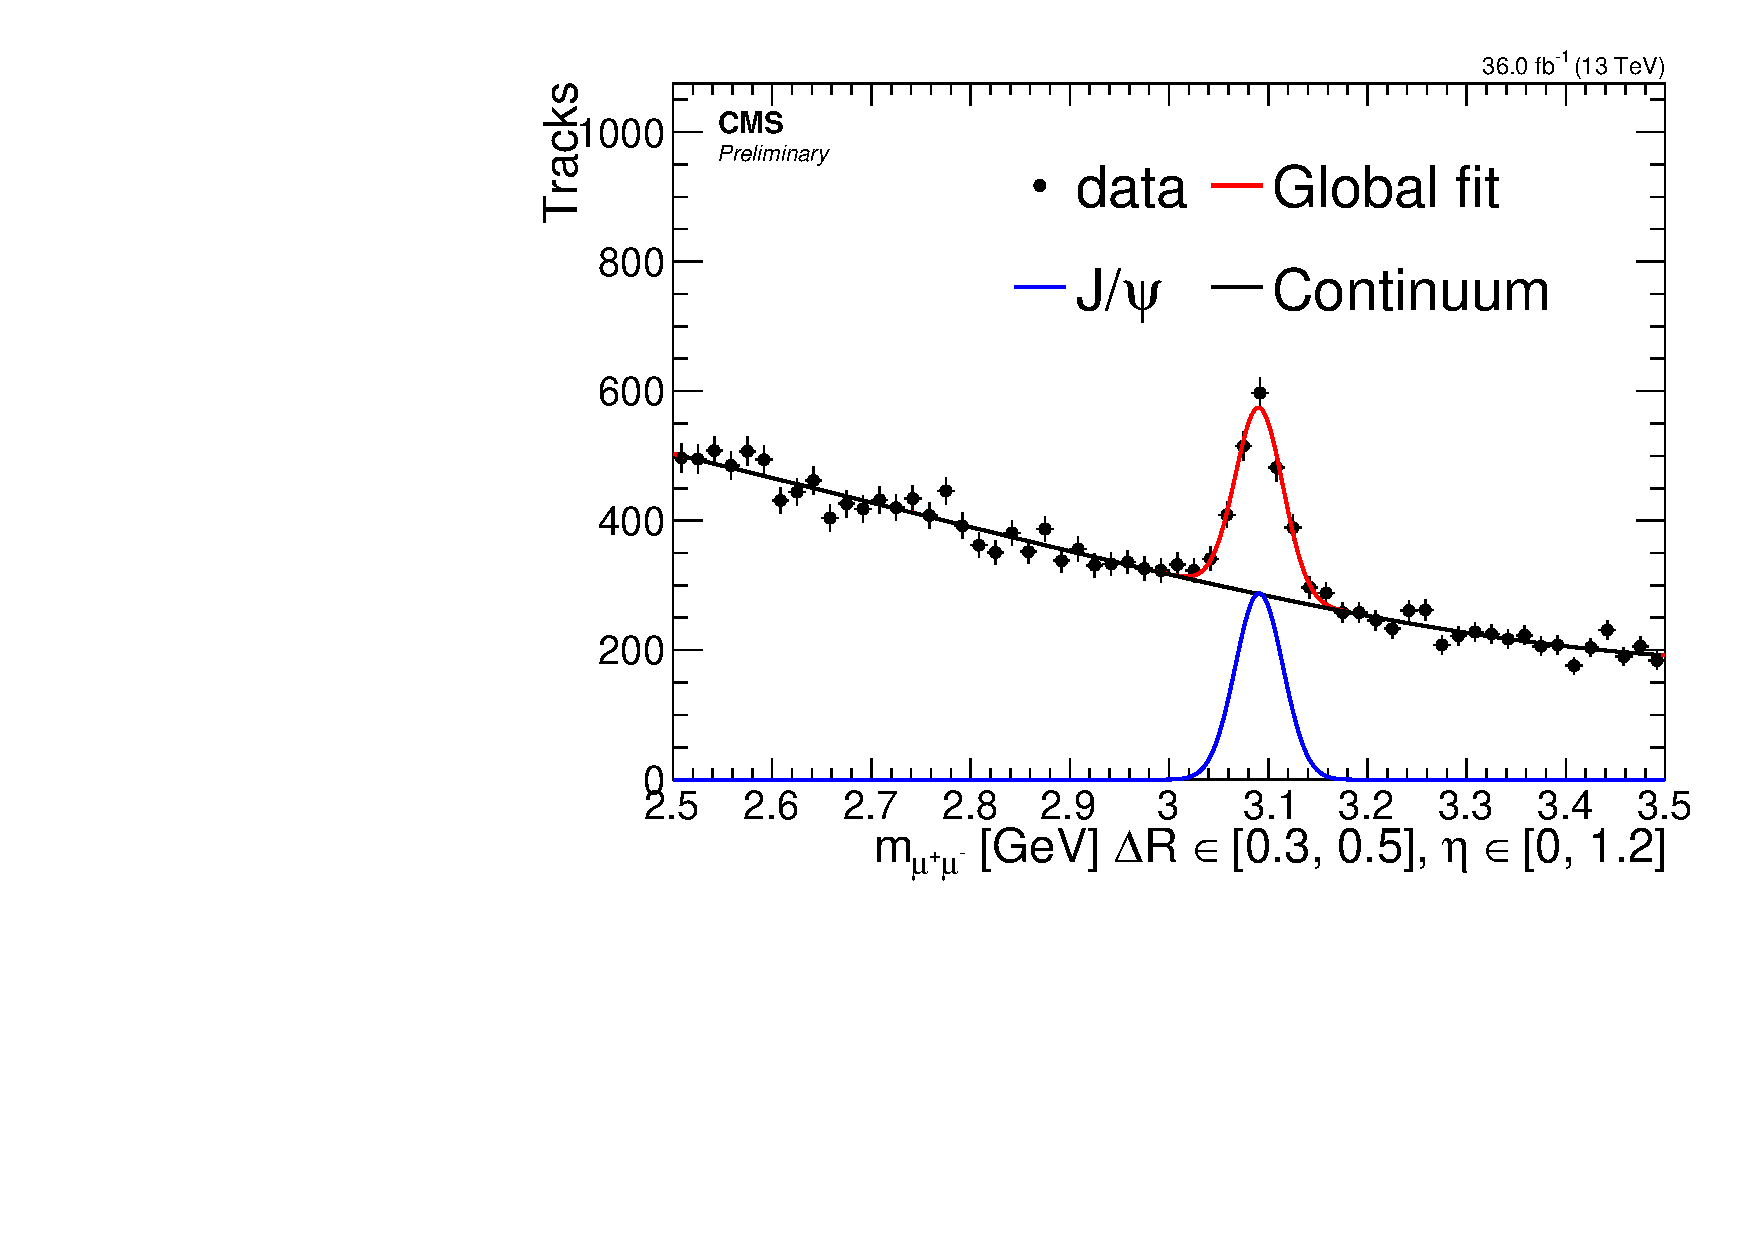
\includegraphics[width=0.32\linewidth]{plots/jpsi_muons_fit_data_delta_r_single_electron/none_invMass_0.3_0.5_0_1.2.pdf}  \,
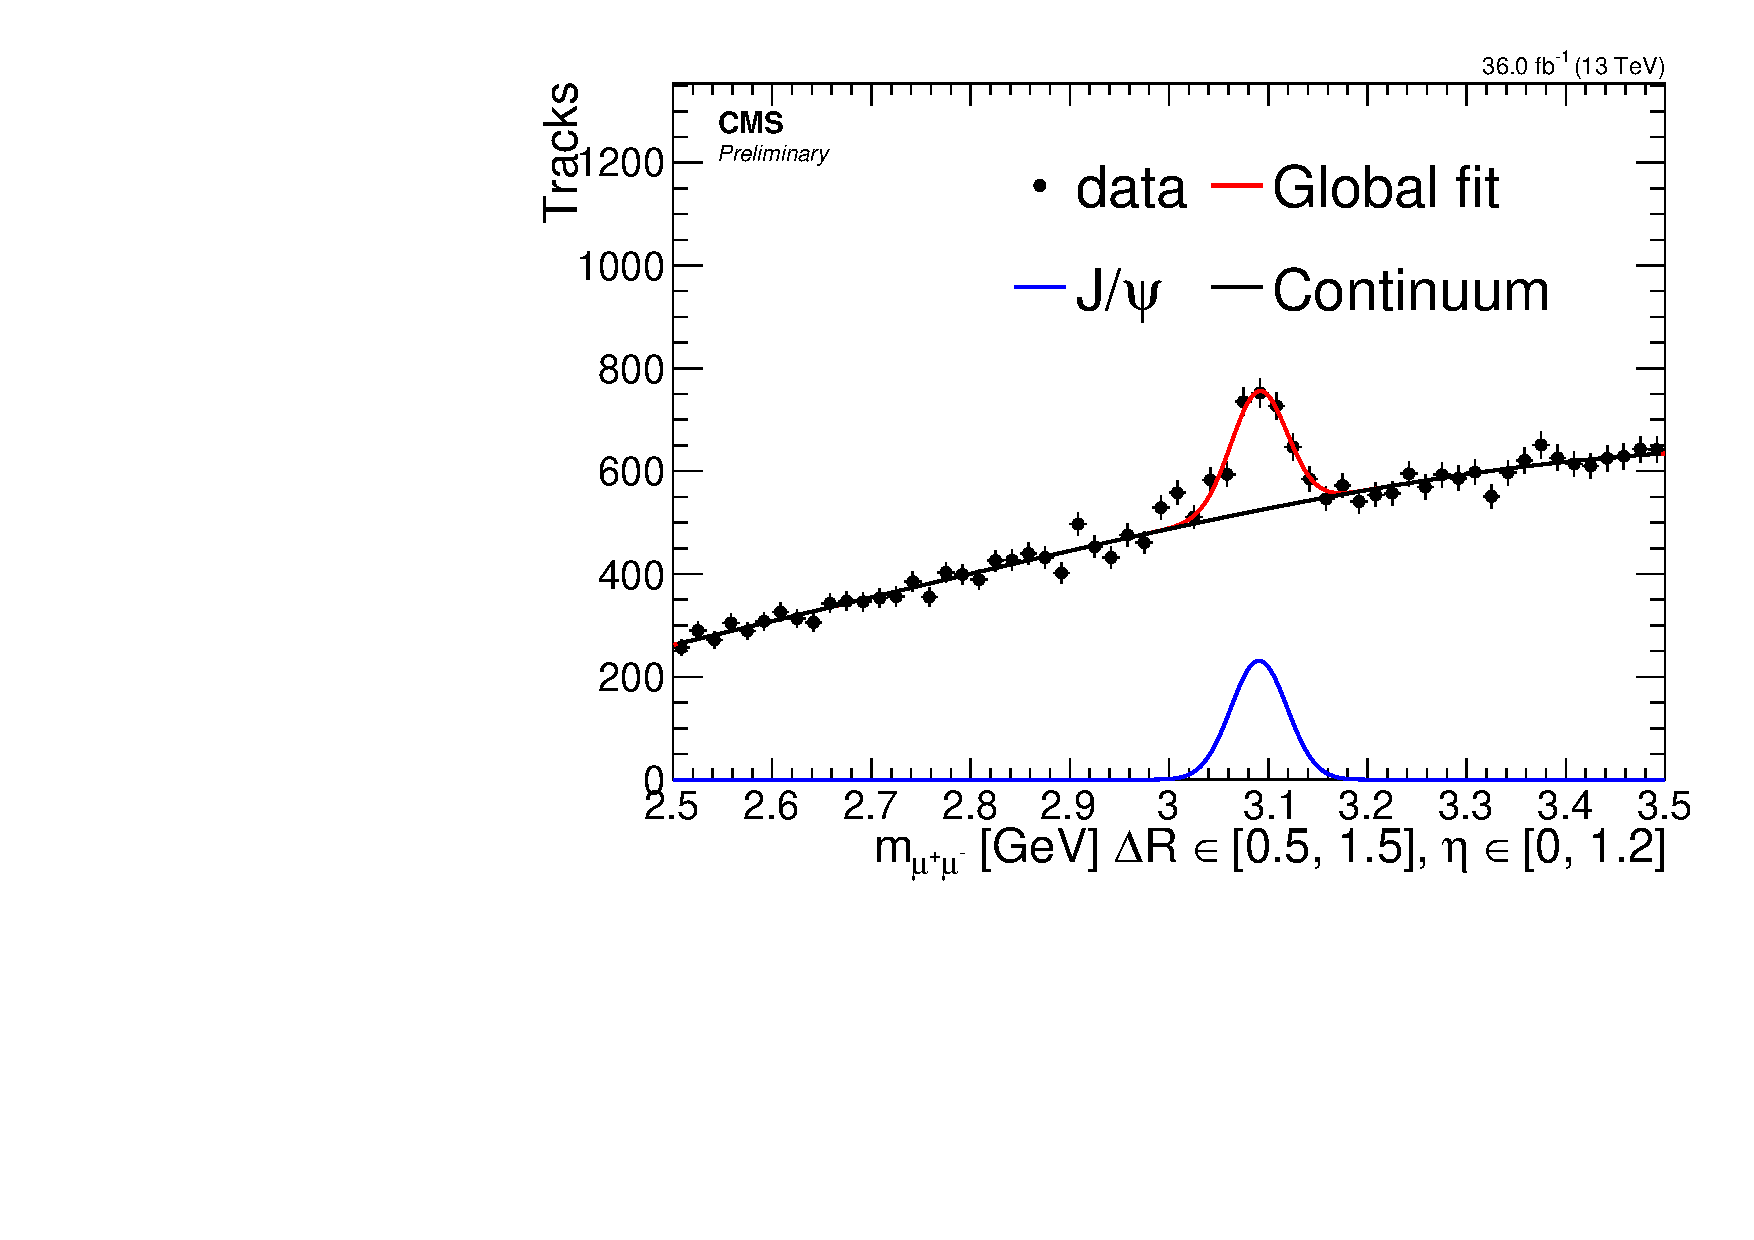
\includegraphics[width=0.32\linewidth]{plots/jpsi_muons_fit_data_delta_r_single_electron/none_invMass_0.5_1.5_0_1.2.pdf} \\
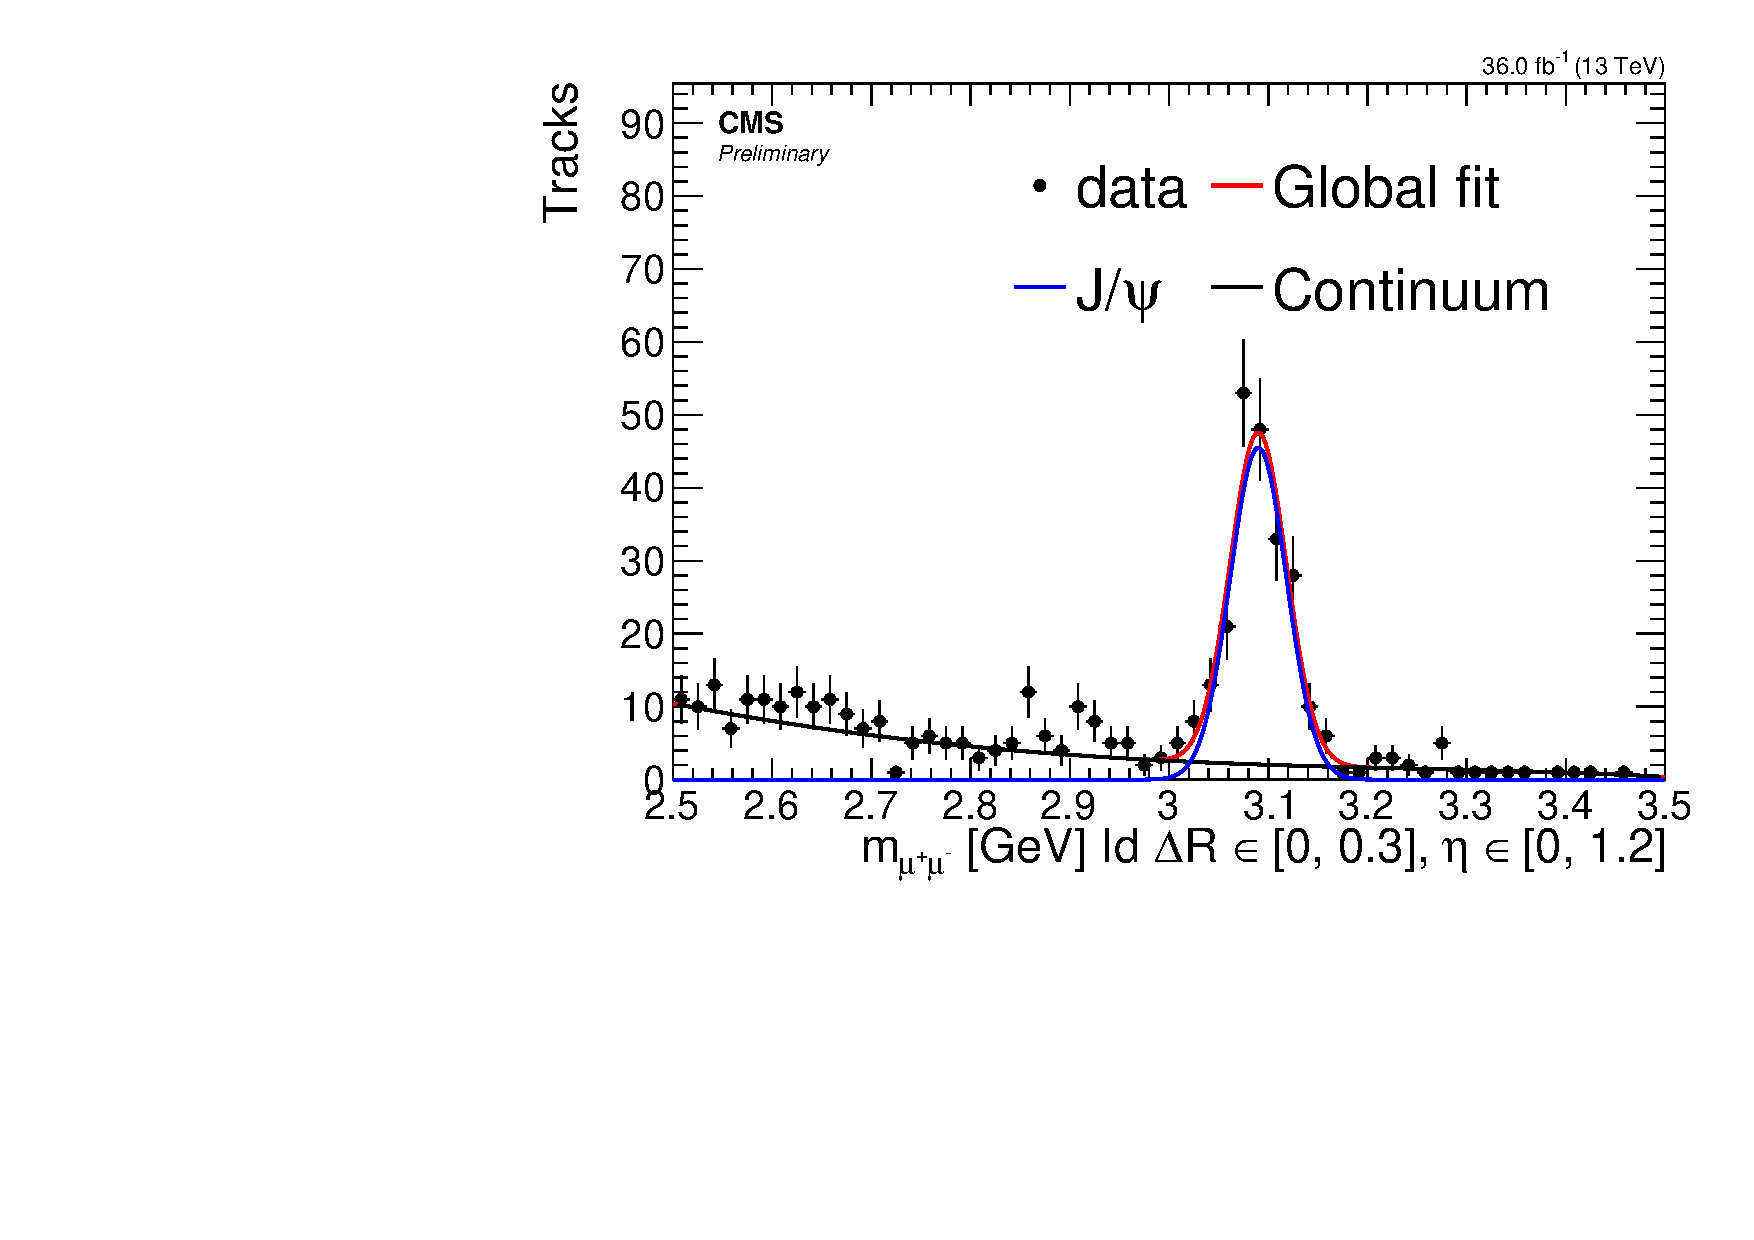
\includegraphics[width=0.32\linewidth]{plots/jpsi_muons_fit_data_delta_r_single_electron/none_id_invMass_0_0.3_0_1.2.pdf} \,
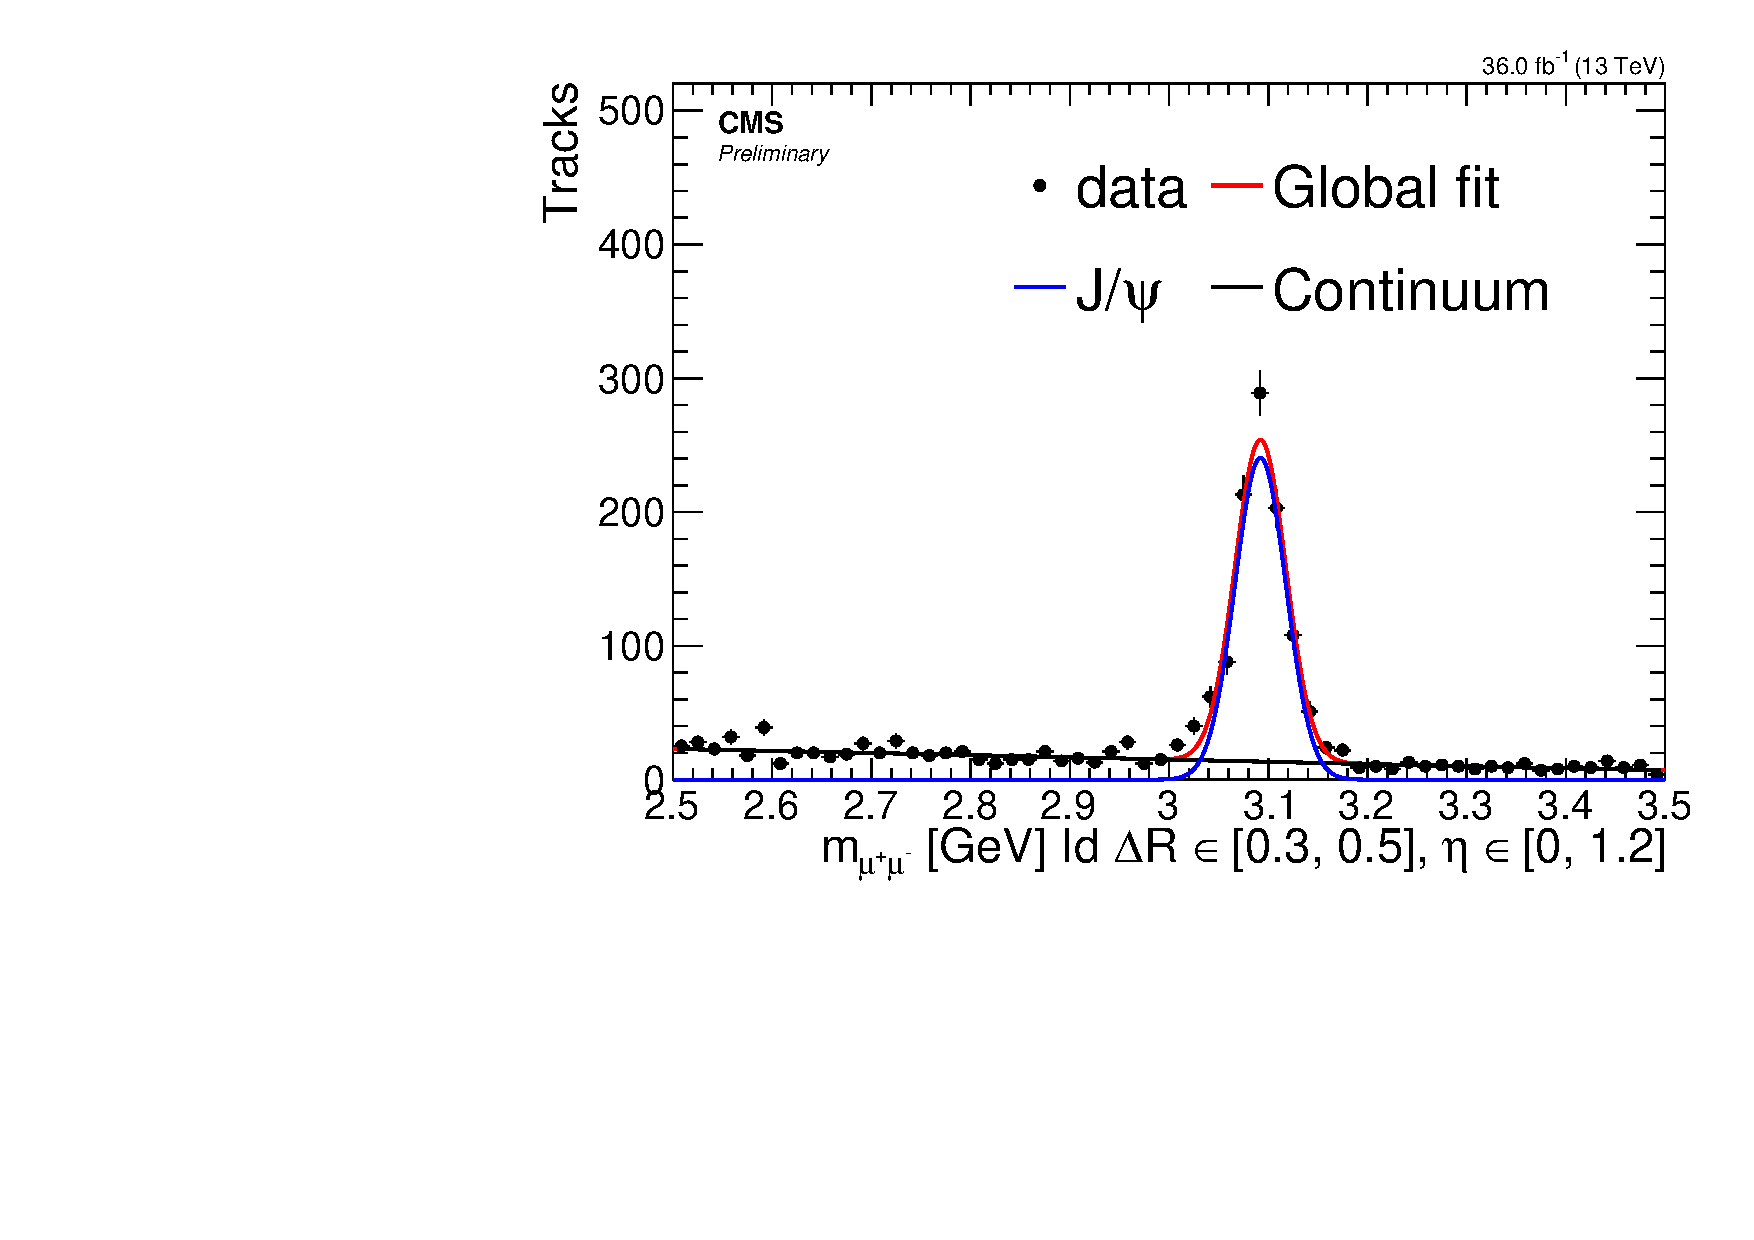
\includegraphics[width=0.32\linewidth]{plots/jpsi_muons_fit_data_delta_r_single_electron/none_id_invMass_0.3_0.5_0_1.2.pdf}  \,
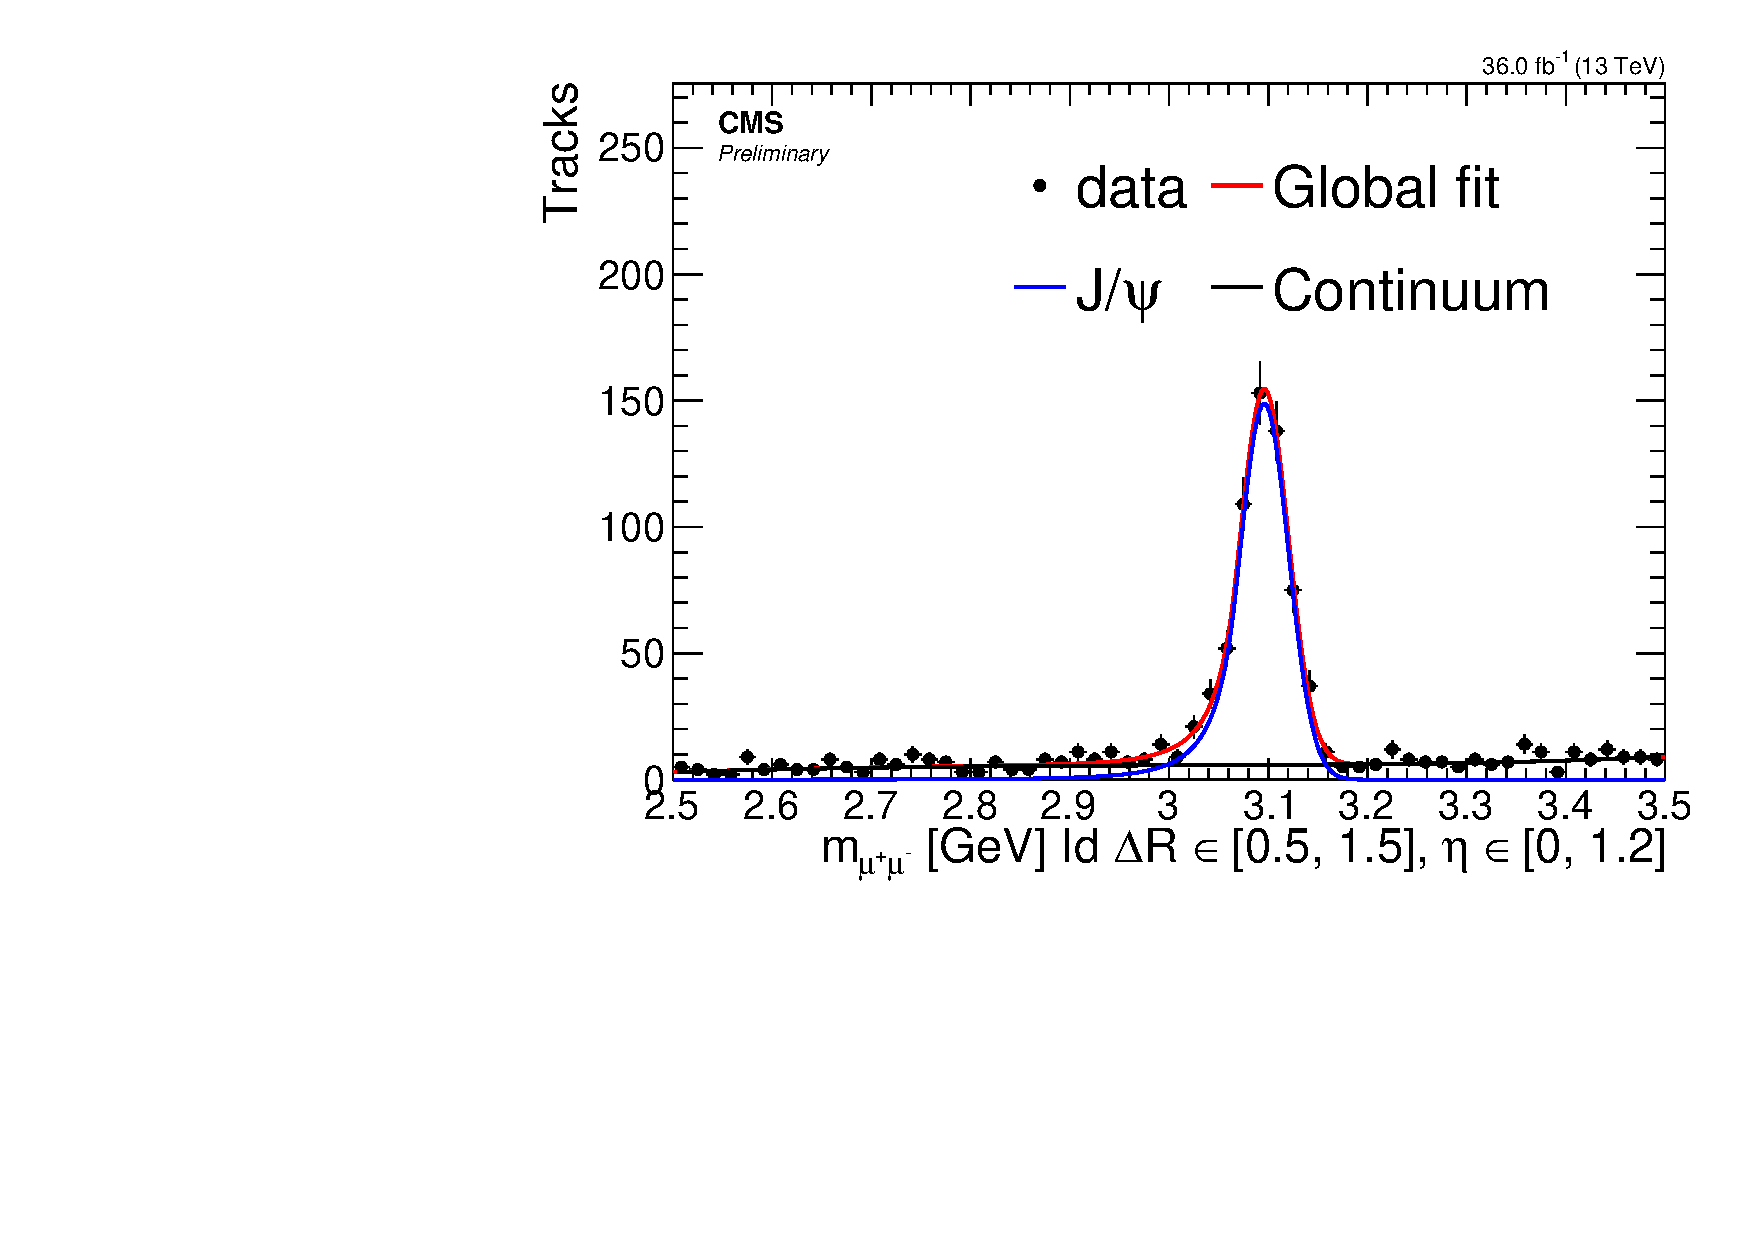
\includegraphics[width=0.32\linewidth]{plots/jpsi_muons_fit_data_delta_r_single_electron/none_id_invMass_0.5_1.5_0_1.2.pdf} \\
\caption[Barrel Data]{Barrel Muons Data}
\label{fig:tb-barrel-data}
\end{figure}

\begin{figure}[]
\centering
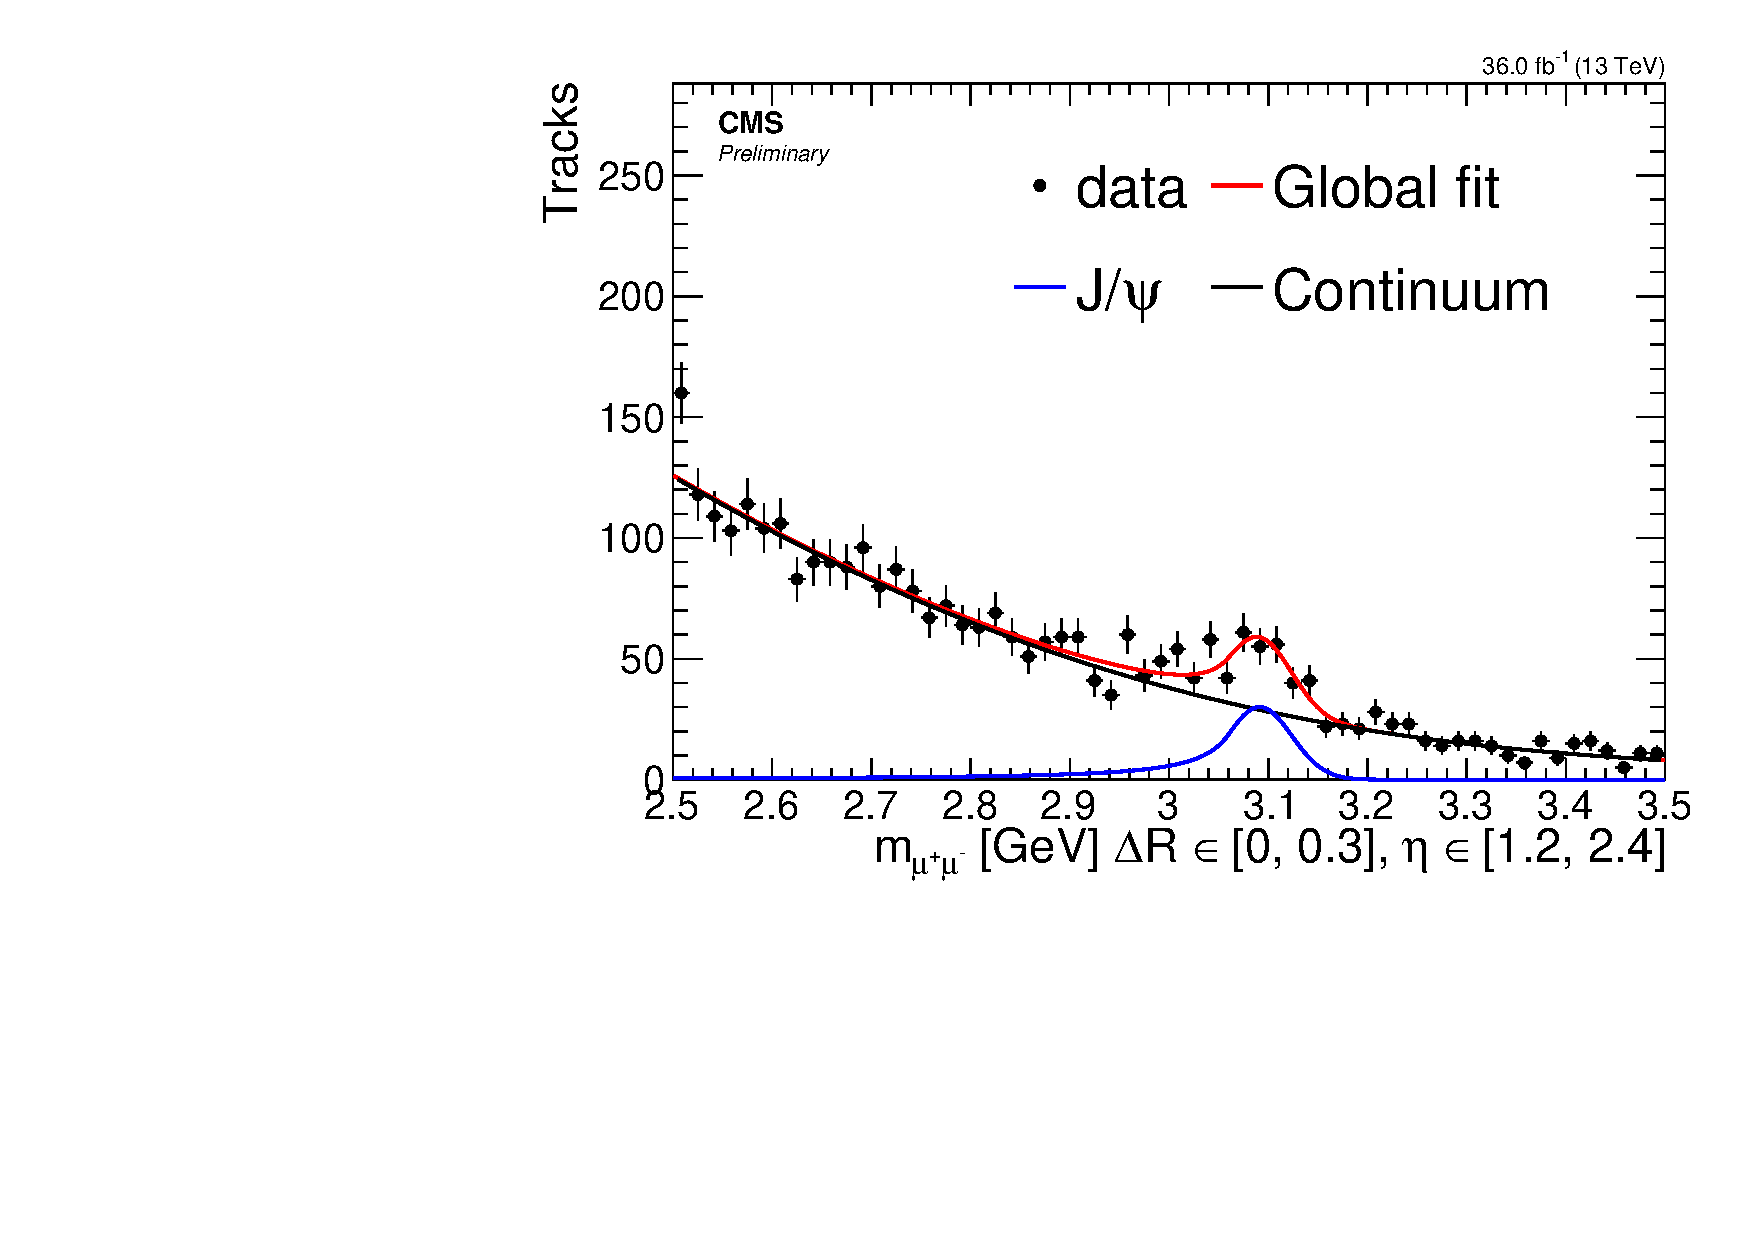
\includegraphics[width=0.32\linewidth]{plots/jpsi_muons_fit_data_delta_r_single_electron/none_invMass_0_0.3_1.2_2.4.pdf} \,
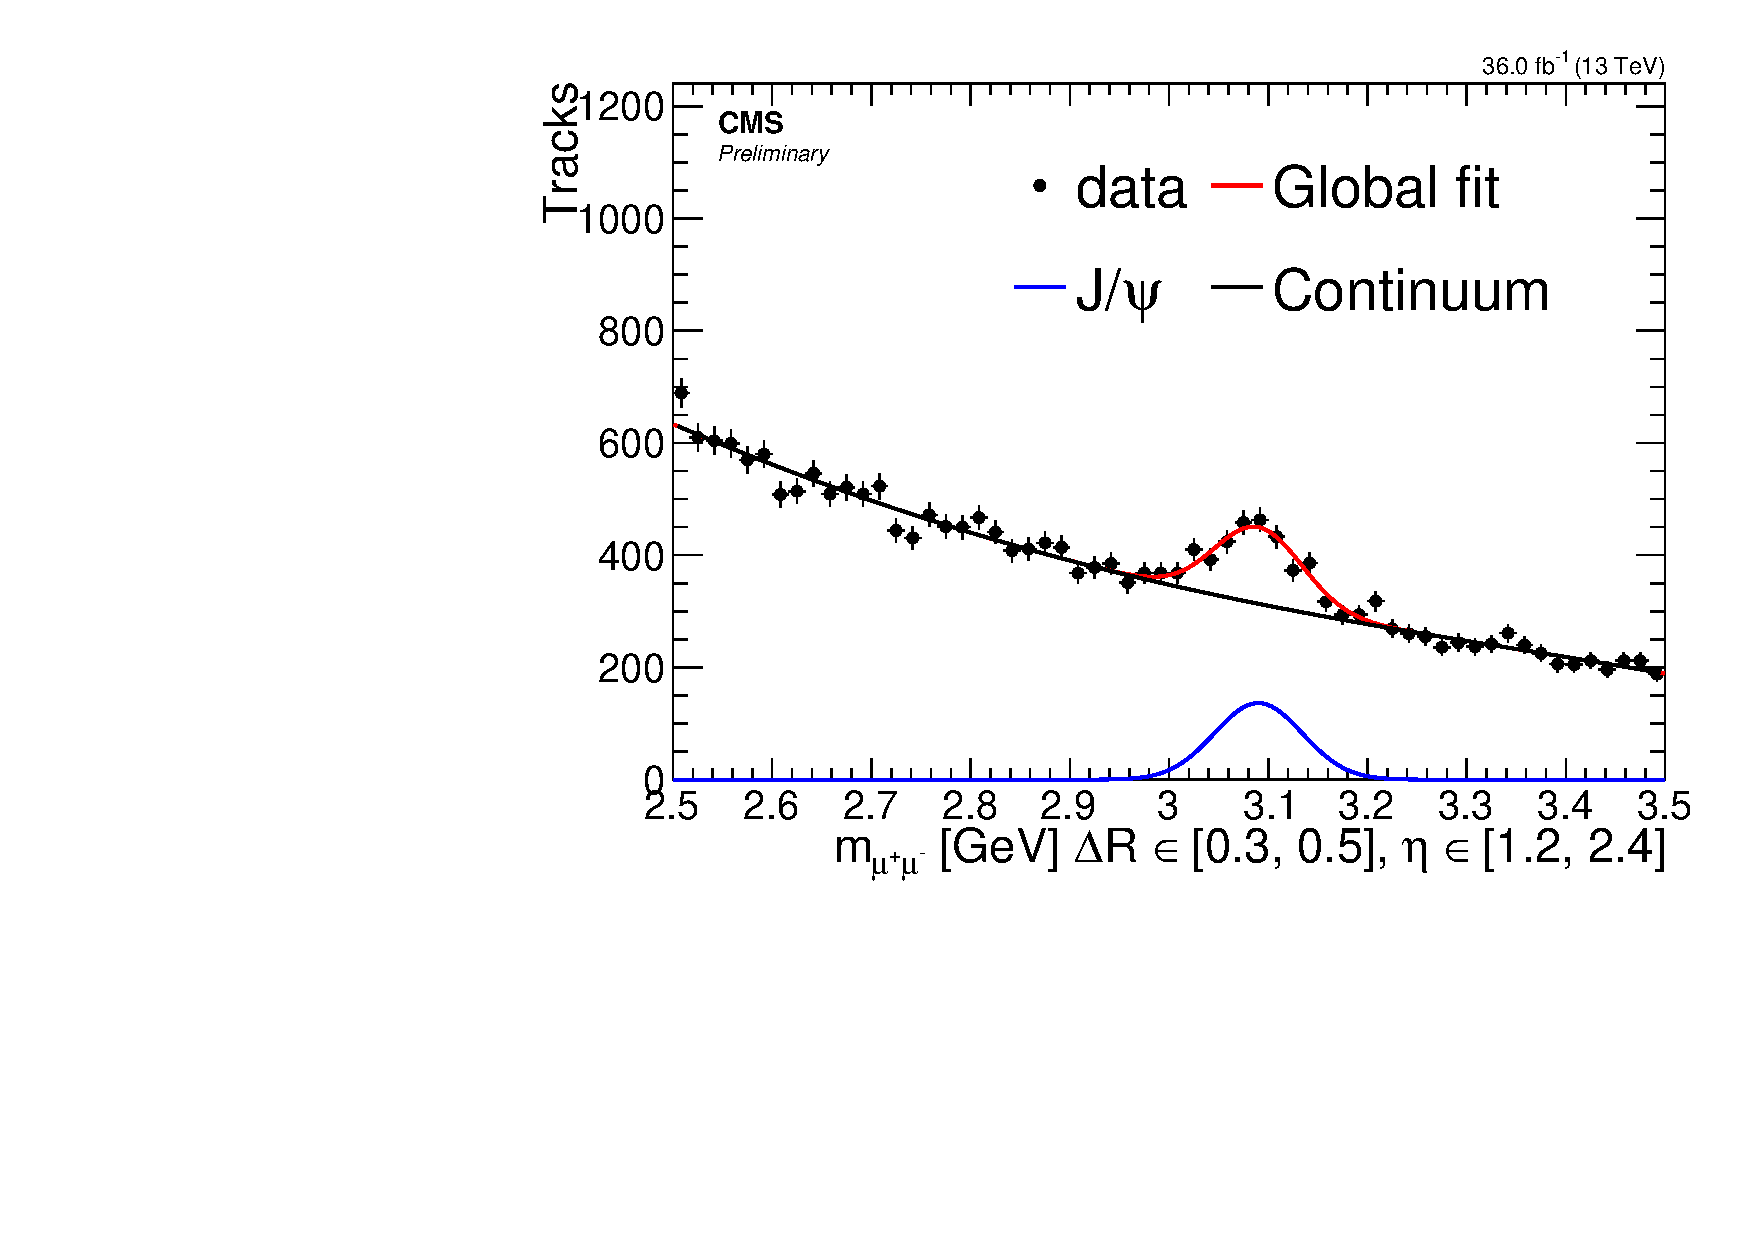
\includegraphics[width=0.32\linewidth]{plots/jpsi_muons_fit_data_delta_r_single_electron/none_invMass_0.3_0.5_1.2_2.4.pdf} \,
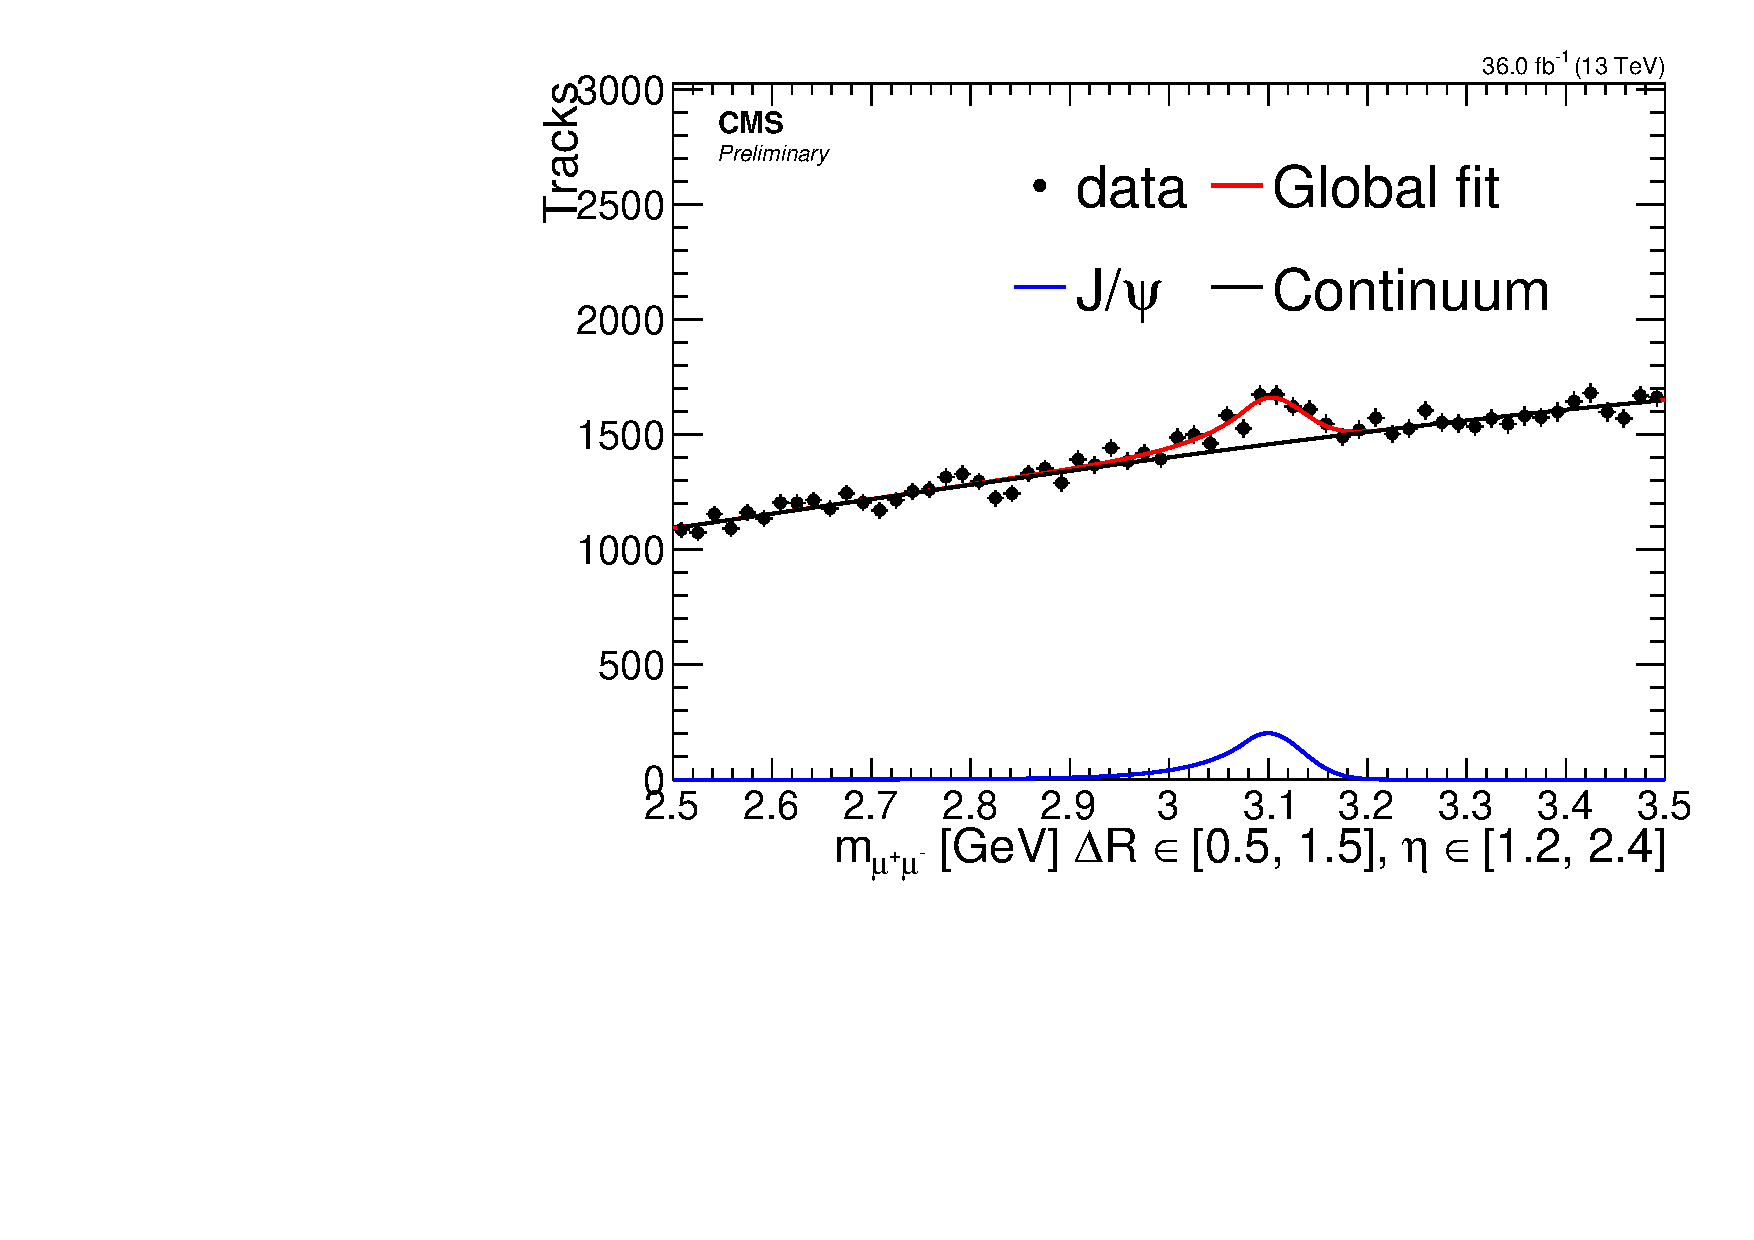
\includegraphics[width=0.32\linewidth]{plots/jpsi_muons_fit_data_delta_r_single_electron/none_invMass_0.5_1.5_1.2_2.4.pdf} \\
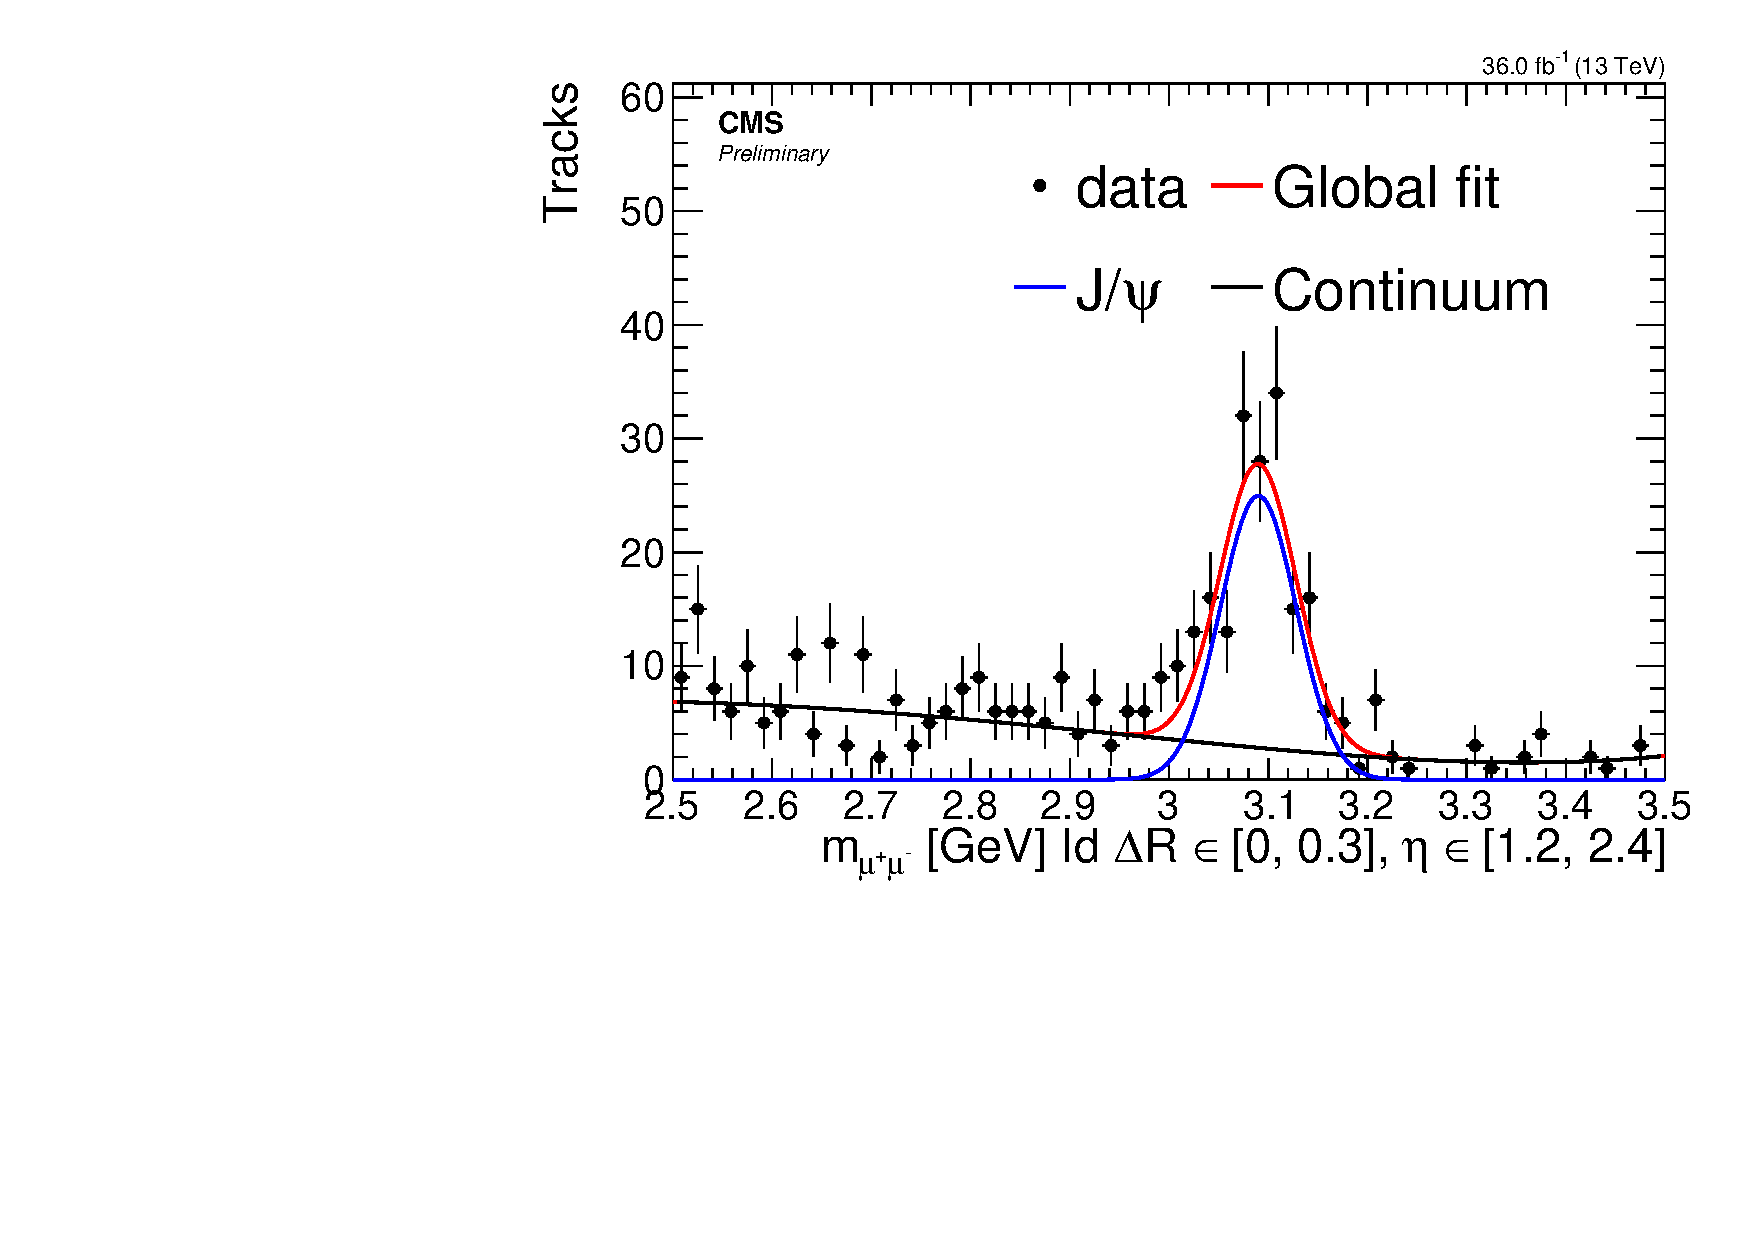
\includegraphics[width=0.32\linewidth]{plots/jpsi_muons_fit_data_delta_r_single_electron/none_id_invMass_0_0.3_1.2_2.4.pdf} \,
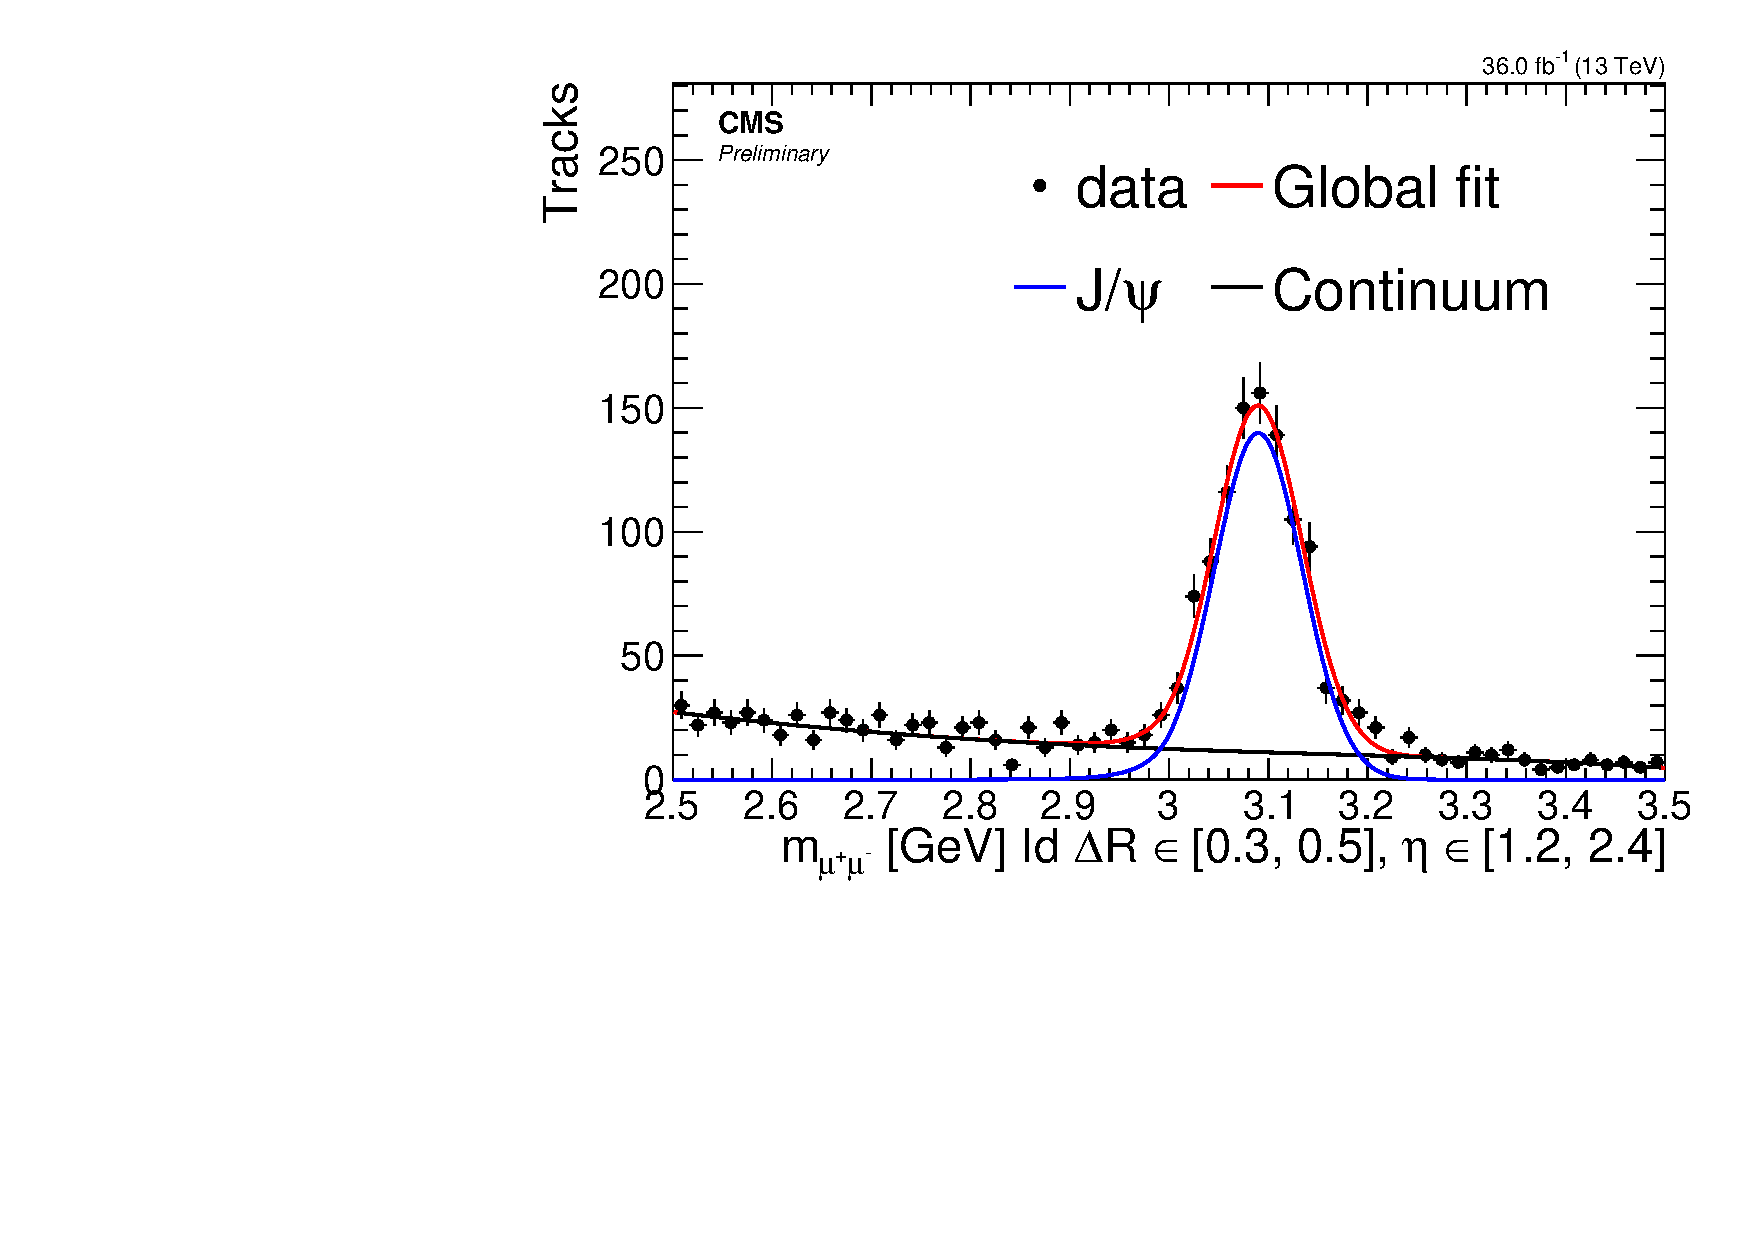
\includegraphics[width=0.32\linewidth]{plots/jpsi_muons_fit_data_delta_r_single_electron/none_id_invMass_0.3_0.5_1.2_2.4.pdf} \,
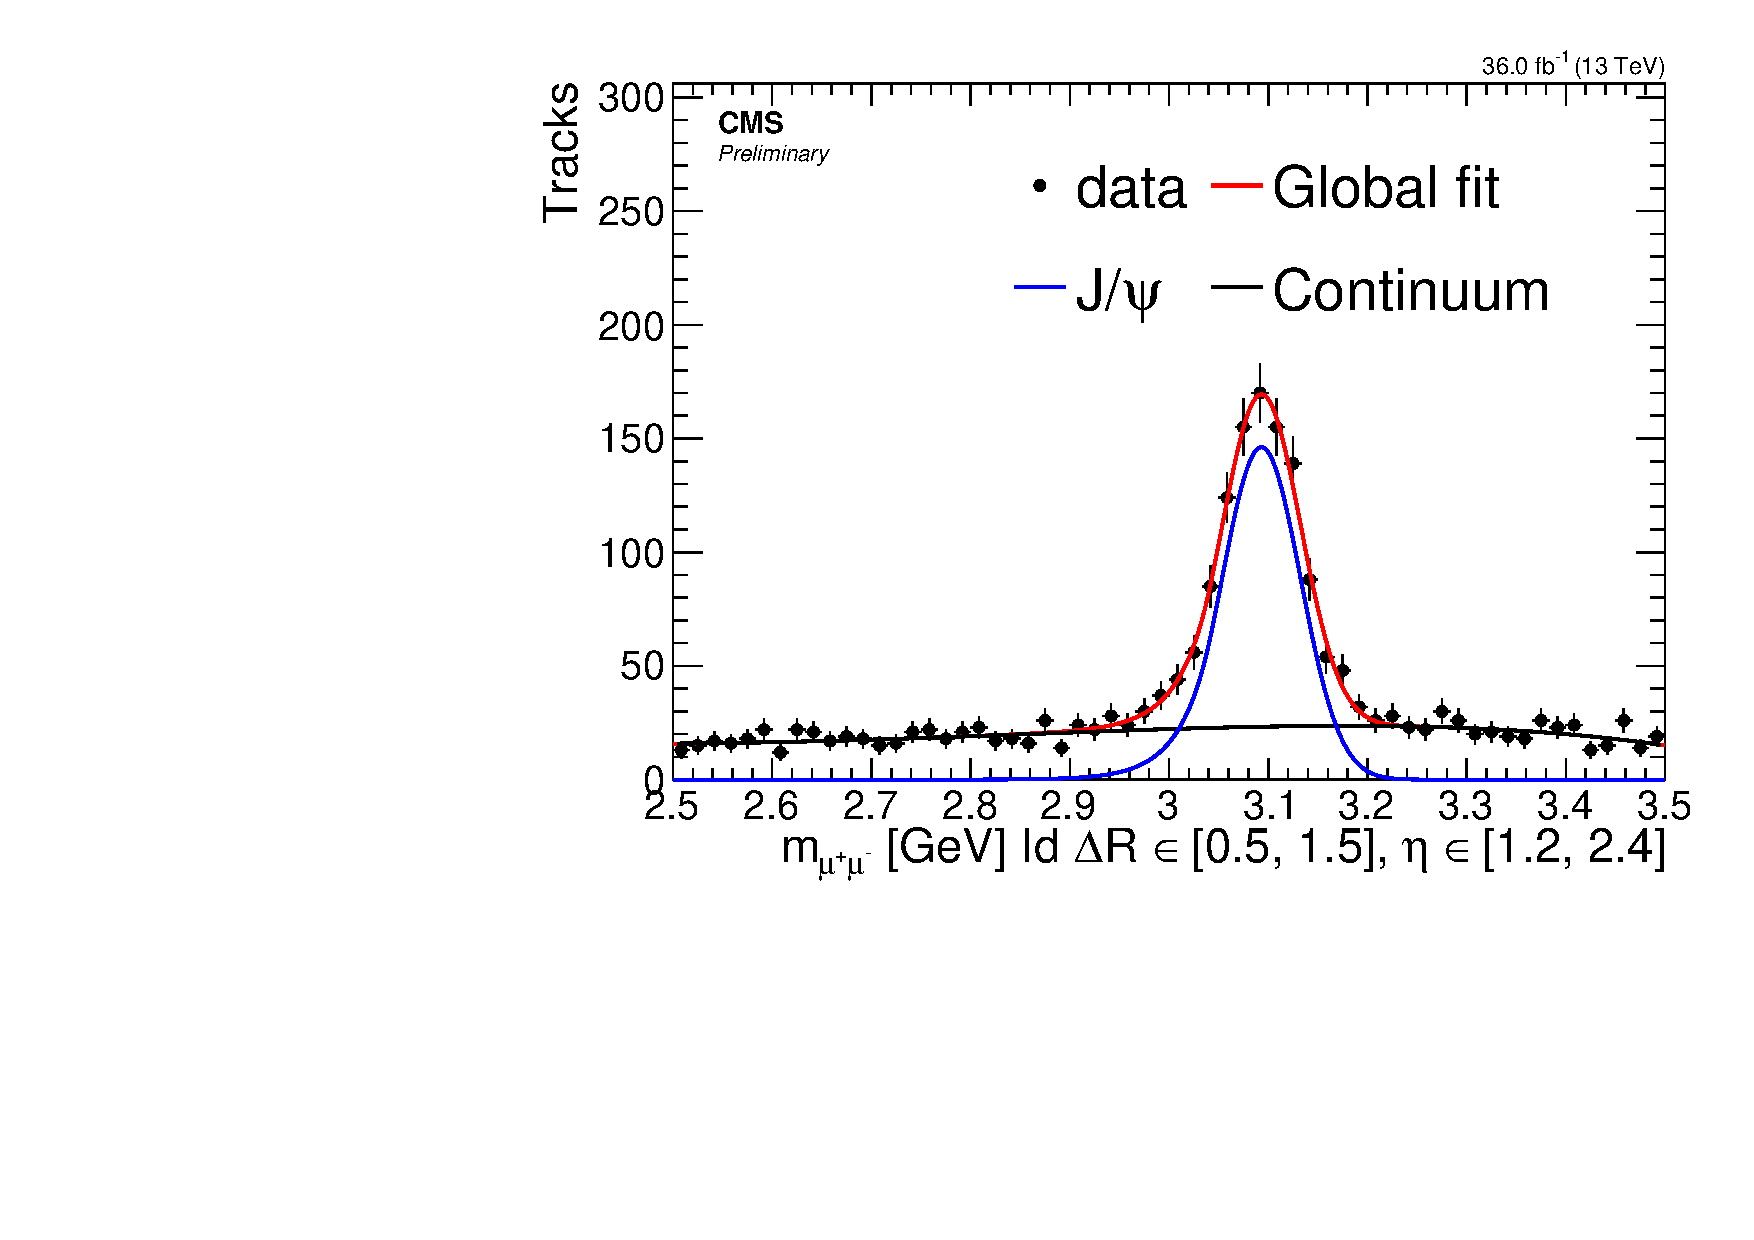
\includegraphics[width=0.32\linewidth]{plots/jpsi_muons_fit_data_delta_r_single_electron/none_id_invMass_0.5_1.5_1.2_2.4.pdf}  \\
\caption[Endcaps Data]{Endcaps Muons Data}
\label{fig:tb-endcaps-data}
\end{figure}

\subsection{Tracks and multivariate selection }
\subsection{Isolation}
\label{sec:isolation}
